%\chapter{Optical Response of Metallic Zigzag Bigratings}
\section{Background}
This chapter introduces a novel type of diffraction grating, the zigzag grating. A detailed experimental and theoretical study of the SPPs excited on such a grating is explored, with interesting results pertaining to the polarisation requirements of the coupled light, the plasmonic band-gap character of interacting SPP modes, and the highly anisotropic propagation of SPP on such a grating. 

In 2005, Kleemann et al. \cite{Kleemann2005} presented a new method for designing diffractive optical elements with efficiencies and properties comparable to traditional surface relief gratings. These gratings use sub-wavelength features perpendicular to the diffractive periodicity to control the Fourier components available to scattering light \cite{Ribot2007}. The symmetry and structure of these sub-wavelength features control the diffraction efficiencies on such a grating, the way traditional surface relief gratings may `blaze' their groove profile to achieve the same result \cite{Palmer2005}. These diffraction gratings can be produced using well established lithography techniques to pattern the surface, a simpler task than producing complicated and precise groove shapes on traditional blazed gratings. Kleemann at al. named these gratings Area Coded Effective medium structures (ACES), and the versions exhibiting similar characteristics to blazed surface-relief gratings `BLACES'. Surface Plasmon Polaritons were excited on such BLACES in 2009 by Bai et al.\cite{Bai2009} and showed that asymmetrical excitation of the SPPs could be achieved at normal incidence, typical of the grating's blazed character. It is established by this previous work that a patterned metallic surface with sub-wavelength features perpendicular to the diffractive periodicity is capable of manipulating the strength of diffracted orders and, consequently, the coupling of SPPs to light. The use of the sub-wavelength structure to manipulate the optical response of these surfaces qualifies them as a type of `metamaterial' surface \cite{Zheludev2010}.

In the work to date on BLACES, the propagation of the SPPs has been along an axis of mirror symmetry. Other work has hinted at novel optical effects, such as `magnetic mirrors' \cite{Chen2009,Schwanecke2007} or spatial control of coherent anti-Stokes emission \cite{Kim2008}, when plasmonic resonances are coupled to by light on geometries of broken symmetry. 

In this chapter, we present a new ACES grating with sub-wavelength structure with a diffracting periodicity along an axis of broken mirror-symmetry. We name this grating a `zigzag' grating.  Coupling of light to SPPs on this grating is highly polarisation selective and both TM and TE polarised light can excite SPPs propagating in the same plane, which is theoretically investigated in section \ref{sec:zztheory} and experimentally verified in sections \ref{sec:TEexciatation} and \ref{sec:TMexciatation}. Further, we find that the symmetry of this grating places restraints on the formation of plasmonic band-gaps at Brillouin Zone (BZ) boundaries, which is explored in section \ref{sec:bandgap-character} and that the propagation of SPPs is highly anisotropic with respect to azimuthal angle (section \ref{sec:anisotropic}). The degree of SPP anisotropy is so great, that the zigzag grating is suggested as an excellent candidate for single-wavelength collimation of SPP beams for use in plasmonic circuits. This highly anisotropic SPP band structure leads to the observation of out-of-plane SPPs associated with the sub-wavelength periodicity, which evolve to have cavity-resonance character for deep zigzag gratings.

\section{The Zigzag Grating}

\begin{figure}
\begin{center}
\input{figure-zigzag-coordinated-latexannotations.pdf_tex}
\end{center}
\caption[The coordinate system of a zigzag grating.]{The coordinate system of a zigzag grating. The experimental sample parameters were $\lambda_{gx} = 600$ nm, $\lambda_{gy} = 150$ nm, $d = 29.9$ nm with the plane of incidence defined at an angle  $\phi$ and the polar angle of incidence as $\theta$. The two polarisation orientations for the electric field vector are also shown for TM and TE polarisations. \label{fig:zz-coorinatesystem}}
\end{figure}

A diagram of a zigzag grating is shown in figure \ref{fig:zz-coorinatesystem}, including the coordinate system used throughout this chapter. The zigzag grating is formed of a surface-relief grating of sub-wavelength, and hence non-diffracting grooves that run along a silver surface. Perpendicular to this non-diffracting grating, the grooves are perturbed in the surface plane to introduce a long-pitch variation that may diffract visible light. This ‘zigzag’ perturbation introduces a diffracting pitch of $\lambda_{gx}$, which lies perpendicular to the short-pitch of the surface-relief grating, $\lambda_{gy}$. In many ways, the zigzag geometry is similar to a conventional rectangular bi-grating, however, the long-pitch is present due to a zigzag surface perturbation (not surface-relief grooves). This makes the zigzag grating's optical response quite unlike that of a standard bigrating .

The plane of incidence is defined at an azimuthal angle, $\phi$, which equals $0^\circ$ when the plane is coincident with the plane of diffraction from the long pitch. The polar angle $\theta$ of impinging radiation lies in the plane of incidence, and is defined as $\theta=0^\circ$ when the light is incident normal to the average plane of the surface. The polarisation of the light is defined as Transverse Magnetic (TM) polarised when the electric field vector lies in this plane of incidence, and Transverse Electric (TE) polarised when the electric field vector lies orthogonal to it. The zigzag grating under consideration in this chapter possesses mirror symmetry along the $yz$ planes defined at $x=0,\lambda_{gx}/2, \lambda_{gx}$. 


\section{The Coupling of Plane Polarised Light to SPPs on Zigzag Gratings}
\subsection{Theory\label{sec:zztheory}}
To examine how the orientation of the electric field vector of impinging radiation may relate to the excitation of SPPs on a zigzag grating, we consider the magnitude of the electric vector that lies normal to the zigzag surface for the two polarisation cases of TM and TE polarised light. The induced local surface charge is, to a good approximation, proportional to the electric vector normal to the surface \cite{Watts1997}, so by considering how the local normal of electric field varies along the grating, we may infer what local surface charge arrangements are possible on such a grating. At normal incidence ($k_x=0$), the wavevector of these different charge distributions are then equal to the Bragg vectors required of the zeroth order SPP to scatter and interact with light.

A simple expression for the local normal component of electric field can be obtained by considering an approximation to the zigzag surface given by,
\begin{equation}
\mathbf{r}=\mathbf{x}+\mathbf{y}+\cos{(y-\cos{x})\:\mathbf{\hat{z}}}
\end{equation}
representing a zigzag profile having unit amplitudes, and periodicities of $2\pi$. At normal incidence to the $xy$ plane, the polarisation vector of the electric field is defined as $\mathbf{p}=\mathbf{\hat{x}}$ for TM and $\mathbf{p}=\mathbf{\hat{y}}$ for TE polarisations. The normalized surface normal function is
\begin{equation}
\mathbf{\hat{n}}=\frac{\partial_x\mathbf{r}\times\partial_y\mathbf{r}}{|\partial_x\mathbf{r}\times\partial_y\mathbf{r}|}
\end{equation}
To induce surface charge density at the interface, the electric field will require a component normal to the surface. The electric vector lying normal to the surface is then simply,
\begin{equation}
\mathbf{E}_{\mathbf{\hat{n}}}=(\mathbf{\hat{n}}\cdot\mathbf{p})\:\mathbf{\hat{n}}
\end{equation}

The normal electric field vector for each polarisation case is shown projected on to the approximated zigzag surface in figure \ref{fig:zzEnormal}. It is clear that \textit{both} TM and TE polarisation vectors result in a surface normal component of electric field on the zigzag surface, and so may induce surface charge.

\begin{figure}
\begin{center}
\subfigure[$\mathbf{E_{\hat{n}}}$ for $\mathbf{p}=\hat{\mathbf{x}}$ polarised light]{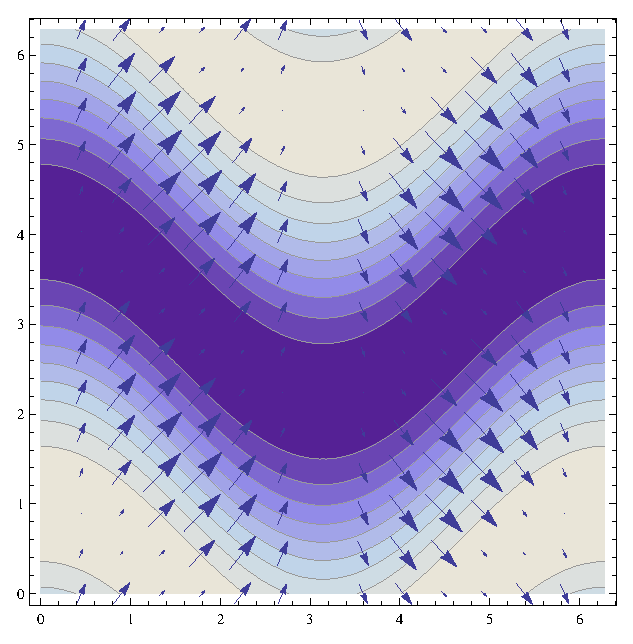
\includegraphics[scale=0.5]{figure-TM-field-components}}
\subfigure[$\mathbf{E_{\hat{n}}}$ for $\hat{\mathbf{y}}$ polarised light]{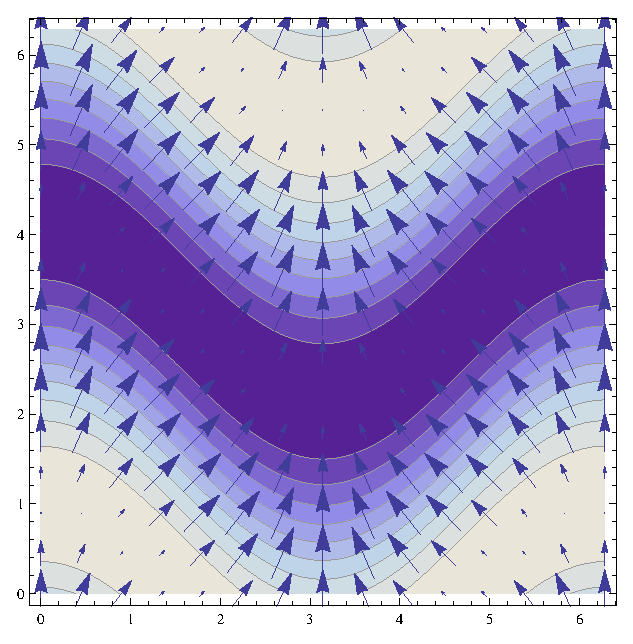
\includegraphics[scale=0.5]{figure-TE-field-components}}
\end{center}
\caption[The surface normal components of electric field vector for TM and TE polarised light projected on a contour of the zigzag surface profile.]{The surface normal components of electric field vector for (a) TM and (b) TE polarised light (arrows) projected on a contour of the zigzag surface profile. The contour plot amplitude ranges from 1 (white) to -1 (blue). \label{fig:zzEnormal}}
\end{figure}

We can now examine the functional form of the allowed normal electric field in the propagation direction for a SPP. The components, $E_{TE}$ and $E_{TM}$, of the electric field normal to the surface, lying along the direction of propagation (the $\mathbf{\hat{x}}$ direction) and integrated over $y$ for the two polarisation cases are found to be,
\begin{align}
E_{TM}& = -\frac{4\pi \sin^2{(x)}}{\cos{(2x)-3}}\label{eq:etm}\\
E_{TE} &= -\frac{4\pi \sin{(x)}}{\cos{(2x)-3}}\label{eq:ete}
\end{align}
Both $E_{TE}$ and $E_{TM}$ are non-zero, so we may conclude that either polarisation may induce surface charge and possibly excite SPPs. Plots of $E_{TM}$ and $E_{TE}$ in figure \ref{fig:e-te-and-e-tm} show that the electric field vector normal to the surface varies spatially twice as fast for the TM case as for the TE case. This leads to the conclusion that the wavevector of a TM-coupled SPP is required to be twice that of the TE-coupled case.
\begin{figure}
\begin{center}
% Created by tikzDevice version 0.6.2-92-0ad2792 on 2012-09-27 16:51:00
% !TEX encoding = UTF-8 Unicode
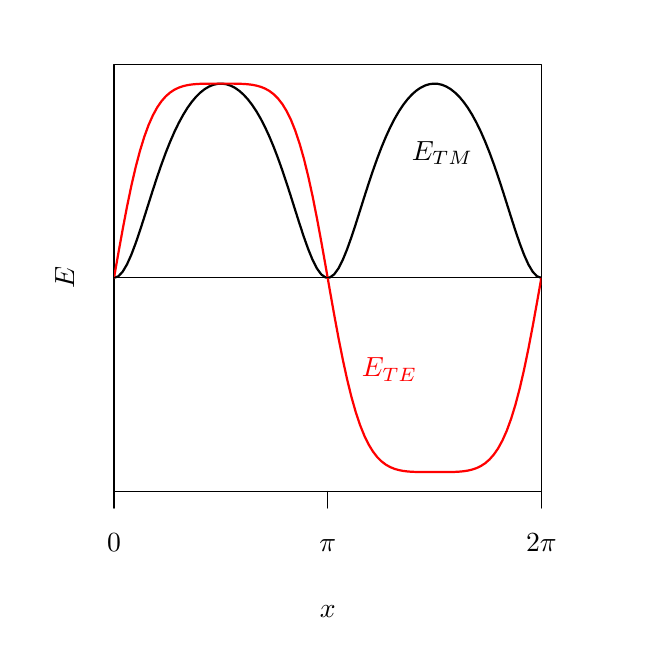
\begin{tikzpicture}[x=1pt,y=1pt]
\definecolor[named]{fillColor}{rgb}{1.00,1.00,1.00}
\path[use as bounding box,fill=fillColor,fill opacity=0.00] (0,0) rectangle (216.81,216.81);
\begin{scope}
\path[clip] (  0.00,  0.00) rectangle (216.81,216.81);
\definecolor[named]{drawColor}{rgb}{0.00,0.00,0.00}

\path[draw=drawColor,line width= 0.4pt,line join=round,line cap=round] ( 31.20, 49.20) --
	(185.61, 49.20) --
	(185.61,203.61) --
	( 31.20,203.61) --
	( 31.20, 49.20);
\end{scope}
\begin{scope}
\path[clip] (  0.00,  0.00) rectangle (216.81,216.81);
\definecolor[named]{drawColor}{rgb}{0.00,0.00,0.00}

\node[text=drawColor,anchor=base,inner sep=0pt, outer sep=0pt, scale=  1.00] at (108.41,  3.60) {$x$};
\end{scope}
\begin{scope}
\path[clip] (  0.00,  0.00) rectangle (216.81,216.81);
\definecolor[named]{drawColor}{rgb}{0.00,0.00,0.00}

\node[text=drawColor,rotate= 90.00,anchor=base,inner sep=0pt, outer sep=0pt, scale=  1.00] at ( 16.80,126.41) {$E$};
\end{scope}
\begin{scope}
\path[clip] ( 31.20, 49.20) rectangle (185.61,203.61);
\definecolor[named]{drawColor}{rgb}{0.00,0.00,0.00}

\path[draw=drawColor,line width= 0.8pt,line join=round,line cap=round] ( 31.20,126.41) --
	( 32.76,126.97) --
	( 34.32,128.62) --
	( 35.88,131.26) --
	( 37.44,134.73) --
	( 39.00,138.86) --
	( 40.56,143.44) --
	( 42.12,148.29) --
	( 43.68,153.24) --
	( 45.24,158.15) --
	( 46.80,162.92) --
	( 48.36,167.45) --
	( 49.92,171.69) --
	( 51.48,175.60) --
	( 53.04,179.18) --
	( 54.60,182.40) --
	( 56.16,185.26) --
	( 57.71,187.78) --
	( 59.27,189.96) --
	( 60.83,191.82) --
	( 62.39,193.35) --
	( 63.95,194.59) --
	( 65.51,195.52) --
	( 67.07,196.16) --
	( 68.63,196.51) --
	( 70.19,196.58) --
	( 71.75,196.37) --
	( 73.31,195.87) --
	( 74.87,195.09) --
	( 76.43,194.01) --
	( 77.99,192.63) --
	( 79.55,190.93) --
	( 81.11,188.91) --
	( 82.67,186.56) --
	( 84.23,183.87) --
	( 85.79,180.83) --
	( 87.35,177.43) --
	( 88.91,173.69) --
	( 90.47,169.61) --
	( 92.03,165.21) --
	( 93.59,160.56) --
	( 95.15,155.71) --
	( 96.71,150.76) --
	( 98.27,145.84) --
	( 99.83,141.11) --
	(101.39,136.73) --
	(102.95,132.90) --
	(104.51,129.82) --
	(106.07,127.66) --
	(107.63,126.55) --
	(109.18,126.55) --
	(110.74,127.66) --
	(112.30,129.82) --
	(113.86,132.90) --
	(115.42,136.73) --
	(116.98,141.11) --
	(118.54,145.84) --
	(120.10,150.76) --
	(121.66,155.71) --
	(123.22,160.56) --
	(124.78,165.21) --
	(126.34,169.61) --
	(127.90,173.69) --
	(129.46,177.43) --
	(131.02,180.83) --
	(132.58,183.87) --
	(134.14,186.56) --
	(135.70,188.91) --
	(137.26,190.93) --
	(138.82,192.63) --
	(140.38,194.01) --
	(141.94,195.09) --
	(143.50,195.87) --
	(145.06,196.37) --
	(146.62,196.58) --
	(148.18,196.51) --
	(149.74,196.16) --
	(151.30,195.52) --
	(152.86,194.59) --
	(154.42,193.35) --
	(155.98,191.82) --
	(157.54,189.96) --
	(159.10,187.78) --
	(160.65,185.26) --
	(162.21,182.40) --
	(163.77,179.18) --
	(165.33,175.60) --
	(166.89,171.69) --
	(168.45,167.45) --
	(170.01,162.92) --
	(171.57,158.15) --
	(173.13,153.24) --
	(174.69,148.29) --
	(176.25,143.44) --
	(177.81,138.86) --
	(179.37,134.73) --
	(180.93,131.26) --
	(182.49,128.62) --
	(184.05,126.97) --
	(185.61,126.41);
\definecolor[named]{drawColor}{rgb}{1.00,0.00,0.00}

\path[draw=drawColor,line width= 0.8pt,line join=round,line cap=round] ( 31.20,126.41) --
	( 32.76,135.27) --
	( 34.32,143.89) --
	( 35.88,152.05) --
	( 37.44,159.57) --
	( 39.00,166.32) --
	( 40.56,172.24) --
	( 42.12,177.33) --
	( 43.68,181.61) --
	( 45.24,185.13) --
	( 46.80,187.99) --
	( 48.36,190.25) --
	( 49.92,192.02) --
	( 51.48,193.38) --
	( 53.04,194.40) --
	( 54.60,195.14) --
	( 56.16,195.67) --
	( 57.71,196.04) --
	( 59.27,196.28) --
	( 60.83,196.43) --
	( 62.39,196.52) --
	( 63.95,196.56) --
	( 65.51,196.58) --
	( 67.07,196.59) --
	( 68.63,196.59) --
	( 70.19,196.59) --
	( 71.75,196.59) --
	( 73.31,196.59) --
	( 74.87,196.58) --
	( 76.43,196.54) --
	( 77.99,196.48) --
	( 79.55,196.36) --
	( 81.11,196.17) --
	( 82.67,195.87) --
	( 84.23,195.43) --
	( 85.79,194.80) --
	( 87.35,193.93) --
	( 88.91,192.75) --
	( 90.47,191.20) --
	( 92.03,189.19) --
	( 93.59,186.64) --
	( 95.15,183.46) --
	( 96.71,179.57) --
	( 98.27,174.89) --
	( 99.83,169.39) --
	(101.39,163.04) --
	(102.95,155.90) --
	(104.51,148.04) --
	(106.07,139.63) --
	(107.63,130.85) --
	(109.18,121.96) --
	(110.74,113.18) --
	(112.30,104.77) --
	(113.86, 96.91) --
	(115.42, 89.77) --
	(116.98, 83.42) --
	(118.54, 77.92) --
	(120.10, 73.24) --
	(121.66, 69.35) --
	(123.22, 66.17) --
	(124.78, 63.62) --
	(126.34, 61.61) --
	(127.90, 60.06) --
	(129.46, 58.88) --
	(131.02, 58.01) --
	(132.58, 57.38) --
	(134.14, 56.94) --
	(135.70, 56.64) --
	(137.26, 56.45) --
	(138.82, 56.33) --
	(140.38, 56.27) --
	(141.94, 56.23) --
	(143.50, 56.22) --
	(145.06, 56.22) --
	(146.62, 56.22) --
	(148.18, 56.22) --
	(149.74, 56.22) --
	(151.30, 56.23) --
	(152.86, 56.25) --
	(154.42, 56.29) --
	(155.98, 56.38) --
	(157.54, 56.53) --
	(159.10, 56.77) --
	(160.65, 57.14) --
	(162.21, 57.67) --
	(163.77, 58.41) --
	(165.33, 59.43) --
	(166.89, 60.79) --
	(168.45, 62.56) --
	(170.01, 64.82) --
	(171.57, 67.68) --
	(173.13, 71.20) --
	(174.69, 75.48) --
	(176.25, 80.57) --
	(177.81, 86.49) --
	(179.37, 93.24) --
	(180.93,100.76) --
	(182.49,108.92) --
	(184.05,117.54) --
	(185.61,126.40);
\definecolor[named]{drawColor}{rgb}{0.00,0.00,0.00}

\path[draw=drawColor,line width= 0.4pt,line join=round,line cap=round] ( 31.20,126.41) --
	( 32.76,126.41) --
	( 34.32,126.41) --
	( 35.88,126.41) --
	( 37.44,126.41) --
	( 39.00,126.41) --
	( 40.56,126.41) --
	( 42.12,126.41) --
	( 43.68,126.41) --
	( 45.24,126.41) --
	( 46.80,126.41) --
	( 48.36,126.41) --
	( 49.92,126.41) --
	( 51.48,126.41) --
	( 53.04,126.41) --
	( 54.60,126.41) --
	( 56.16,126.41) --
	( 57.71,126.41) --
	( 59.27,126.41) --
	( 60.83,126.41) --
	( 62.39,126.41) --
	( 63.95,126.41) --
	( 65.51,126.41) --
	( 67.07,126.41) --
	( 68.63,126.41) --
	( 70.19,126.41) --
	( 71.75,126.41) --
	( 73.31,126.41) --
	( 74.87,126.41) --
	( 76.43,126.41) --
	( 77.99,126.41) --
	( 79.55,126.41) --
	( 81.11,126.41) --
	( 82.67,126.41) --
	( 84.23,126.41) --
	( 85.79,126.41) --
	( 87.35,126.41) --
	( 88.91,126.41) --
	( 90.47,126.41) --
	( 92.03,126.41) --
	( 93.59,126.41) --
	( 95.15,126.41) --
	( 96.71,126.41) --
	( 98.27,126.41) --
	( 99.83,126.41) --
	(101.39,126.41) --
	(102.95,126.41) --
	(104.51,126.41) --
	(106.07,126.41) --
	(107.63,126.41) --
	(109.18,126.41) --
	(110.74,126.41) --
	(112.30,126.41) --
	(113.86,126.41) --
	(115.42,126.41) --
	(116.98,126.41) --
	(118.54,126.41) --
	(120.10,126.41) --
	(121.66,126.41) --
	(123.22,126.41) --
	(124.78,126.41) --
	(126.34,126.41) --
	(127.90,126.41) --
	(129.46,126.41) --
	(131.02,126.41) --
	(132.58,126.41) --
	(134.14,126.41) --
	(135.70,126.41) --
	(137.26,126.41) --
	(138.82,126.41) --
	(140.38,126.41) --
	(141.94,126.41) --
	(143.50,126.41) --
	(145.06,126.41) --
	(146.62,126.41) --
	(148.18,126.41) --
	(149.74,126.41) --
	(151.30,126.41) --
	(152.86,126.41) --
	(154.42,126.41) --
	(155.98,126.41) --
	(157.54,126.41) --
	(159.10,126.41) --
	(160.65,126.41) --
	(162.21,126.41) --
	(163.77,126.41) --
	(165.33,126.41) --
	(166.89,126.41) --
	(168.45,126.41) --
	(170.01,126.41) --
	(171.57,126.41) --
	(173.13,126.41) --
	(174.69,126.41) --
	(176.25,126.41) --
	(177.81,126.41) --
	(179.37,126.41) --
	(180.93,126.41) --
	(182.49,126.41) --
	(184.05,126.41) --
	(185.61,126.41);
\definecolor[named]{drawColor}{rgb}{1.00,0.00,0.00}

\node[text=drawColor,anchor=base west,inner sep=0pt, outer sep=0pt, scale=  1.00] at (120.76, 90.60) {$E_{TE}$};
\definecolor[named]{drawColor}{rgb}{0.00,0.00,0.00}

\node[text=drawColor,anchor=base east,inner sep=0pt, outer sep=0pt, scale=  1.00] at (160.85,168.79) {$E_{TM}$};
\end{scope}
\begin{scope}
\path[clip] (  0.00,  0.00) rectangle (216.81,216.81);
\definecolor[named]{drawColor}{rgb}{0.00,0.00,0.00}

\path[draw=drawColor,line width= 0.4pt,line join=round,line cap=round] ( 31.20, 49.20) -- (185.61, 49.20);

\path[draw=drawColor,line width= 0.4pt,line join=round,line cap=round] ( 31.20, 49.20) -- ( 31.20, 43.20);

\path[draw=drawColor,line width= 0.4pt,line join=round,line cap=round] (108.41, 49.20) -- (108.41, 43.20);

\path[draw=drawColor,line width= 0.4pt,line join=round,line cap=round] (185.61, 49.20) -- (185.61, 43.20);

\node[text=drawColor,anchor=base,inner sep=0pt, outer sep=0pt, scale=  1.00] at ( 31.20, 27.60) {0};

\node[text=drawColor,anchor=base,inner sep=0pt, outer sep=0pt, scale=  1.00] at (108.41, 27.60) {$\pi$};

\node[text=drawColor,anchor=base,inner sep=0pt, outer sep=0pt, scale=  1.00] at (185.61, 27.60) {$2\pi$};
\end{scope}
\end{tikzpicture}

\caption{The magnitude of the surface normal electric field in the x-direction for TM and TE polarisations.\label{fig:e-te-and-e-tm}}
\end{center}
\end{figure}
By expanding both these expressions as a Fourier sum in $x$, we may express the $E_{TM}$ and $E_{TE}$ as a sum of plane-waves. It is possible then to find which in-plane wavevectors of incident light are required to match these field profiles. Doing so yields,
\begin{align}
E_{TE}=&\;\!\!\!\!\!\sum\limits_{n=1,3,5,...}^\infty \!\!\!\!\!a_n\cos{(nx)}\label{eq:zz-tmcouping}\\
E_{TM}=&\;a_0+\!\!\!\!\!\displaystyle\sum\limits_{n=2,4,6,...}^\infty \!\!\!\!\!b_n\sin{(nx)}\label{eq:zz-tecoupling}
\end{align}
where $a_n$ and $b_n$ are the Fourier series coefficients. For incident light to match $E_{TE}$ requires a series of only odd-ordered terms, while $E_{TM}$ requires a series of only even-ordered terms. Diffracted fields at the surface will contain both odd and even wavevector components. Equations \ref{eq:zz-tmcouping} and \ref{eq:zz-tecoupling} predict that TE polarised light will provide a suitable electric field distribution to enable the excitation of SPPs via only odd-ordered diffracted orders, while TM polarised light will excite SPPs only via even-ordered diffracted orders.  This concept will be discussed again with reference to the experimental and modelled results in sections \ref{sec:TEexciatation} and \ref{sec:TMexciatation}.

We can visualise these coupling conditions in a simplistic diagrammatic way, shown in in figure \ref{fig:coupling-cartoon}.
\begin{figure}
\begin{center}
% Created by tikzDevice version 0.6.2-92-0ad2792 on 2012-12-18 10:42:07
% !TEX encoding = UTF-8 Unicode
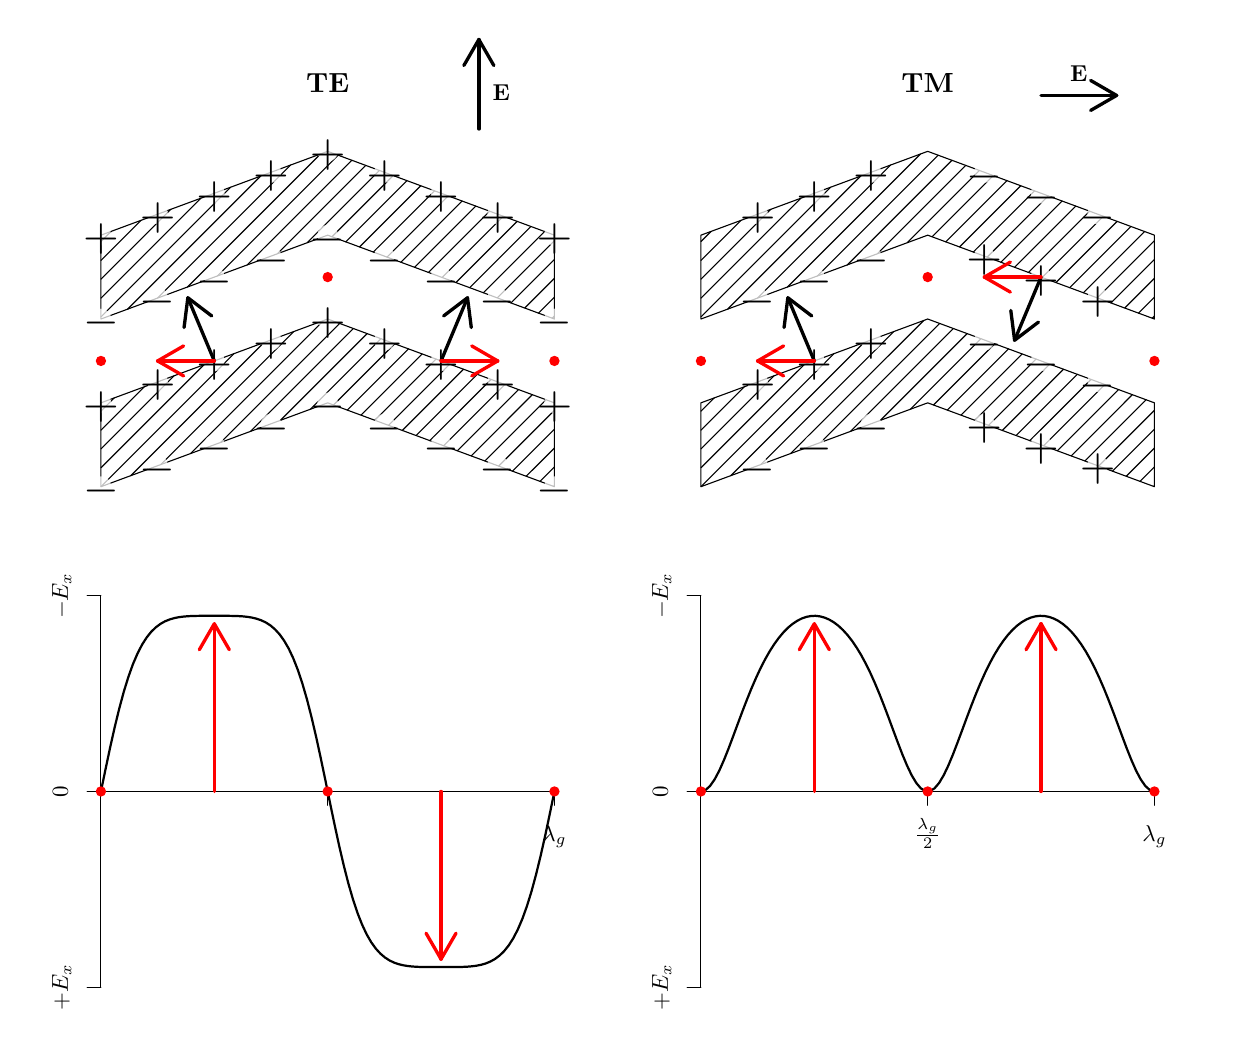
\begin{tikzpicture}[x=1pt,y=1pt]
\definecolor[named]{fillColor}{rgb}{1.00,1.00,1.00}
\path[use as bounding box,fill=fillColor,fill opacity=0.00] (0,0) rectangle (433.62,361.35);
\begin{scope}
\path[clip] (  0.00,180.67) rectangle (216.81,361.35);
\definecolor[named]{drawColor}{rgb}{0.00,0.00,0.00}

\node[text=drawColor,anchor=base,inner sep=0pt, outer sep=0pt, scale=  0.83] at (108.41,152.79) {x};

\path[draw=drawColor,line width= 0.4pt,line join=round,line cap=round] ( 26.47,222.74) -- ( 31.30,227.56);

\path[draw=drawColor,line width= 0.4pt,line join=round,line cap=round] ( 26.47,215.92) -- ( 42.11,231.56);

\path[draw=drawColor,line width= 0.4pt,line join=round,line cap=round] ( 26.47,209.11) -- ( 52.92,235.56);

\path[draw=drawColor,line width= 0.4pt,line join=round,line cap=round] ( 26.47,202.30) -- ( 63.73,239.55);

\path[draw=drawColor,line width= 0.4pt,line join=round,line cap=round] ( 26.47,195.48) -- ( 74.54,243.55);

\path[draw=drawColor,line width= 0.4pt,line join=round,line cap=round] ( 37.29,199.48) -- ( 85.36,247.55);

\path[draw=drawColor,line width= 0.4pt,line join=round,line cap=round] ( 48.10,203.48) -- ( 96.17,251.55);

\path[draw=drawColor,line width= 0.4pt,line join=round,line cap=round] ( 58.91,207.48) -- (106.98,255.54);

\path[draw=drawColor,line width= 0.4pt,line join=round,line cap=round] ( 69.72,211.47) -- (112.72,254.48);

\path[draw=drawColor,line width= 0.4pt,line join=round,line cap=round] ( 80.53,215.47) -- (117.70,252.64);

\path[draw=drawColor,line width= 0.4pt,line join=round,line cap=round] ( 91.34,219.47) -- (122.67,250.80);

\path[draw=drawColor,line width= 0.4pt,line join=round,line cap=round] (102.15,223.47) -- (127.65,248.96);

\path[draw=drawColor,line width= 0.4pt,line join=round,line cap=round] (110.50,225.00) -- (132.62,247.12);

\path[draw=drawColor,line width= 0.4pt,line join=round,line cap=round] (115.48,223.16) -- (137.59,245.28);

\path[draw=drawColor,line width= 0.4pt,line join=round,line cap=round] (120.45,221.32) -- (142.57,243.44);

\path[draw=drawColor,line width= 0.4pt,line join=round,line cap=round] (125.43,219.48) -- (147.54,241.60);

\path[draw=drawColor,line width= 0.4pt,line join=round,line cap=round] (130.40,217.64) -- (152.52,239.76);

\path[draw=drawColor,line width= 0.4pt,line join=round,line cap=round] (135.37,215.80) -- (157.49,237.92);

\path[draw=drawColor,line width= 0.4pt,line join=round,line cap=round] (140.35,213.97) -- (162.47,236.08);

\path[draw=drawColor,line width= 0.4pt,line join=round,line cap=round] (145.32,212.13) -- (167.44,234.24);

\path[draw=drawColor,line width= 0.4pt,line join=round,line cap=round] (150.30,210.29) -- (172.41,232.40);

\path[draw=drawColor,line width= 0.4pt,line join=round,line cap=round] (155.27,208.45) -- (177.39,230.56);

\path[draw=drawColor,line width= 0.4pt,line join=round,line cap=round] (160.25,206.61) -- (182.36,228.73);

\path[draw=drawColor,line width= 0.4pt,line join=round,line cap=round] (165.22,204.77) -- (187.34,226.89);

\path[draw=drawColor,line width= 0.4pt,line join=round,line cap=round] (170.20,202.93) -- (190.34,223.07);

\path[draw=drawColor,line width= 0.4pt,line join=round,line cap=round] (175.17,201.09) -- (190.34,216.26);

\path[draw=drawColor,line width= 0.4pt,line join=round,line cap=round] (180.14,199.25) -- (190.34,209.44);

\path[draw=drawColor,line width= 0.4pt,line join=round,line cap=round] (185.12,197.41) -- (190.34,202.63);

\path[draw=drawColor,line width= 0.4pt,line join=round,line cap=round] (190.09,195.57) -- (190.34,195.81);

\path[draw=drawColor,line width= 0.4pt,line join=round,line cap=round] ( 26.47,195.48) --
	( 26.47,225.78) --
	(108.41,256.07) --
	(190.34,225.78) --
	(190.34,195.48) --
	(108.41,225.78) --
	( 26.47,195.48);

\path[draw=drawColor,line width= 0.4pt,line join=round,line cap=round] ( 26.47,284.06) -- ( 30.14,287.72);

\path[draw=drawColor,line width= 0.4pt,line join=round,line cap=round] ( 26.47,277.25) -- ( 40.95,291.72);

\path[draw=drawColor,line width= 0.4pt,line join=round,line cap=round] ( 26.47,270.43) -- ( 51.76,295.72);

\path[draw=drawColor,line width= 0.4pt,line join=round,line cap=round] ( 26.47,263.62) -- ( 62.57,299.71);

\path[draw=drawColor,line width= 0.4pt,line join=round,line cap=round] ( 26.47,256.81) -- ( 73.38,303.71);

\path[draw=drawColor,line width= 0.4pt,line join=round,line cap=round] ( 36.12,259.64) -- ( 84.19,307.71);

\path[draw=drawColor,line width= 0.4pt,line join=round,line cap=round] ( 46.93,263.64) -- ( 95.00,311.71);

\path[draw=drawColor,line width= 0.4pt,line join=round,line cap=round] ( 57.75,267.64) -- (105.82,315.71);

\path[draw=drawColor,line width= 0.4pt,line join=round,line cap=round] ( 68.56,271.63) -- (112.19,315.26);

\path[draw=drawColor,line width= 0.4pt,line join=round,line cap=round] ( 79.37,275.63) -- (117.16,313.42);

\path[draw=drawColor,line width= 0.4pt,line join=round,line cap=round] ( 90.18,279.63) -- (122.14,311.59);

\path[draw=drawColor,line width= 0.4pt,line join=round,line cap=round] (100.99,283.63) -- (127.11,309.75);

\path[draw=drawColor,line width= 0.4pt,line join=round,line cap=round] (109.97,285.79) -- (132.09,307.91);

\path[draw=drawColor,line width= 0.4pt,line join=round,line cap=round] (114.94,283.95) -- (137.06,306.07);

\path[draw=drawColor,line width= 0.4pt,line join=round,line cap=round] (119.92,282.11) -- (142.03,304.23);

\path[draw=drawColor,line width= 0.4pt,line join=round,line cap=round] (124.89,280.27) -- (147.01,302.39);

\path[draw=drawColor,line width= 0.4pt,line join=round,line cap=round] (129.87,278.43) -- (151.98,300.55);

\path[draw=drawColor,line width= 0.4pt,line join=round,line cap=round] (134.84,276.59) -- (156.96,298.71);

\path[draw=drawColor,line width= 0.4pt,line join=round,line cap=round] (139.81,274.75) -- (161.93,296.87);

\path[draw=drawColor,line width= 0.4pt,line join=round,line cap=round] (144.79,272.91) -- (166.91,295.03);

\path[draw=drawColor,line width= 0.4pt,line join=round,line cap=round] (149.76,271.07) -- (171.88,293.19);

\path[draw=drawColor,line width= 0.4pt,line join=round,line cap=round] (154.74,269.24) -- (176.85,291.35);

\path[draw=drawColor,line width= 0.4pt,line join=round,line cap=round] (159.71,267.40) -- (181.83,289.51);

\path[draw=drawColor,line width= 0.4pt,line join=round,line cap=round] (164.69,265.56) -- (186.80,287.67);

\path[draw=drawColor,line width= 0.4pt,line join=round,line cap=round] (169.66,263.72) -- (190.34,284.39);

\path[draw=drawColor,line width= 0.4pt,line join=round,line cap=round] (174.63,261.88) -- (190.34,277.58);

\path[draw=drawColor,line width= 0.4pt,line join=round,line cap=round] (179.61,260.04) -- (190.34,270.77);

\path[draw=drawColor,line width= 0.4pt,line join=round,line cap=round] (184.58,258.20) -- (190.34,263.95);

\path[draw=drawColor,line width= 0.4pt,line join=round,line cap=round] (189.56,256.36) -- (190.34,257.14);

\path[draw=drawColor,line width= 0.4pt,line join=round,line cap=round] ( 26.47,256.07) --
	( 26.47,286.37) --
	(108.41,316.66) --
	(190.34,286.37) --
	(190.34,256.07) --
	(108.41,286.37) --
	( 26.47,256.07);
\definecolor[named]{fillColor}{rgb}{1.00,1.00,1.00}

\path[fill=fillColor,fill opacity=0.75] ( 26.47,225.78) circle (  3.73);

\path[fill=fillColor,fill opacity=0.75] ( 46.96,233.45) circle (  3.73);

\path[fill=fillColor,fill opacity=0.75] ( 67.44,240.92) circle (  3.73);

\path[fill=fillColor,fill opacity=0.75] ( 87.92,248.40) circle (  3.73);

\path[fill=fillColor,fill opacity=0.75] (108.41,256.07) circle (  3.73);

\path[fill=fillColor,fill opacity=0.75] (128.89,248.40) circle (  3.73);

\path[fill=fillColor,fill opacity=0.75] (149.37,240.92) circle (  3.73);

\path[fill=fillColor,fill opacity=0.75] (169.85,233.45) circle (  3.73);

\path[fill=fillColor,fill opacity=0.75] (190.34,225.78) circle (  3.73);

\path[fill=fillColor,fill opacity=0.75] ( 26.47,256.07) circle (  3.73);

\path[fill=fillColor,fill opacity=0.75] ( 46.96,263.75) circle (  3.73);

\path[fill=fillColor,fill opacity=0.75] ( 67.44,271.22) circle (  3.73);

\path[fill=fillColor,fill opacity=0.75] ( 87.92,278.69) circle (  3.73);

\path[fill=fillColor,fill opacity=0.75] (108.41,286.37) circle (  3.73);

\path[fill=fillColor,fill opacity=0.75] (128.89,278.69) circle (  3.73);

\path[fill=fillColor,fill opacity=0.75] (149.37,271.22) circle (  3.73);

\path[fill=fillColor,fill opacity=0.75] (169.85,263.75) circle (  3.73);

\path[fill=fillColor,fill opacity=0.75] (190.34,256.07) circle (  3.73);

\path[fill=fillColor,fill opacity=0.75] ( 26.47,286.37) circle (  3.73);

\path[fill=fillColor,fill opacity=0.75] ( 46.96,294.04) circle (  3.73);

\path[fill=fillColor,fill opacity=0.75] ( 67.44,301.52) circle (  3.73);

\path[fill=fillColor,fill opacity=0.75] ( 87.92,308.99) circle (  3.73);

\path[fill=fillColor,fill opacity=0.75] (108.41,316.66) circle (  3.73);

\path[fill=fillColor,fill opacity=0.75] (128.89,308.99) circle (  3.73);

\path[fill=fillColor,fill opacity=0.75] (149.37,301.52) circle (  3.73);

\path[fill=fillColor,fill opacity=0.75] (169.85,294.04) circle (  3.73);

\path[fill=fillColor,fill opacity=0.75] (190.34,286.37) circle (  3.73);

\path[fill=fillColor,fill opacity=0.75] ( 26.47,195.48) circle (  3.73);

\path[fill=fillColor,fill opacity=0.75] ( 46.96,203.16) circle (  3.73);

\path[fill=fillColor,fill opacity=0.75] ( 67.44,210.63) circle (  3.73);

\path[fill=fillColor,fill opacity=0.75] ( 87.92,218.10) circle (  3.73);

\path[fill=fillColor,fill opacity=0.75] (108.41,225.78) circle (  3.73);

\path[fill=fillColor,fill opacity=0.75] (128.89,218.10) circle (  3.73);

\path[fill=fillColor,fill opacity=0.75] (149.37,210.63) circle (  3.73);

\path[fill=fillColor,fill opacity=0.75] (169.85,203.16) circle (  3.73);

\path[fill=fillColor,fill opacity=0.75] (190.34,195.48) circle (  3.73);

\node[text=drawColor,anchor=base,inner sep=0pt, outer sep=0pt, scale=  1.66] at ( 26.47,220.25) {$+$};

\node[text=drawColor,anchor=base,inner sep=0pt, outer sep=0pt, scale=  1.66] at ( 46.96,227.92) {$+$};

\node[text=drawColor,anchor=base,inner sep=0pt, outer sep=0pt, scale=  1.66] at ( 67.44,235.39) {$+$};

\node[text=drawColor,anchor=base,inner sep=0pt, outer sep=0pt, scale=  1.66] at ( 87.92,242.87) {$+$};

\node[text=drawColor,anchor=base,inner sep=0pt, outer sep=0pt, scale=  1.66] at (108.41,250.54) {$+$};

\node[text=drawColor,anchor=base,inner sep=0pt, outer sep=0pt, scale=  1.66] at (128.89,242.87) {$+$};

\node[text=drawColor,anchor=base,inner sep=0pt, outer sep=0pt, scale=  1.66] at (149.37,235.39) {$+$};

\node[text=drawColor,anchor=base,inner sep=0pt, outer sep=0pt, scale=  1.66] at (169.85,227.92) {$+$};

\node[text=drawColor,anchor=base,inner sep=0pt, outer sep=0pt, scale=  1.66] at (190.34,220.25) {$+$};

\node[text=drawColor,anchor=base,inner sep=0pt, outer sep=0pt, scale=  1.66] at ( 26.47,250.31) {$-$};

\node[text=drawColor,anchor=base,inner sep=0pt, outer sep=0pt, scale=  1.66] at ( 46.96,257.98) {$-$};

\node[text=drawColor,anchor=base,inner sep=0pt, outer sep=0pt, scale=  1.66] at ( 67.44,265.46) {$-$};

\node[text=drawColor,anchor=base,inner sep=0pt, outer sep=0pt, scale=  1.66] at ( 87.92,272.93) {$-$};

\node[text=drawColor,anchor=base,inner sep=0pt, outer sep=0pt, scale=  1.66] at (108.41,280.61) {$-$};

\node[text=drawColor,anchor=base,inner sep=0pt, outer sep=0pt, scale=  1.66] at (128.89,272.93) {$-$};

\node[text=drawColor,anchor=base,inner sep=0pt, outer sep=0pt, scale=  1.66] at (149.37,265.46) {$-$};

\node[text=drawColor,anchor=base,inner sep=0pt, outer sep=0pt, scale=  1.66] at (169.85,257.98) {$-$};

\node[text=drawColor,anchor=base,inner sep=0pt, outer sep=0pt, scale=  1.66] at (190.34,250.31) {$-$};

\node[text=drawColor,anchor=base,inner sep=0pt, outer sep=0pt, scale=  1.66] at ( 26.47,280.84) {$+$};

\node[text=drawColor,anchor=base,inner sep=0pt, outer sep=0pt, scale=  1.66] at ( 46.96,288.51) {$+$};

\node[text=drawColor,anchor=base,inner sep=0pt, outer sep=0pt, scale=  1.66] at ( 67.44,295.98) {$+$};

\node[text=drawColor,anchor=base,inner sep=0pt, outer sep=0pt, scale=  1.66] at ( 87.92,303.46) {$+$};

\node[text=drawColor,anchor=base,inner sep=0pt, outer sep=0pt, scale=  1.66] at (108.41,311.13) {$+$};

\node[text=drawColor,anchor=base,inner sep=0pt, outer sep=0pt, scale=  1.66] at (128.89,303.46) {$+$};

\node[text=drawColor,anchor=base,inner sep=0pt, outer sep=0pt, scale=  1.66] at (149.37,295.98) {$+$};

\node[text=drawColor,anchor=base,inner sep=0pt, outer sep=0pt, scale=  1.66] at (169.85,288.51) {$+$};

\node[text=drawColor,anchor=base,inner sep=0pt, outer sep=0pt, scale=  1.66] at (190.34,280.84) {$+$};

\node[text=drawColor,anchor=base,inner sep=0pt, outer sep=0pt, scale=  1.66] at ( 26.47,189.72) {$-$};

\node[text=drawColor,anchor=base,inner sep=0pt, outer sep=0pt, scale=  1.66] at ( 46.96,197.39) {$-$};

\node[text=drawColor,anchor=base,inner sep=0pt, outer sep=0pt, scale=  1.66] at ( 67.44,204.87) {$-$};

\node[text=drawColor,anchor=base,inner sep=0pt, outer sep=0pt, scale=  1.66] at ( 87.92,212.34) {$-$};

\node[text=drawColor,anchor=base,inner sep=0pt, outer sep=0pt, scale=  1.66] at (108.41,220.01) {$-$};

\node[text=drawColor,anchor=base,inner sep=0pt, outer sep=0pt, scale=  1.66] at (128.89,212.34) {$-$};

\node[text=drawColor,anchor=base,inner sep=0pt, outer sep=0pt, scale=  1.66] at (149.37,204.87) {$-$};

\node[text=drawColor,anchor=base,inner sep=0pt, outer sep=0pt, scale=  1.66] at (169.85,197.39) {$-$};

\node[text=drawColor,anchor=base,inner sep=0pt, outer sep=0pt, scale=  1.66] at (190.34,189.72) {$-$};

\path[draw=drawColor,line width= 1.2pt,line join=round,line cap=round] (163.03,324.74) -- (163.03,357.06);

\path[draw=drawColor,line width= 1.2pt,line join=round,line cap=round] (168.45,347.67) --
	(163.03,357.06) --
	(157.61,347.67);

\node[text=drawColor,anchor=base west,inner sep=0pt, outer sep=0pt, scale=  0.83] at (168.01,334.95) {$\mathbf{E}$};

\path[draw=drawColor,line width= 1.2pt,line join=round,line cap=round] ( 67.44,240.92) -- ( 57.88,263.75);

\path[draw=drawColor,line width= 1.2pt,line join=round,line cap=round] ( 66.51,257.18) --
	( 57.88,263.75) --
	( 56.51,252.99);

\path[draw=drawColor,line width= 1.2pt,line join=round,line cap=round] (149.37,240.92) -- (158.93,263.75);

\path[draw=drawColor,line width= 1.2pt,line join=round,line cap=round] (160.30,252.99) --
	(158.93,263.75) --
	(150.30,257.18);
\definecolor[named]{drawColor}{rgb}{1.00,0.00,0.00}

\path[draw=drawColor,line width= 1.2pt,line join=round,line cap=round] ( 67.44,240.92) -- ( 46.96,240.92);

\path[draw=drawColor,line width= 1.2pt,line join=round,line cap=round] ( 56.35,246.35) --
	( 46.96,240.92) --
	( 56.35,235.50);

\path[draw=drawColor,line width= 1.2pt,line join=round,line cap=round] (149.37,240.92) -- (169.85,240.92);

\path[draw=drawColor,line width= 1.2pt,line join=round,line cap=round] (160.46,235.50) --
	(169.85,240.92) --
	(160.46,246.35);
\definecolor[named]{fillColor}{rgb}{1.00,0.00,0.00}

\path[fill=fillColor] ( 26.47,240.92) circle (  1.87);

\path[fill=fillColor] (108.41,271.22) circle (  1.87);

\path[fill=fillColor] (190.34,240.92) circle (  1.87);
\definecolor[named]{drawColor}{rgb}{0.00,0.00,0.00}

\node[text=drawColor,anchor=base,inner sep=0pt, outer sep=0pt, scale=  1.00] at (108.41,337.99) {\bfseries TE};
\end{scope}
\begin{scope}
\path[clip] (216.81,180.67) rectangle (433.62,361.35);
\definecolor[named]{drawColor}{rgb}{0.00,0.00,0.00}

\path[draw=drawColor,line width= 0.4pt,line join=round,line cap=round] (243.28,222.74) -- (248.11,227.56);

\path[draw=drawColor,line width= 0.4pt,line join=round,line cap=round] (243.28,215.92) -- (258.92,231.56);

\path[draw=drawColor,line width= 0.4pt,line join=round,line cap=round] (243.28,209.11) -- (269.73,235.56);

\path[draw=drawColor,line width= 0.4pt,line join=round,line cap=round] (243.28,202.30) -- (280.54,239.55);

\path[draw=drawColor,line width= 0.4pt,line join=round,line cap=round] (243.28,195.48) -- (291.35,243.55);

\path[draw=drawColor,line width= 0.4pt,line join=round,line cap=round] (254.10,199.48) -- (302.17,247.55);

\path[draw=drawColor,line width= 0.4pt,line join=round,line cap=round] (264.91,203.48) -- (312.98,251.55);

\path[draw=drawColor,line width= 0.4pt,line join=round,line cap=round] (275.72,207.48) -- (323.79,255.54);

\path[draw=drawColor,line width= 0.4pt,line join=round,line cap=round] (286.53,211.47) -- (329.53,254.48);

\path[draw=drawColor,line width= 0.4pt,line join=round,line cap=round] (297.34,215.47) -- (334.51,252.64);

\path[draw=drawColor,line width= 0.4pt,line join=round,line cap=round] (308.15,219.47) -- (339.48,250.80);

\path[draw=drawColor,line width= 0.4pt,line join=round,line cap=round] (318.96,223.47) -- (344.46,248.96);

\path[draw=drawColor,line width= 0.4pt,line join=round,line cap=round] (327.31,225.00) -- (349.43,247.12);

\path[draw=drawColor,line width= 0.4pt,line join=round,line cap=round] (332.29,223.16) -- (354.40,245.28);

\path[draw=drawColor,line width= 0.4pt,line join=round,line cap=round] (337.26,221.32) -- (359.38,243.44);

\path[draw=drawColor,line width= 0.4pt,line join=round,line cap=round] (342.24,219.48) -- (364.35,241.60);

\path[draw=drawColor,line width= 0.4pt,line join=round,line cap=round] (347.21,217.64) -- (369.33,239.76);

\path[draw=drawColor,line width= 0.4pt,line join=round,line cap=round] (352.18,215.80) -- (374.30,237.92);

\path[draw=drawColor,line width= 0.4pt,line join=round,line cap=round] (357.16,213.97) -- (379.28,236.08);

\path[draw=drawColor,line width= 0.4pt,line join=round,line cap=round] (362.13,212.13) -- (384.25,234.24);

\path[draw=drawColor,line width= 0.4pt,line join=round,line cap=round] (367.11,210.29) -- (389.22,232.40);

\path[draw=drawColor,line width= 0.4pt,line join=round,line cap=round] (372.08,208.45) -- (394.20,230.56);

\path[draw=drawColor,line width= 0.4pt,line join=round,line cap=round] (377.06,206.61) -- (399.17,228.73);

\path[draw=drawColor,line width= 0.4pt,line join=round,line cap=round] (382.03,204.77) -- (404.15,226.89);

\path[draw=drawColor,line width= 0.4pt,line join=round,line cap=round] (387.01,202.93) -- (407.15,223.07);

\path[draw=drawColor,line width= 0.4pt,line join=round,line cap=round] (391.98,201.09) -- (407.15,216.26);

\path[draw=drawColor,line width= 0.4pt,line join=round,line cap=round] (396.95,199.25) -- (407.15,209.44);

\path[draw=drawColor,line width= 0.4pt,line join=round,line cap=round] (401.93,197.41) -- (407.15,202.63);

\path[draw=drawColor,line width= 0.4pt,line join=round,line cap=round] (406.90,195.57) -- (407.15,195.81);

\path[draw=drawColor,line width= 0.4pt,line join=round,line cap=round] (243.28,195.48) --
	(243.28,225.78) --
	(325.22,256.07) --
	(407.15,225.78) --
	(407.15,195.48) --
	(325.22,225.78) --
	(243.28,195.48);

\path[draw=drawColor,line width= 0.4pt,line join=round,line cap=round] (243.28,284.06) -- (246.95,287.72);

\path[draw=drawColor,line width= 0.4pt,line join=round,line cap=round] (243.28,277.25) -- (257.76,291.72);

\path[draw=drawColor,line width= 0.4pt,line join=round,line cap=round] (243.28,270.43) -- (268.57,295.72);

\path[draw=drawColor,line width= 0.4pt,line join=round,line cap=round] (243.28,263.62) -- (279.38,299.71);

\path[draw=drawColor,line width= 0.4pt,line join=round,line cap=round] (243.28,256.81) -- (290.19,303.71);

\path[draw=drawColor,line width= 0.4pt,line join=round,line cap=round] (252.93,259.64) -- (301.00,307.71);

\path[draw=drawColor,line width= 0.4pt,line join=round,line cap=round] (263.74,263.64) -- (311.81,311.71);

\path[draw=drawColor,line width= 0.4pt,line join=round,line cap=round] (274.56,267.64) -- (322.63,315.71);

\path[draw=drawColor,line width= 0.4pt,line join=round,line cap=round] (285.37,271.63) -- (329.00,315.26);

\path[draw=drawColor,line width= 0.4pt,line join=round,line cap=round] (296.18,275.63) -- (333.97,313.42);

\path[draw=drawColor,line width= 0.4pt,line join=round,line cap=round] (306.99,279.63) -- (338.95,311.59);

\path[draw=drawColor,line width= 0.4pt,line join=round,line cap=round] (317.80,283.63) -- (343.92,309.75);

\path[draw=drawColor,line width= 0.4pt,line join=round,line cap=round] (326.78,285.79) -- (348.90,307.91);

\path[draw=drawColor,line width= 0.4pt,line join=round,line cap=round] (331.75,283.95) -- (353.87,306.07);

\path[draw=drawColor,line width= 0.4pt,line join=round,line cap=round] (336.73,282.11) -- (358.84,304.23);

\path[draw=drawColor,line width= 0.4pt,line join=round,line cap=round] (341.70,280.27) -- (363.82,302.39);

\path[draw=drawColor,line width= 0.4pt,line join=round,line cap=round] (346.68,278.43) -- (368.79,300.55);

\path[draw=drawColor,line width= 0.4pt,line join=round,line cap=round] (351.65,276.59) -- (373.77,298.71);

\path[draw=drawColor,line width= 0.4pt,line join=round,line cap=round] (356.62,274.75) -- (378.74,296.87);

\path[draw=drawColor,line width= 0.4pt,line join=round,line cap=round] (361.60,272.91) -- (383.72,295.03);

\path[draw=drawColor,line width= 0.4pt,line join=round,line cap=round] (366.57,271.07) -- (388.69,293.19);

\path[draw=drawColor,line width= 0.4pt,line join=round,line cap=round] (371.55,269.24) -- (393.66,291.35);

\path[draw=drawColor,line width= 0.4pt,line join=round,line cap=round] (376.52,267.40) -- (398.64,289.51);

\path[draw=drawColor,line width= 0.4pt,line join=round,line cap=round] (381.50,265.56) -- (403.61,287.67);

\path[draw=drawColor,line width= 0.4pt,line join=round,line cap=round] (386.47,263.72) -- (407.15,284.39);

\path[draw=drawColor,line width= 0.4pt,line join=round,line cap=round] (391.44,261.88) -- (407.15,277.58);

\path[draw=drawColor,line width= 0.4pt,line join=round,line cap=round] (396.42,260.04) -- (407.15,270.77);

\path[draw=drawColor,line width= 0.4pt,line join=round,line cap=round] (401.39,258.20) -- (407.15,263.95);

\path[draw=drawColor,line width= 0.4pt,line join=round,line cap=round] (406.37,256.36) -- (407.15,257.14);

\path[draw=drawColor,line width= 0.4pt,line join=round,line cap=round] (243.28,256.07) --
	(243.28,286.37) --
	(325.22,316.66) --
	(407.15,286.37) --
	(407.15,256.07) --
	(325.22,286.37) --
	(243.28,256.07);
\definecolor[named]{fillColor}{rgb}{1.00,1.00,1.00}

\path[fill=fillColor,fill opacity=0.75] (263.77,233.45) circle (  3.73);

\path[fill=fillColor,fill opacity=0.75] (284.25,240.92) circle (  3.73);

\path[fill=fillColor,fill opacity=0.75] (304.73,248.40) circle (  3.73);

\path[fill=fillColor,fill opacity=0.75] (345.70,248.40) circle (  3.73);

\path[fill=fillColor,fill opacity=0.75] (366.18,240.92) circle (  3.73);

\path[fill=fillColor,fill opacity=0.75] (386.66,233.45) circle (  3.73);

\path[fill=fillColor,fill opacity=0.75] (263.77,263.75) circle (  3.73);

\path[fill=fillColor,fill opacity=0.75] (284.25,271.22) circle (  3.73);

\path[fill=fillColor,fill opacity=0.75] (304.73,278.69) circle (  3.73);

\path[fill=fillColor,fill opacity=0.75] (345.70,278.69) circle (  3.73);

\path[fill=fillColor,fill opacity=0.75] (366.18,271.22) circle (  3.73);

\path[fill=fillColor,fill opacity=0.75] (386.66,263.75) circle (  3.73);

\path[fill=fillColor,fill opacity=0.75] (263.77,294.04) circle (  3.73);

\path[fill=fillColor,fill opacity=0.75] (284.25,301.52) circle (  3.73);

\path[fill=fillColor,fill opacity=0.75] (304.73,308.99) circle (  3.73);

\path[fill=fillColor,fill opacity=0.75] (345.70,308.99) circle (  3.73);

\path[fill=fillColor,fill opacity=0.75] (366.18,301.52) circle (  3.73);

\path[fill=fillColor,fill opacity=0.75] (386.66,294.04) circle (  3.73);

\path[fill=fillColor,fill opacity=0.75] (263.77,203.16) circle (  3.73);

\path[fill=fillColor,fill opacity=0.75] (284.25,210.63) circle (  3.73);

\path[fill=fillColor,fill opacity=0.75] (304.73,218.10) circle (  3.73);

\path[fill=fillColor,fill opacity=0.75] (345.70,218.10) circle (  3.73);

\path[fill=fillColor,fill opacity=0.75] (366.18,210.63) circle (  3.73);

\path[fill=fillColor,fill opacity=0.75] (386.66,203.16) circle (  3.73);

\node[text=drawColor,anchor=base,inner sep=0pt, outer sep=0pt, scale=  1.66] at (263.77,227.92) {$+$};

\node[text=drawColor,anchor=base,inner sep=0pt, outer sep=0pt, scale=  1.66] at (284.25,235.39) {$+$};

\node[text=drawColor,anchor=base,inner sep=0pt, outer sep=0pt, scale=  1.66] at (304.73,242.87) {$+$};

\node[text=drawColor,anchor=base,inner sep=0pt, outer sep=0pt, scale=  1.66] at (345.70,242.64) {$-$};

\node[text=drawColor,anchor=base,inner sep=0pt, outer sep=0pt, scale=  1.66] at (366.18,235.16) {$-$};

\node[text=drawColor,anchor=base,inner sep=0pt, outer sep=0pt, scale=  1.66] at (386.66,227.69) {$-$};

\node[text=drawColor,anchor=base,inner sep=0pt, outer sep=0pt, scale=  1.66] at (263.77,257.98) {$-$};

\node[text=drawColor,anchor=base,inner sep=0pt, outer sep=0pt, scale=  1.66] at (284.25,265.46) {$-$};

\node[text=drawColor,anchor=base,inner sep=0pt, outer sep=0pt, scale=  1.66] at (304.73,272.93) {$-$};

\node[text=drawColor,anchor=base,inner sep=0pt, outer sep=0pt, scale=  1.66] at (345.70,273.16) {$+$};

\node[text=drawColor,anchor=base,inner sep=0pt, outer sep=0pt, scale=  1.66] at (366.18,265.69) {$+$};

\node[text=drawColor,anchor=base,inner sep=0pt, outer sep=0pt, scale=  1.66] at (386.66,258.22) {$+$};

\node[text=drawColor,anchor=base,inner sep=0pt, outer sep=0pt, scale=  1.66] at (263.77,288.51) {$+$};

\node[text=drawColor,anchor=base,inner sep=0pt, outer sep=0pt, scale=  1.66] at (284.25,295.98) {$+$};

\node[text=drawColor,anchor=base,inner sep=0pt, outer sep=0pt, scale=  1.66] at (304.73,303.46) {$+$};

\node[text=drawColor,anchor=base,inner sep=0pt, outer sep=0pt, scale=  1.66] at (345.70,303.23) {$-$};

\node[text=drawColor,anchor=base,inner sep=0pt, outer sep=0pt, scale=  1.66] at (366.18,295.75) {$-$};

\node[text=drawColor,anchor=base,inner sep=0pt, outer sep=0pt, scale=  1.66] at (386.66,288.28) {$-$};

\node[text=drawColor,anchor=base,inner sep=0pt, outer sep=0pt, scale=  1.66] at (263.77,197.39) {$-$};

\node[text=drawColor,anchor=base,inner sep=0pt, outer sep=0pt, scale=  1.66] at (284.25,204.87) {$-$};

\node[text=drawColor,anchor=base,inner sep=0pt, outer sep=0pt, scale=  1.66] at (304.73,212.34) {$-$};

\node[text=drawColor,anchor=base,inner sep=0pt, outer sep=0pt, scale=  1.66] at (345.70,212.57) {$+$};

\node[text=drawColor,anchor=base,inner sep=0pt, outer sep=0pt, scale=  1.66] at (366.18,205.10) {$+$};

\node[text=drawColor,anchor=base,inner sep=0pt, outer sep=0pt, scale=  1.66] at (386.66,197.63) {$+$};

\node[text=drawColor,anchor=base,inner sep=0pt, outer sep=0pt, scale=  1.00] at (325.21,337.99) {\bfseries TM};

\path[draw=drawColor,line width= 1.2pt,line join=round,line cap=round] (366.18,336.86) -- (393.49,336.86);

\path[draw=drawColor,line width= 1.2pt,line join=round,line cap=round] (384.10,331.44) --
	(393.49,336.86) --
	(384.10,342.28);

\node[text=drawColor,anchor=base,inner sep=0pt, outer sep=0pt, scale=  0.83] at (379.84,341.84) {$\mathbf{E}$};

\path[draw=drawColor,line width= 1.2pt,line join=round,line cap=round] (284.25,240.92) -- (274.69,263.75);

\path[draw=drawColor,line width= 1.2pt,line join=round,line cap=round] (283.32,257.18) --
	(274.69,263.75) --
	(273.32,252.99);

\path[draw=drawColor,line width= 1.2pt,line join=round,line cap=round] (366.18,271.22) -- (356.62,248.40);

\path[draw=drawColor,line width= 1.2pt,line join=round,line cap=round] (355.25,259.15) --
	(356.62,248.40) --
	(365.25,254.96);
\definecolor[named]{drawColor}{rgb}{1.00,0.00,0.00}

\path[draw=drawColor,line width= 1.2pt,line join=round,line cap=round] (284.25,240.92) -- (263.77,240.92);

\path[draw=drawColor,line width= 1.2pt,line join=round,line cap=round] (273.16,246.35) --
	(263.77,240.92) --
	(273.16,235.50);

\path[draw=drawColor,line width= 1.2pt,line join=round,line cap=round] (366.18,271.22) -- (345.70,271.22);

\path[draw=drawColor,line width= 1.2pt,line join=round,line cap=round] (355.09,276.64) --
	(345.70,271.22) --
	(355.09,265.80);
\definecolor[named]{fillColor}{rgb}{1.00,0.00,0.00}

\path[fill=fillColor] (243.28,240.92) circle (  1.87);

\path[fill=fillColor] (325.22,271.22) circle (  1.87);

\path[fill=fillColor] (407.15,240.92) circle (  1.87);
\end{scope}
\begin{scope}
\path[clip] (  0.00,  0.00) rectangle (216.81,180.67);
\definecolor[named]{drawColor}{rgb}{0.00,0.00,0.00}

\path[draw=drawColor,line width= 0.8pt,line join=round,line cap=round] ( 26.47, 85.36) --
	( 28.13, 93.38) --
	( 29.78,101.17) --
	( 31.44,108.55) --
	( 33.10,115.34) --
	( 34.75,121.45) --
	( 36.41,126.81) --
	( 38.06,131.41) --
	( 39.72,135.27) --
	( 41.37,138.46) --
	( 43.03,141.04) --
	( 44.68,143.09) --
	( 46.34,144.69) --
	( 47.99,145.92) --
	( 49.65,146.84) --
	( 51.30,147.51) --
	( 52.96,147.99) --
	( 54.61,148.32) --
	( 56.27,148.54) --
	( 57.92,148.68) --
	( 59.58,148.76) --
	( 61.23,148.80) --
	( 62.89,148.82) --
	( 64.54,148.82) --
	( 66.20,148.82) --
	( 67.85,148.82) --
	( 69.51,148.82) --
	( 71.16,148.82) --
	( 72.82,148.81) --
	( 74.47,148.78) --
	( 76.13,148.72) --
	( 77.78,148.62) --
	( 79.44,148.44) --
	( 81.09,148.17) --
	( 82.75,147.77) --
	( 84.41,147.20) --
	( 86.06,146.41) --
	( 87.72,145.35) --
	( 89.37,143.94) --
	( 91.03,142.13) --
	( 92.68,139.82) --
	( 94.34,136.95) --
	( 95.99,133.43) --
	( 97.65,129.20) --
	( 99.30,124.22) --
	(100.96,118.49) --
	(102.61,112.03) --
	(104.27,104.92) --
	(105.92, 97.32) --
	(107.58, 89.38) --
	(109.23, 81.33) --
	(110.89, 73.40) --
	(112.54, 65.79) --
	(114.20, 58.69) --
	(115.85, 52.23) --
	(117.51, 46.49) --
	(119.16, 41.51) --
	(120.82, 37.29) --
	(122.47, 33.77) --
	(124.13, 30.89) --
	(125.78, 28.59) --
	(127.44, 26.77) --
	(129.09, 25.37) --
	(130.75, 24.30) --
	(132.40, 23.51) --
	(134.06, 22.94) --
	(135.72, 22.54) --
	(137.37, 22.27) --
	(139.03, 22.10) --
	(140.68, 21.99) --
	(142.34, 21.93) --
	(143.99, 21.91) --
	(145.65, 21.89) --
	(147.30, 21.89) --
	(148.96, 21.89) --
	(150.61, 21.89) --
	(152.27, 21.89) --
	(153.92, 21.90) --
	(155.58, 21.92) --
	(157.23, 21.96) --
	(158.89, 22.04) --
	(160.54, 22.18) --
	(162.20, 22.39) --
	(163.85, 22.72) --
	(165.51, 23.20) --
	(167.16, 23.88) --
	(168.82, 24.80) --
	(170.47, 26.02) --
	(172.13, 27.62) --
	(173.78, 29.67) --
	(175.44, 32.25) --
	(177.09, 35.44) --
	(178.75, 39.31) --
	(180.40, 43.91) --
	(182.06, 49.26) --
	(183.71, 55.37) --
	(185.37, 62.17) --
	(187.03, 69.54) --
	(188.68, 77.34) --
	(190.34, 85.36);
\end{scope}
\begin{scope}
\path[clip] (  0.00,  0.00) rectangle (433.62,361.35);
\definecolor[named]{drawColor}{rgb}{0.00,0.00,0.00}

\path[draw=drawColor,line width= 0.4pt,line join=round,line cap=round] ( 26.47, 85.36) -- (190.34, 85.36);

\path[draw=drawColor,line width= 0.4pt,line join=round,line cap=round] ( 26.47, 85.36) -- ( 26.47, 80.38);

\path[draw=drawColor,line width= 0.4pt,line join=round,line cap=round] (108.40, 85.36) -- (108.40, 80.38);

\path[draw=drawColor,line width= 0.4pt,line join=round,line cap=round] (190.34, 85.36) -- (190.34, 80.38);

\node[text=drawColor,anchor=base,inner sep=0pt, outer sep=0pt, scale=  0.83] at (190.34, 67.43) {$\lambda_g$};

\path[draw=drawColor,line width= 0.4pt,line join=round,line cap=round] ( 26.47, 14.65) -- ( 26.47,156.06);

\path[draw=drawColor,line width= 0.4pt,line join=round,line cap=round] ( 26.47, 14.65) -- ( 21.49, 14.65);

\path[draw=drawColor,line width= 0.4pt,line join=round,line cap=round] ( 26.47, 85.36) -- ( 21.49, 85.36);

\path[draw=drawColor,line width= 0.4pt,line join=round,line cap=round] ( 26.47,156.06) -- ( 21.49,156.06);

\node[text=drawColor,rotate= 90.00,anchor=base,inner sep=0pt, outer sep=0pt, scale=  0.83] at ( 14.52, 14.65) {$+E_x$};

\node[text=drawColor,rotate= 90.00,anchor=base,inner sep=0pt, outer sep=0pt, scale=  0.83] at ( 14.52, 85.36) {0};

\node[text=drawColor,rotate= 90.00,anchor=base,inner sep=0pt, outer sep=0pt, scale=  0.83] at ( 14.52,156.06) {$-E_x$};
\end{scope}
\begin{scope}
\path[clip] (  0.00,  0.00) rectangle (216.81,180.67);
\definecolor[named]{fillColor}{rgb}{1.00,0.00,0.00}

\path[fill=fillColor] ( 26.47, 85.36) circle (  1.87);

\path[fill=fillColor] (108.40, 85.36) circle (  1.87);

\path[fill=fillColor] (190.34, 85.36) circle (  1.87);
\definecolor[named]{drawColor}{rgb}{1.00,0.00,0.00}

\path[draw=drawColor,line width= 1.2pt,line join=round,line cap=round] ( 67.44, 85.36) -- ( 67.44,145.96);

\path[draw=drawColor,line width= 1.2pt,line join=round,line cap=round] ( 72.86,136.57) --
	( 67.44,145.96) --
	( 62.02,136.57);

\path[draw=drawColor,line width= 1.2pt,line join=round,line cap=round] (149.37, 85.36) -- (149.37, 24.75);

\path[draw=drawColor,line width= 1.2pt,line join=round,line cap=round] (143.95, 34.14) --
	(149.37, 24.75) --
	(154.79, 34.14);
\end{scope}
\begin{scope}
\path[clip] (216.81,  0.00) rectangle (433.62,180.67);
\definecolor[named]{drawColor}{rgb}{0.00,0.00,0.00}

\path[draw=drawColor,line width= 0.8pt,line join=round,line cap=round] (243.28, 85.36) --
	(244.94, 85.87) --
	(246.59, 87.36) --
	(248.25, 89.75) --
	(249.91, 92.89) --
	(251.56, 96.62) --
	(253.22,100.76) --
	(254.87,105.15) --
	(256.53,109.63) --
	(258.18,114.07) --
	(259.84,118.37) --
	(261.49,122.47) --
	(263.15,126.30) --
	(264.80,129.85) --
	(266.46,133.08) --
	(268.11,135.99) --
	(269.77,138.58) --
	(271.42,140.86) --
	(273.08,142.83) --
	(274.73,144.51) --
	(276.39,145.90) --
	(278.04,147.01) --
	(279.70,147.85) --
	(281.35,148.43) --
	(283.01,148.75) --
	(284.66,148.82) --
	(286.32,148.62) --
	(287.97,148.17) --
	(289.63,147.46) --
	(291.28,146.49) --
	(292.94,145.24) --
	(294.59,143.70) --
	(296.25,141.88) --
	(297.90,139.76) --
	(299.56,137.32) --
	(301.22,134.57) --
	(302.87,131.50) --
	(304.53,128.11) --
	(306.18,124.42) --
	(307.84,120.45) --
	(309.49,116.24) --
	(311.15,111.86) --
	(312.80,107.38) --
	(314.46,102.94) --
	(316.11, 98.65) --
	(317.77, 94.69) --
	(319.42, 91.23) --
	(321.08, 88.45) --
	(322.73, 86.49) --
	(324.39, 85.49) --
	(326.04, 85.49) --
	(327.70, 86.49) --
	(329.35, 88.45) --
	(331.01, 91.23) --
	(332.66, 94.69) --
	(334.32, 98.65) --
	(335.97,102.94) --
	(337.63,107.38) --
	(339.28,111.86) --
	(340.94,116.24) --
	(342.59,120.45) --
	(344.25,124.42) --
	(345.90,128.11) --
	(347.56,131.50) --
	(349.21,134.57) --
	(350.87,137.32) --
	(352.53,139.76) --
	(354.18,141.88) --
	(355.84,143.70) --
	(357.49,145.24) --
	(359.15,146.49) --
	(360.80,147.46) --
	(362.46,148.17) --
	(364.11,148.62) --
	(365.77,148.82) --
	(367.42,148.75) --
	(369.08,148.43) --
	(370.73,147.85) --
	(372.39,147.01) --
	(374.04,145.90) --
	(375.70,144.51) --
	(377.35,142.83) --
	(379.01,140.86) --
	(380.66,138.58) --
	(382.32,135.99) --
	(383.97,133.08) --
	(385.63,129.85) --
	(387.28,126.30) --
	(388.94,122.47) --
	(390.59,118.37) --
	(392.25,114.07) --
	(393.90,109.63) --
	(395.56,105.15) --
	(397.21,100.76) --
	(398.87, 96.62) --
	(400.52, 92.89) --
	(402.18, 89.75) --
	(403.84, 87.36) --
	(405.49, 85.87) --
	(407.15, 85.36);
\end{scope}
\begin{scope}
\path[clip] (  0.00,  0.00) rectangle (433.62,361.35);
\definecolor[named]{drawColor}{rgb}{0.00,0.00,0.00}

\path[draw=drawColor,line width= 0.4pt,line join=round,line cap=round] (243.28, 85.36) -- (407.15, 85.36);

\path[draw=drawColor,line width= 0.4pt,line join=round,line cap=round] (243.28, 85.36) -- (243.28, 80.38);

\path[draw=drawColor,line width= 0.4pt,line join=round,line cap=round] (325.21, 85.36) -- (325.21, 80.38);

\path[draw=drawColor,line width= 0.4pt,line join=round,line cap=round] (407.15, 85.36) -- (407.15, 80.38);

\node[text=drawColor,anchor=base,inner sep=0pt, outer sep=0pt, scale=  0.83] at (325.21, 67.43) {$\frac{\lambda_g}{2}$};

\node[text=drawColor,anchor=base,inner sep=0pt, outer sep=0pt, scale=  0.83] at (407.15, 67.43) {$\lambda_g$};

\path[draw=drawColor,line width= 0.4pt,line join=round,line cap=round] (243.28, 14.65) -- (243.28,156.06);

\path[draw=drawColor,line width= 0.4pt,line join=round,line cap=round] (243.28, 14.65) -- (238.30, 14.65);

\path[draw=drawColor,line width= 0.4pt,line join=round,line cap=round] (243.28, 85.36) -- (238.30, 85.36);

\path[draw=drawColor,line width= 0.4pt,line join=round,line cap=round] (243.28,156.06) -- (238.30,156.06);

\node[text=drawColor,rotate= 90.00,anchor=base,inner sep=0pt, outer sep=0pt, scale=  0.83] at (231.33, 14.65) {$+E_x$};

\node[text=drawColor,rotate= 90.00,anchor=base,inner sep=0pt, outer sep=0pt, scale=  0.83] at (231.33, 85.36) {0};

\node[text=drawColor,rotate= 90.00,anchor=base,inner sep=0pt, outer sep=0pt, scale=  0.83] at (231.33,156.06) {$-E_x$};
\end{scope}
\begin{scope}
\path[clip] (216.81,  0.00) rectangle (433.62,180.67);
\definecolor[named]{fillColor}{rgb}{1.00,0.00,0.00}

\path[fill=fillColor] (243.28, 85.36) circle (  1.87);

\path[fill=fillColor] (325.21, 85.36) circle (  1.87);

\path[fill=fillColor] (407.15, 85.36) circle (  1.87);
\definecolor[named]{drawColor}{rgb}{1.00,0.00,0.00}

\path[draw=drawColor,line width= 1.2pt,line join=round,line cap=round] (284.25, 85.36) -- (284.25,145.96);

\path[draw=drawColor,line width= 1.2pt,line join=round,line cap=round] (289.67,136.57) --
	(284.25,145.96) --
	(278.83,136.57);

\path[draw=drawColor,line width= 1.2pt,line join=round,line cap=round] (366.18, 85.36) -- (366.18,145.96);

\path[draw=drawColor,line width= 1.2pt,line join=round,line cap=round] (371.60,136.57) --
	(366.18,145.96) --
	(360.76,136.57);
\end{scope}
\end{tikzpicture}

\caption[Schematic cartoon of light coupling to SPPs on a zigzag grating.]{Schematic cartoon of light coupling to SPPs on a zigzag grating. The top cartoons depict a zigzag cavity bounded by two metal zigzag `peaks' (hashed areas) for a typical zigzag grating as investigated in this chapter. The left images show the case of TE polarised light, with the TM case on the right. The field applied for both polarisation cases lead to positive ($+$) and negative ($-$) charge distributions along the grooves. The component of electric field in the $x$-direction orginating due to these charge arrangements is shown in red.\label{fig:coupling-cartoon}}
\end{center}
\end{figure}
Choosing the electric field vector to be at a single instance in time, we consider the effect on the charge carriers under the influence of this (effectively DC) field. The arrangement of these charges is illustrated in figure \ref{fig:coupling-cartoon}. These arrangements lead to an electric potential across the width of the grooves, with zero field along the lines connecting the zigzag apexes (red dots). The component of the respective electric fields along the plane of incidence (red arrows) is clearly different in both cases, with the TM field distribution varying twice as fast as the TE distribution in the plane of incidence. Crucially, neither solution for the TE or TM field arrangement along the $x$-axis is zero, meaning that charge density may be induced by either TE and TM polarisations. Returning to the periodicity of the fields, it is clear that the TM case has a wavelength equal to $\lambda_{gx}/2$, while the TE case has a wavelength equal to $\lambda_{gx}$. To resonantly drive these fields with incident light, the impinging field must match the wavevector of these surface plasmon field distributions ($2\mathbf{k}_{gx}$ for the TM case, $\mathbf{k}_{gx}$ for the TE case). This is achieved via diffraction coupling, with first order diffraction $\mathbf{k}_0\pm \mathbf{k}_{gx}$ matching the fields of the TE case, and the second order diffraction, $\mathbf{k}_0 \pm 2\mathbf{k}_{gx}$ matching the field of the TM case. As such, the polarisation selectivity of coupling diffracted light to the surface plasmons is demonstrated.

\subsection{Samples}
A schematic of the experimental sample is shown in figure \ref{fig:zz-coorinatesystem}, comprising of a grating with a $600 \pm 5 \:\nano\metre$ zigzag pitch ($\lambda_{gx}$) to provide diffractive coupling to the SPPs. The periodicity of the non-diffracting surface-relief grooves ($\lambda_{gy}$) is $150 \pm 5 \:\nano\metre$.
A “master” of the zigzag grating was produced in silicon using electron beam lithography, as detailed in chapter \ref{c:experimentalmethods}. The pattern was exposed in PMMA using a write field of $400 \:\micro\metre$ and a write field stitching error on the order of 20 nm. The exposed pattern was developed and reactive ion etched into a Si master. This produced a $2.5 \:\milli\metre^2$ grating on a silicon wafer. A scanning electron micrography of one such master is shown in figure \ref{fig:sem-master}.

\begin{figure}
\begin{center}
\subfigure[]{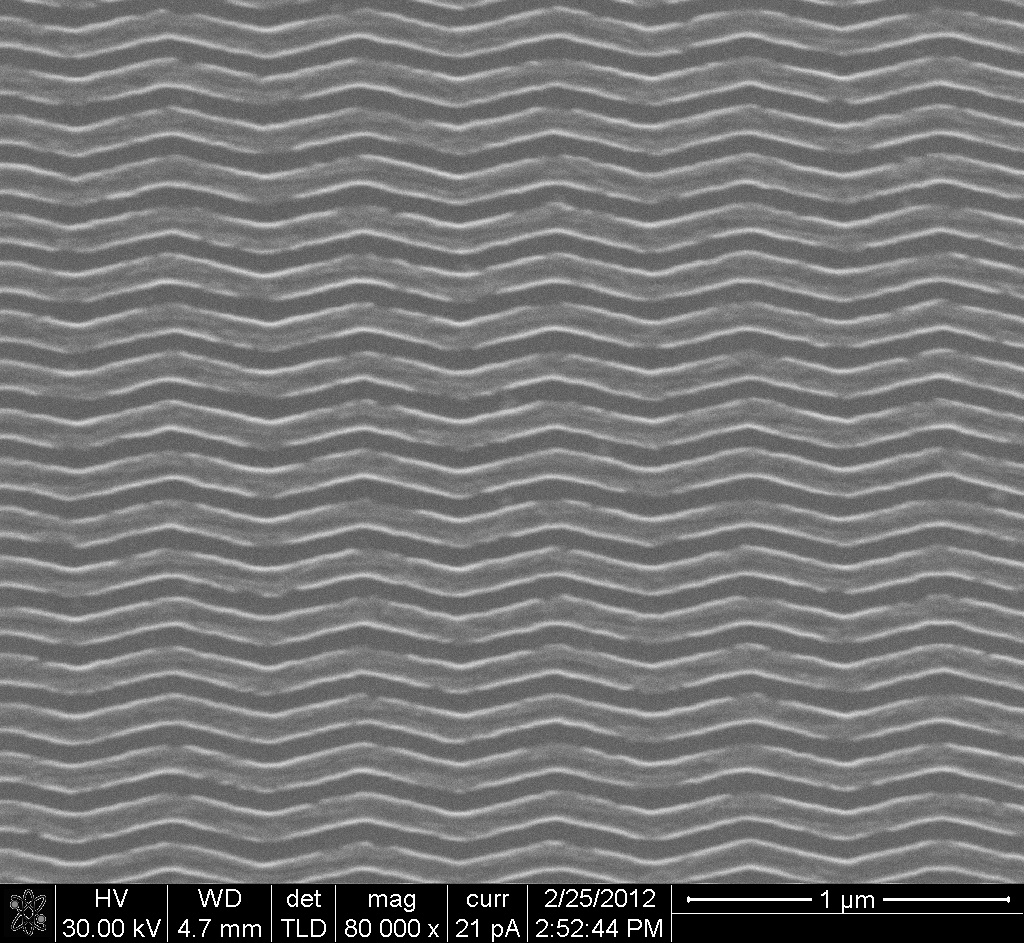
\includegraphics[width=0.32\linewidth]{sems/RIE_area1_008.jpg}\label{fig:sem-master}}
\subfigure[]{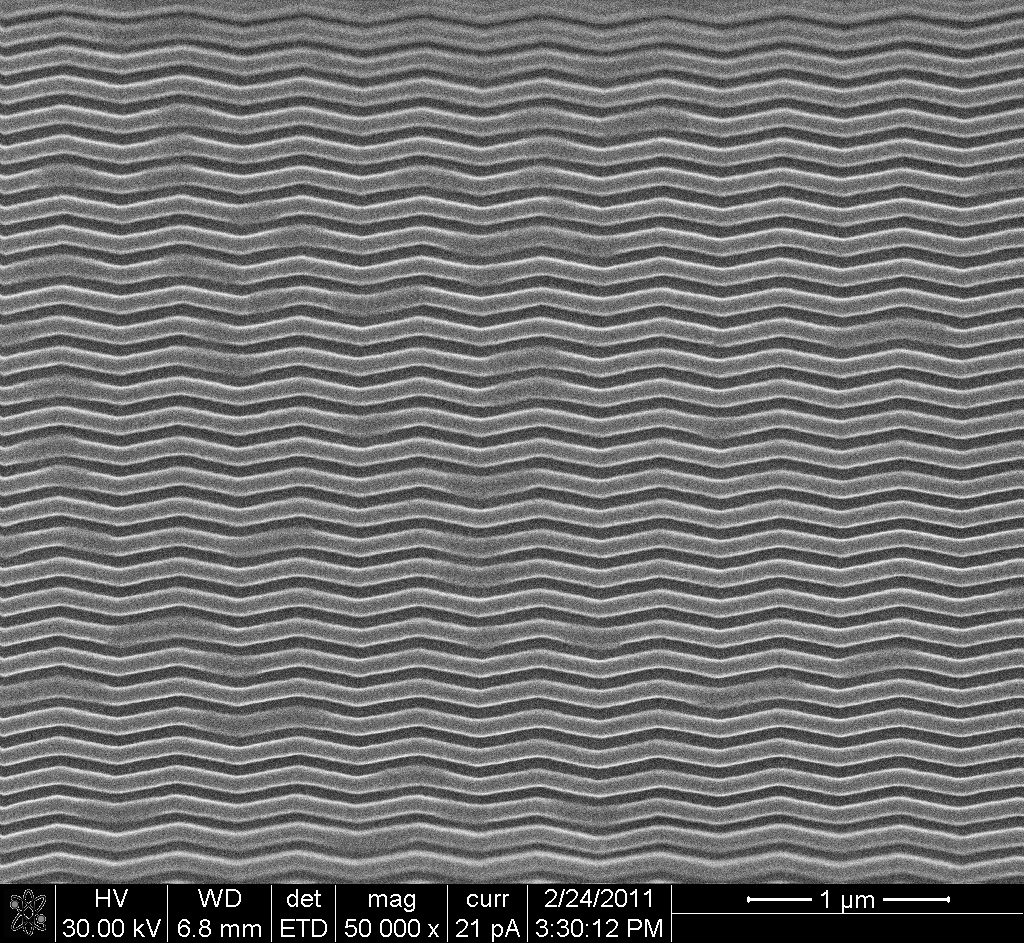
\includegraphics[width=0.32\linewidth]{sems/zigzag1_003.jpg}\label{fig:sem-polymer}}
\subfigure[]{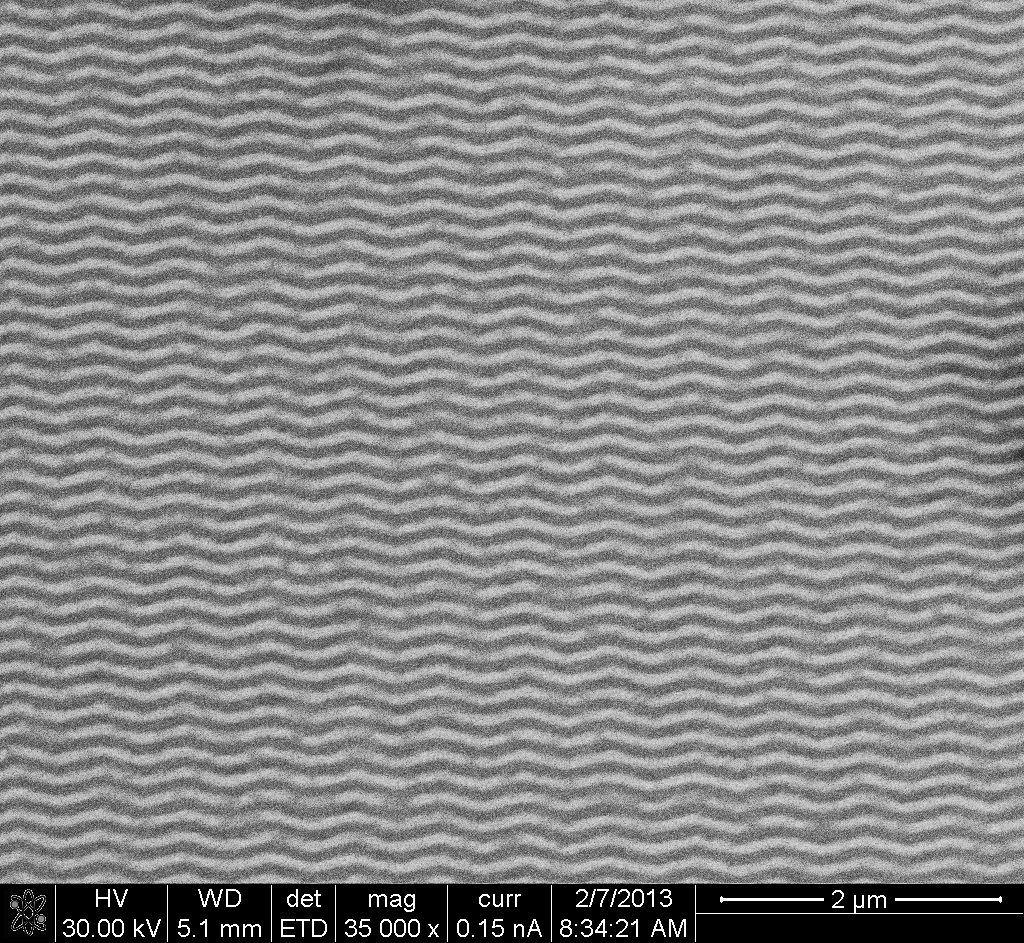
\includegraphics[width=0.32\linewidth]{pic_003}\label{fig:sem-ts}}
\end{center}
\caption[Scanning electron micrographs of various zigzag grating samples.]{Scanning electron micrographs of: (a) an example template-strip master in Si, used for production of zigzag gratings; (b) a polymer replica of a Si master prior to metallisation, for zigzag gratings embedded in glass; (c) a template stripped sample in silver.}
\end{figure}

Results from two different versions of this zigzag grating sample are presented in this chapter. One is a zigzag grating produced by the template stripping method detailed in chapter \ref{c:experimentalmethods}, the SPPs propagating along the air/metal interface. The second sample is the same zigzag grating embedded in glass, so that the SPPs propagate along the glass/metal interface. The reason for the two samples is that observation of novel higher-frequency modes, such as the $3^{rd}$ order diffracted SPPs, may be out of the visible domain when the SPP propagates along the air/metal interface. Using a higher index bounding material, the phase velocity of the SPPs is reduced and so for the same value of in-plane momentum, these modes may be brought down in frequency into the visible domain. The glass/grating sample was produced using a slightly different embossing method, detailed below. In each section, the grating used is clearly stated at the start.

For the glass/grating sample, the structure was duplicated in UV-cured polymer. Scanning electron microscopy was used to image the surface of this zigzag grating  replica in the polymer (figure \ref{fig:sem-polymer}), prior to metallisation. From this micrograph, the mark-to-space ratio of the final grating structure was determined to be 0.75 with ${\lambda_{gx} = 600 \pm 5 \:\nano\metre}$, and ${\lambda_{gy} = 150 \pm 5 \nano\metre}$. This pattern was then transferred to another UV cured polymer (Norland Optical Adhesive 73) adhered to a glass substrate (${n_{632.8 \:\nano\metre} = 1.518}$) using an embossing method.
Silver was thermally evaporated under high vacuum ($5 \times 10^{-6}$ mbar) with ${50 \:\nano\metre}$ depositions followed by 10 minutes relaxation time repeated until an optically thick layer of ${200\:\nano\metre}$ was recorded on the quartz crystal thickness monitor. This stepped procedure was used to prevent the temperature rising on the substrate enough to damage the polymer.
The substrate was then adhered to the back of a prepared glass hemisphere of radius 21.75 mm and refractive index $n$ = 1.518 using index matching fluid, the base of the hemisphere having been modified by removing ${1 \:\milli\metre}$ to account for the affixed substrate thickness. This arrangement allows illumination of the embedded grating structure at the metal/glass interface at all angles of incidence. The mounting also protects the surface of the silver from sulphur contamination \cite{Kovacs1978}.

\subsection{Transverse Electric Coupling\label{sec:TEexciatation}}

The dispersion of the SPPs supported on a zigzag grating is mapped as a function of in plane wavevector, $\mathbf{k}_{gx}$, by varying the polar angle $\theta$ and angular frequency, $\omega$, using a polarised, collimated, monochromatic beam, produced by a white light source together with a spectrometer. The wavelength range used was $400 < \lambda_0 < 850$ nm with the angle range $7^\circ<\theta<60^\circ$ (see chapter \ref{c:experimentalmethods}). When the energy and in-plane momentum of the light matches that of a SPP mode, the light couples to a SPP and an extremum of the reflectivity is observed. The experimental and theoretical reflectivity of incident TE polarised light at $\phi = 0^\circ$ is shown in figure \ref{fig:TEdiseprsionInAir}, for a zigzag grating in air. 

\begin{figure}
	\begin{center}
		\subfigure[]{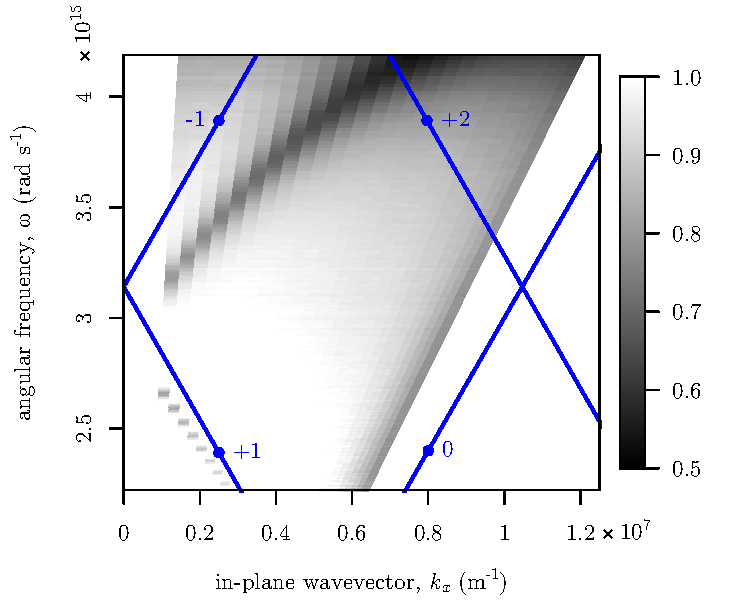
\includegraphics[width=0.49\linewidth]{dispersionplots-air/figure-zigzag-air-disperison-experiement-rss.pdf}\label{fig:TEdiseprsionInAira}}
		\subfigure[]{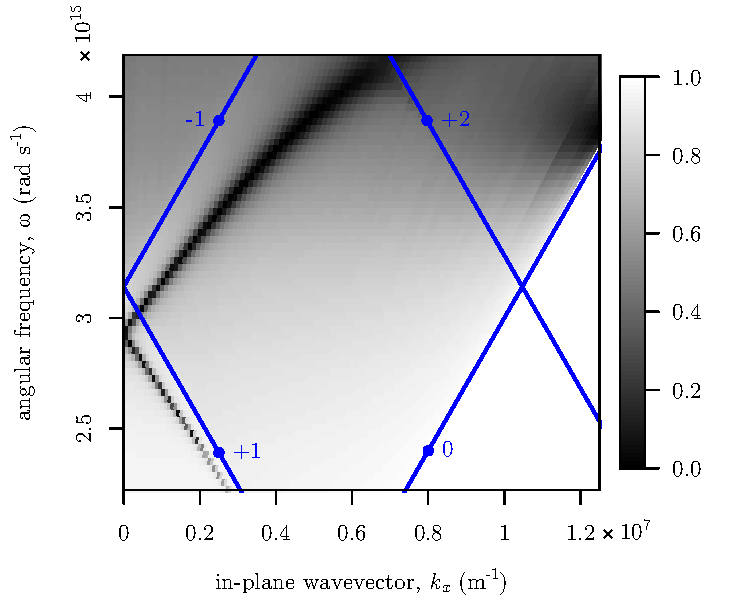
\includegraphics[width=0.49\linewidth]{dispersionplots-air/figure-zigzag-air-disperison-theory-rss.pdf}\label{fig:TEdiseprsionInAirb}} 
	\end{center}
	
	\caption[SPP dispersion on a zigzag grating measured using TE polarised light.]{Experimental data (a) and FEM model prediction (b) of TE polarised reflectivity as a function of in-plane wavevector and angular frequency, mapping  SPP dispersion on a zigzag grating. \color{blue}Blue \color{black} lines show the positions of diffracted light lines scattered by $m\mathbf{k}_{gx}$, where $m = \pm 1, +2,  0$\label{fig:TEdiseprsionInAir}}
\end{figure}

Two dark bands of low reflectivity are observed associated with the $\pm\mathbf{k}_{gx}$ light lines (blue lines). These bands map the position in $\omega-k_x$ space of SPPs scattered by grating vectors equal to  $\mathbf{k}_{SPP}=\mathbf{k}_x\pm \mathbf{k}_{gx}$. As predicted by equation \ref{eq:zz-tecoupling}, this odd-scattered mode is coupled to by TE polarised light. The dispersion of the mode in the experimental data (figure \ref{fig:TEdiseprsionInAira}) and theoretical model obtained using FEM (figure \ref{fig:TEdiseprsionInAirb}) show excellent agreement. The model parameters used were for a depth of 70 nm and a mark-to-space ratio between the sub-wavelength grooves of 1, using the silver dielectric function as reported by Nash \& Sambles \cite{Nash1996}. The experimental sample is expected to be shallower than the designed 70 nm from duplication, leading to the observation that the experimental SPP is not coupled optimally to the incident light, and so the reflectivity band is not as dark as the FEM prediction.

This band of low reflectivity is investigated further in figure \ref{fig:anglescan}. The reflected intensity of light from a zigzag grating embedded in glass is illuminated with TE polarised light, at a wavelength of 632.8 nm, and recorded as a function of the polar angle of incidence, $\theta$. 
\begin{figure}
\begin{center}
% Created by tikzDevice version 0.6.2-92-0ad2792 on 2012-10-09 17:04:50
% !TEX encoding = UTF-8 Unicode
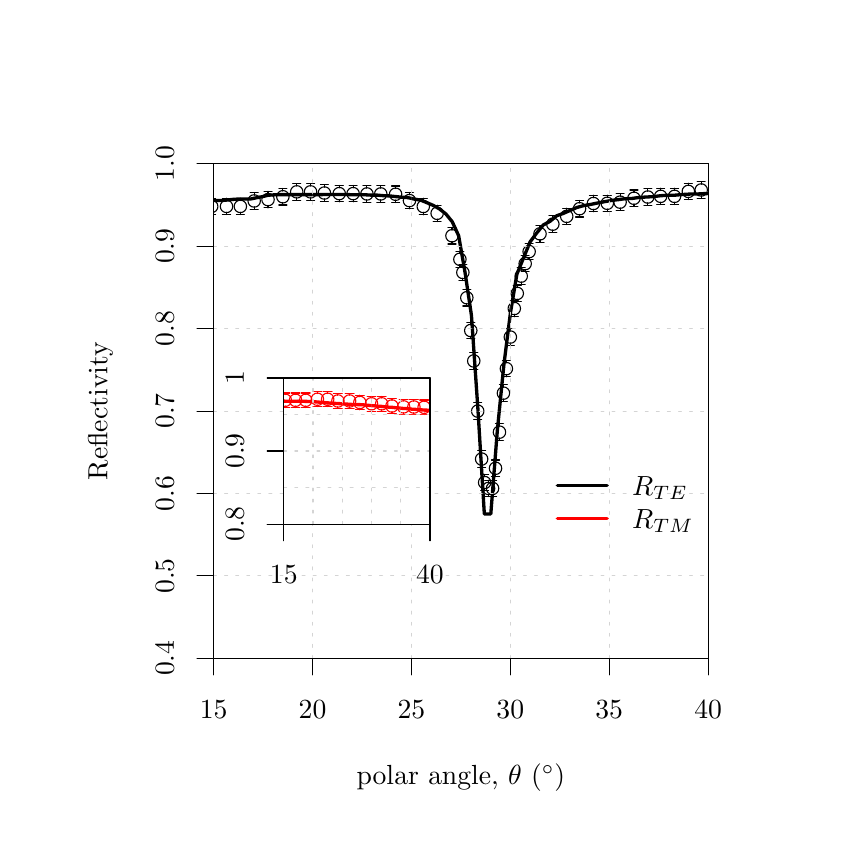
\begin{tikzpicture}[x=1pt,y=1pt]
\definecolor[named]{fillColor}{rgb}{1.00,1.00,1.00}
\path[use as bounding box,fill=fillColor,fill opacity=0.00] (0,0) rectangle (289.08,289.08);
\begin{scope}
\path[clip] ( 67.20, 61.20) rectangle (245.88,239.88);
\definecolor[named]{drawColor}{rgb}{0.00,0.00,0.00}

\path[draw=drawColor,line width= 1.2pt,line join=round,line cap=round] (  1.01,225.70) --
	(  3.07,225.70) --
	(  5.13,225.70) --
	(  7.19,225.70) --
	(  9.25,225.73) --
	( 11.31,225.73) --
	( 13.38,225.73) --
	( 15.44,225.73) --
	( 17.51,225.73) --
	( 19.58,225.78) --
	( 21.65,225.78) --
	( 23.72,225.78) --
	( 25.80,225.78) --
	( 27.87,225.78) --
	( 29.95,225.84) --
	( 32.03,225.88) --
	( 34.11,225.88) --
	( 36.19,225.88) --
	( 38.27,225.88) --
	( 40.36,225.78) --
	( 42.45,225.78) --
	( 44.54,225.78) --
	( 46.63,225.95) --
	( 48.73,225.99) --
	( 50.83,226.22) --
	( 52.93,226.22) --
	( 55.03,226.22) --
	( 57.13,226.32) --
	( 59.24,226.32) --
	( 61.35,226.32) --
	( 63.47,226.47) --
	( 65.58,226.60) --
	( 67.70,226.60) --
	( 69.82,226.60) --
	( 71.95,226.78) --
	( 74.08,227.02) --
	( 76.21,227.16) --
	( 78.34,227.16) --
	( 80.48,227.16) --
	( 82.62,227.61) --
	( 84.76,228.01) --
	( 86.91,228.53) --
	( 89.06,228.67) --
	( 91.22,228.75) --
	( 93.38,228.75) --
	( 95.54,228.75) --
	( 97.71,228.75) --
	( 99.88,228.75) --
	(102.06,228.75) --
	(104.24,228.75) --
	(106.42,228.76) --
	(108.61,228.78) --
	(110.80,228.78) --
	(113.00,228.78) --
	(115.20,228.78) --
	(117.40,228.70) --
	(119.62,228.70) --
	(121.83,228.70) --
	(124.05,228.57) --
	(126.28,228.57) --
	(128.51,228.37) --
	(130.75,228.28) --
	(132.99,228.04) --
	(135.24,227.81) --
	(137.49,227.65) --
	(139.75,227.12) --
	(142.01,226.75) --
	(144.28,225.83) --
	(146.56,224.86) --
	(148.84,223.55) --
	(151.13,221.76) --
	(153.43,218.93) --
	(155.73,213.89) --
	(158.04,200.66) --
	(160.36,185.07) --
	(162.68,151.45) --
	(165.01,113.36) --
	(167.35,113.36) --
	(169.70,143.43) --
	(172.05,167.01) --
	(174.41,185.80) --
	(176.78,200.01) --
	(179.15,205.83) --
	(181.54,211.66) --
	(183.93,214.87) --
	(186.33,217.80) --
	(188.74,219.09) --
	(191.16,221.10) --
	(193.59,221.98) --
	(198.47,224.11) --
	(200.93,224.79) --
	(203.40,225.20) --
	(205.87,225.71) --
	(208.36,226.18) --
	(210.86,226.64) --
	(213.36,226.93) --
	(215.88,227.27) --
	(218.41,227.37) --
	(220.96,227.73) --
	(223.51,227.88) --
	(226.07,228.02) --
	(228.65,228.35) --
	(231.24,228.53) --
	(233.85,228.54) --
	(236.46,228.78) --
	(239.09,228.94) --
	(241.73,228.97) --
	(244.39,229.11) --
	(247.06,229.14) --
	(249.75,229.40) --
	(252.45,229.45) --
	(255.17,229.48) --
	(257.90,229.64) --
	(260.65,229.72) --
	(263.42,229.84) --
	(266.20,229.95) --
	(269.01,230.01) --
	(271.83,230.01) --
	(274.66,230.01) --
	(277.52,230.32) --
	(280.40,230.38) --
	(283.29,230.38) --
	(286.21,230.56) --
	(289.08,230.67);
\end{scope}
\begin{scope}
\path[clip] (  0.00,  0.00) rectangle (289.08,289.08);
\definecolor[named]{drawColor}{rgb}{0.00,0.00,0.00}
\definecolor[named]{fillColor}{rgb}{1.00,1.00,1.00}

\path[draw=drawColor,line width= 0.4pt,line join=round,line cap=round,fill=fillColor] ( 67.20, 61.20) -- (245.88, 61.20);

\path[draw=drawColor,line width= 0.4pt,line join=round,line cap=round,fill=fillColor] ( 67.20, 61.20) -- ( 67.20, 55.20);

\path[draw=drawColor,line width= 0.4pt,line join=round,line cap=round,fill=fillColor] (102.94, 61.20) -- (102.94, 55.20);

\path[draw=drawColor,line width= 0.4pt,line join=round,line cap=round,fill=fillColor] (138.67, 61.20) -- (138.67, 55.20);

\path[draw=drawColor,line width= 0.4pt,line join=round,line cap=round,fill=fillColor] (174.41, 61.20) -- (174.41, 55.20);

\path[draw=drawColor,line width= 0.4pt,line join=round,line cap=round,fill=fillColor] (210.14, 61.20) -- (210.14, 55.20);

\path[draw=drawColor,line width= 0.4pt,line join=round,line cap=round,fill=fillColor] (245.88, 61.20) -- (245.88, 55.20);

\node[text=drawColor,anchor=base,inner sep=0pt, outer sep=0pt, scale=  1.00] at ( 67.20, 39.60) {15};

\node[text=drawColor,anchor=base,inner sep=0pt, outer sep=0pt, scale=  1.00] at (102.94, 39.60) {20};

\node[text=drawColor,anchor=base,inner sep=0pt, outer sep=0pt, scale=  1.00] at (138.67, 39.60) {25};

\node[text=drawColor,anchor=base,inner sep=0pt, outer sep=0pt, scale=  1.00] at (174.41, 39.60) {30};

\node[text=drawColor,anchor=base,inner sep=0pt, outer sep=0pt, scale=  1.00] at (210.14, 39.60) {35};

\node[text=drawColor,anchor=base,inner sep=0pt, outer sep=0pt, scale=  1.00] at (245.88, 39.60) {40};

\path[draw=drawColor,line width= 0.4pt,line join=round,line cap=round,fill=fillColor] ( 67.20, 61.20) -- ( 67.20,239.88);

\path[draw=drawColor,line width= 0.4pt,line join=round,line cap=round,fill=fillColor] ( 67.20, 61.20) -- ( 61.20, 61.20);

\path[draw=drawColor,line width= 0.4pt,line join=round,line cap=round,fill=fillColor] ( 67.20, 90.98) -- ( 61.20, 90.98);

\path[draw=drawColor,line width= 0.4pt,line join=round,line cap=round,fill=fillColor] ( 67.20,120.76) -- ( 61.20,120.76);

\path[draw=drawColor,line width= 0.4pt,line join=round,line cap=round,fill=fillColor] ( 67.20,150.54) -- ( 61.20,150.54);

\path[draw=drawColor,line width= 0.4pt,line join=round,line cap=round,fill=fillColor] ( 67.20,180.32) -- ( 61.20,180.32);

\path[draw=drawColor,line width= 0.4pt,line join=round,line cap=round,fill=fillColor] ( 67.20,210.10) -- ( 61.20,210.10);

\path[draw=drawColor,line width= 0.4pt,line join=round,line cap=round,fill=fillColor] ( 67.20,239.88) -- ( 61.20,239.88);

\node[text=drawColor,rotate= 90.00,anchor=base,inner sep=0pt, outer sep=0pt, scale=  1.00] at ( 52.80, 61.20) {0.4};

\node[text=drawColor,rotate= 90.00,anchor=base,inner sep=0pt, outer sep=0pt, scale=  1.00] at ( 52.80, 90.98) {0.5};

\node[text=drawColor,rotate= 90.00,anchor=base,inner sep=0pt, outer sep=0pt, scale=  1.00] at ( 52.80,120.76) {0.6};

\node[text=drawColor,rotate= 90.00,anchor=base,inner sep=0pt, outer sep=0pt, scale=  1.00] at ( 52.80,150.54) {0.7};

\node[text=drawColor,rotate= 90.00,anchor=base,inner sep=0pt, outer sep=0pt, scale=  1.00] at ( 52.80,180.32) {0.8};

\node[text=drawColor,rotate= 90.00,anchor=base,inner sep=0pt, outer sep=0pt, scale=  1.00] at ( 52.80,210.10) {0.9};

\node[text=drawColor,rotate= 90.00,anchor=base,inner sep=0pt, outer sep=0pt, scale=  1.00] at ( 52.80,239.88) {1.0};

\path[draw=drawColor,line width= 0.4pt,line join=round,line cap=round] ( 67.20, 61.20) --
	(245.88, 61.20) --
	(245.88,239.88) --
	( 67.20,239.88) --
	( 67.20, 61.20);
\end{scope}
\begin{scope}
\path[clip] (  0.00,  0.00) rectangle (289.08,289.08);
\definecolor[named]{drawColor}{rgb}{0.00,0.00,0.00}

\node[text=drawColor,anchor=base,inner sep=0pt, outer sep=0pt, scale=  1.00] at (156.54, 15.60) {polar angle, $\theta$ ($^{\circ}$)};

\node[text=drawColor,rotate= 90.00,anchor=base,inner sep=0pt, outer sep=0pt, scale=  1.00] at ( 28.80,150.54) {Reflectivity};
\end{scope}
\begin{scope}
\path[clip] ( 67.20, 61.20) rectangle (245.88,239.88);
\definecolor[named]{drawColor}{rgb}{0.00,0.00,0.00}
\definecolor[named]{fillColor}{rgb}{1.00,1.00,1.00}

\path[draw=drawColor,line width= 0.4pt,line join=round,line cap=round,fill=fillColor] ( 36.11,221.75) -- ( 36.11,222.66);

\path[draw=drawColor,line width= 0.4pt,line join=round,line cap=round] ( 34.66,221.75) --
	( 36.11,221.75) --
	( 37.56,221.75);

\path[draw=drawColor,line width= 0.4pt,line join=round,line cap=round,fill=fillColor] ( 41.11,221.75) -- ( 41.11,222.66);

\path[draw=drawColor,line width= 0.4pt,line join=round,line cap=round] ( 39.67,221.75) --
	( 41.11,221.75) --
	( 42.56,221.75);

\path[draw=drawColor,line width= 0.4pt,line join=round,line cap=round,fill=fillColor] ( 46.12,221.90) -- ( 46.12,222.81);

\path[draw=drawColor,line width= 0.4pt,line join=round,line cap=round] ( 44.67,221.90) --
	( 46.12,221.90) --
	( 47.56,221.90);

\path[draw=drawColor,line width= 0.4pt,line join=round,line cap=round,fill=fillColor] ( 51.48,222.20) -- ( 51.48,223.11);

\path[draw=drawColor,line width= 0.4pt,line join=round,line cap=round] ( 50.03,222.20) --
	( 51.48,222.20) --
	( 52.92,222.20);

\path[draw=drawColor,line width= 0.4pt,line join=round,line cap=round,fill=fillColor] ( 56.48,222.20) -- ( 56.48,223.11);

\path[draw=drawColor,line width= 0.4pt,line join=round,line cap=round] ( 55.03,222.20) --
	( 56.48,222.20) --
	( 57.92,222.20);

\path[draw=drawColor,line width= 0.4pt,line join=round,line cap=round,fill=fillColor] ( 61.48,221.95) -- ( 61.48,222.86);

\path[draw=drawColor,line width= 0.4pt,line join=round,line cap=round] ( 60.04,221.95) --
	( 61.48,221.95) --
	( 62.93,221.95);

\path[draw=drawColor,line width= 0.4pt,line join=round,line cap=round,fill=fillColor] ( 66.49,221.51) -- ( 66.49,222.43);

\path[draw=drawColor,line width= 0.4pt,line join=round,line cap=round] ( 65.04,221.51) --
	( 66.49,221.51) --
	( 67.93,221.51);

\path[draw=drawColor,line width= 0.4pt,line join=round,line cap=round,fill=fillColor] ( 71.85,221.51) -- ( 71.85,222.43);

\path[draw=drawColor,line width= 0.4pt,line join=round,line cap=round] ( 70.40,221.51) --
	( 71.85,221.51) --
	( 73.29,221.51);

\path[draw=drawColor,line width= 0.4pt,line join=round,line cap=round,fill=fillColor] ( 76.85,221.51) -- ( 76.85,222.43);

\path[draw=drawColor,line width= 0.4pt,line join=round,line cap=round] ( 75.40,221.51) --
	( 76.85,221.51) --
	( 78.29,221.51);

\path[draw=drawColor,line width= 0.4pt,line join=round,line cap=round,fill=fillColor] ( 81.85,223.48) -- ( 81.85,224.39);

\path[draw=drawColor,line width= 0.4pt,line join=round,line cap=round] ( 80.41,223.48) --
	( 81.85,223.48) --
	( 83.30,223.48);

\path[draw=drawColor,line width= 0.4pt,line join=round,line cap=round,fill=fillColor] ( 86.85,223.97) -- ( 86.85,224.88);

\path[draw=drawColor,line width= 0.4pt,line join=round,line cap=round] ( 85.41,223.97) --
	( 86.85,223.97) --
	( 88.30,223.97);

\path[draw=drawColor,line width= 0.4pt,line join=round,line cap=round,fill=fillColor] ( 92.22,225.00) -- ( 92.22,225.91);

\path[draw=drawColor,line width= 0.4pt,line join=round,line cap=round] ( 90.77,225.00) --
	( 92.22,225.00) --
	( 93.66,225.00);

\path[draw=drawColor,line width= 0.4pt,line join=round,line cap=round,fill=fillColor] ( 97.22,226.78) -- ( 97.22,227.69);

\path[draw=drawColor,line width= 0.4pt,line join=round,line cap=round] ( 95.77,226.78) --
	( 97.22,226.78) --
	( 98.66,226.78);

\path[draw=drawColor,line width= 0.4pt,line join=round,line cap=round,fill=fillColor] (102.22,226.78) -- (102.22,227.69);

\path[draw=drawColor,line width= 0.4pt,line join=round,line cap=round] (100.78,226.78) --
	(102.22,226.78) --
	(103.67,226.78);

\path[draw=drawColor,line width= 0.4pt,line join=round,line cap=round,fill=fillColor] (107.22,226.35) -- (107.22,227.26);

\path[draw=drawColor,line width= 0.4pt,line join=round,line cap=round] (105.78,226.35) --
	(107.22,226.35) --
	(108.67,226.35);

\path[draw=drawColor,line width= 0.4pt,line join=round,line cap=round,fill=fillColor] (112.58,226.13) -- (112.58,227.05);

\path[draw=drawColor,line width= 0.4pt,line join=round,line cap=round] (111.14,226.13) --
	(112.58,226.13) --
	(114.03,226.13);

\path[draw=drawColor,line width= 0.4pt,line join=round,line cap=round,fill=fillColor] (117.59,226.13) -- (117.59,227.05);

\path[draw=drawColor,line width= 0.4pt,line join=round,line cap=round] (116.14,226.13) --
	(117.59,226.13) --
	(119.03,226.13);

\path[draw=drawColor,line width= 0.4pt,line join=round,line cap=round,fill=fillColor] (122.59,226.02) -- (122.59,226.93);

\path[draw=drawColor,line width= 0.4pt,line join=round,line cap=round] (121.15,226.02) --
	(122.59,226.02) --
	(124.04,226.02);

\path[draw=drawColor,line width= 0.4pt,line join=round,line cap=round,fill=fillColor] (127.59,226.02) -- (127.59,226.93);

\path[draw=drawColor,line width= 0.4pt,line join=round,line cap=round] (126.15,226.02) --
	(127.59,226.02) --
	(129.04,226.02);

\path[draw=drawColor,line width= 0.4pt,line join=round,line cap=round,fill=fillColor] (132.95,225.91) -- (132.95,226.82);

\path[draw=drawColor,line width= 0.4pt,line join=round,line cap=round] (131.51,225.91) --
	(132.95,225.91) --
	(134.40,225.91);

\path[draw=drawColor,line width= 0.4pt,line join=round,line cap=round,fill=fillColor] (137.96,223.62) -- (137.96,224.53);

\path[draw=drawColor,line width= 0.4pt,line join=round,line cap=round] (136.51,223.62) --
	(137.96,223.62) --
	(139.40,223.62);

\path[draw=drawColor,line width= 0.4pt,line join=round,line cap=round,fill=fillColor] (142.96,221.48) -- (142.96,222.39);

\path[draw=drawColor,line width= 0.4pt,line join=round,line cap=round] (141.51,221.48) --
	(142.96,221.48) --
	(144.41,221.48);

\path[draw=drawColor,line width= 0.4pt,line join=round,line cap=round,fill=fillColor] (147.96,219.02) -- (147.96,219.93);

\path[draw=drawColor,line width= 0.4pt,line join=round,line cap=round] (146.52,219.02) --
	(147.96,219.02) --
	(149.41,219.02);

\path[draw=drawColor,line width= 0.4pt,line join=round,line cap=round,fill=fillColor] (153.32,210.90) -- (153.32,211.81);

\path[draw=drawColor,line width= 0.4pt,line join=round,line cap=round] (151.88,210.90) --
	(153.32,210.90) --
	(154.77,210.90);

\path[draw=drawColor,line width= 0.4pt,line join=round,line cap=round,fill=fillColor] (156.18,202.40) -- (156.18,203.31);

\path[draw=drawColor,line width= 0.4pt,line join=round,line cap=round] (154.74,202.40) --
	(156.18,202.40) --
	(157.63,202.40);

\path[draw=drawColor,line width= 0.4pt,line join=round,line cap=round,fill=fillColor] (157.25,197.65) -- (157.25,198.56);

\path[draw=drawColor,line width= 0.4pt,line join=round,line cap=round] (155.81,197.65) --
	(157.25,197.65) --
	(158.70,197.65);

\path[draw=drawColor,line width= 0.4pt,line join=round,line cap=round,fill=fillColor] (158.68,188.51) -- (158.68,189.42);

\path[draw=drawColor,line width= 0.4pt,line join=round,line cap=round] (157.24,188.51) --
	(158.68,188.51) --
	(160.13,188.51);

\path[draw=drawColor,line width= 0.4pt,line join=round,line cap=round,fill=fillColor] (160.11,176.66) -- (160.11,177.57);

\path[draw=drawColor,line width= 0.4pt,line join=round,line cap=round] (158.67,176.66) --
	(160.11,176.66) --
	(161.56,176.66);

\path[draw=drawColor,line width= 0.4pt,line join=round,line cap=round,fill=fillColor] (161.19,165.67) -- (161.19,166.58);

\path[draw=drawColor,line width= 0.4pt,line join=round,line cap=round] (159.74,165.67) --
	(161.19,165.67) --
	(162.63,165.67);

\path[draw=drawColor,line width= 0.4pt,line join=round,line cap=round,fill=fillColor] (162.62,147.54) -- (162.62,148.45);

\path[draw=drawColor,line width= 0.4pt,line join=round,line cap=round] (161.17,147.54) --
	(162.62,147.54) --
	(164.06,147.54);

\path[draw=drawColor,line width= 0.4pt,line join=round,line cap=round,fill=fillColor] (164.04,130.22) -- (164.04,131.14);

\path[draw=drawColor,line width= 0.4pt,line join=round,line cap=round] (162.60,130.22) --
	(164.04,130.22) --
	(165.49,130.22);

\path[draw=drawColor,line width= 0.4pt,line join=round,line cap=round,fill=fillColor] (165.12,121.73) -- (165.12,122.64);

\path[draw=drawColor,line width= 0.4pt,line join=round,line cap=round] (163.67,121.73) --
	(165.12,121.73) --
	(166.56,121.73);

\path[draw=drawColor,line width= 0.4pt,line join=round,line cap=round,fill=fillColor] (166.55,119.62) -- (166.55,120.53);

\path[draw=drawColor,line width= 0.4pt,line join=round,line cap=round] (165.10,119.62) --
	(166.55,119.62) --
	(167.99,119.62);

\path[draw=drawColor,line width= 0.4pt,line join=round,line cap=round,fill=fillColor] (167.98,119.62) -- (167.98,120.53);

\path[draw=drawColor,line width= 0.4pt,line join=round,line cap=round] (166.53,119.62) --
	(167.98,119.62) --
	(169.42,119.62);

\path[draw=drawColor,line width= 0.4pt,line join=round,line cap=round,fill=fillColor] (169.05,126.89) -- (169.05,127.80);

\path[draw=drawColor,line width= 0.4pt,line join=round,line cap=round] (167.60,126.89) --
	(169.05,126.89) --
	(170.49,126.89);

\path[draw=drawColor,line width= 0.4pt,line join=round,line cap=round,fill=fillColor] (170.48,139.94) -- (170.48,140.85);

\path[draw=drawColor,line width= 0.4pt,line join=round,line cap=round] (169.03,139.94) --
	(170.48,139.94) --
	(171.92,139.94);

\path[draw=drawColor,line width= 0.4pt,line join=round,line cap=round,fill=fillColor] (171.91,154.05) -- (171.91,154.96);

\path[draw=drawColor,line width= 0.4pt,line join=round,line cap=round] (170.46,154.05) --
	(171.91,154.05) --
	(173.35,154.05);

\path[draw=drawColor,line width= 0.4pt,line join=round,line cap=round,fill=fillColor] (172.98,162.89) -- (172.98,163.80);

\path[draw=drawColor,line width= 0.4pt,line join=round,line cap=round] (171.53,162.89) --
	(172.98,162.89) --
	(174.42,162.89);

\path[draw=drawColor,line width= 0.4pt,line join=round,line cap=round,fill=fillColor] (174.41,174.30) -- (174.41,175.21);

\path[draw=drawColor,line width= 0.4pt,line join=round,line cap=round] (172.96,174.30) --
	(174.41,174.30) --
	(175.85,174.30);

\path[draw=drawColor,line width= 0.4pt,line join=round,line cap=round,fill=fillColor] (175.84,184.63) -- (175.84,185.54);

\path[draw=drawColor,line width= 0.4pt,line join=round,line cap=round] (174.39,184.63) --
	(175.84,184.63) --
	(177.28,184.63);

\path[draw=drawColor,line width= 0.4pt,line join=round,line cap=round,fill=fillColor] (176.91,190.08) -- (176.91,190.99);

\path[draw=drawColor,line width= 0.4pt,line join=round,line cap=round] (175.46,190.08) --
	(176.91,190.08) --
	(178.35,190.08);

\path[draw=drawColor,line width= 0.4pt,line join=round,line cap=round,fill=fillColor] (178.34,196.32) -- (178.34,197.23);

\path[draw=drawColor,line width= 0.4pt,line join=round,line cap=round] (176.89,196.32) --
	(178.34,196.32) --
	(179.78,196.32);

\path[draw=drawColor,line width= 0.4pt,line join=round,line cap=round,fill=fillColor] (179.77,200.83) -- (179.77,201.74);

\path[draw=drawColor,line width= 0.4pt,line join=round,line cap=round] (178.32,200.83) --
	(179.77,200.83) --
	(181.21,200.83);

\path[draw=drawColor,line width= 0.4pt,line join=round,line cap=round,fill=fillColor] (181.20,205.19) -- (181.20,206.10);

\path[draw=drawColor,line width= 0.4pt,line join=round,line cap=round] (179.75,205.19) --
	(181.20,205.19) --
	(182.64,205.19);

\path[draw=drawColor,line width= 0.4pt,line join=round,line cap=round,fill=fillColor] (185.13,211.60) -- (185.13,212.51);

\path[draw=drawColor,line width= 0.4pt,line join=round,line cap=round] (183.68,211.60) --
	(185.13,211.60) --
	(186.57,211.60);

\path[draw=drawColor,line width= 0.4pt,line join=round,line cap=round,fill=fillColor] (189.77,215.10) -- (189.77,216.01);

\path[draw=drawColor,line width= 0.4pt,line join=round,line cap=round] (188.33,215.10) --
	(189.77,215.10) --
	(191.22,215.10);

\path[draw=drawColor,line width= 0.4pt,line join=round,line cap=round,fill=fillColor] (194.78,217.93) -- (194.78,218.84);

\path[draw=drawColor,line width= 0.4pt,line join=round,line cap=round] (193.33,217.93) --
	(194.78,217.93) --
	(196.22,217.93);

\path[draw=drawColor,line width= 0.4pt,line join=round,line cap=round,fill=fillColor] (199.42,220.68) -- (199.42,221.59);

\path[draw=drawColor,line width= 0.4pt,line join=round,line cap=round] (197.98,220.68) --
	(199.42,220.68) --
	(200.87,220.68);

\path[draw=drawColor,line width= 0.4pt,line join=round,line cap=round,fill=fillColor] (204.43,222.57) -- (204.43,223.48);

\path[draw=drawColor,line width= 0.4pt,line join=round,line cap=round] (202.98,222.57) --
	(204.43,222.57) --
	(205.87,222.57);

\path[draw=drawColor,line width= 0.4pt,line join=round,line cap=round,fill=fillColor] (209.43,222.64) -- (209.43,223.55);

\path[draw=drawColor,line width= 0.4pt,line join=round,line cap=round] (207.98,222.64) --
	(209.43,222.64) --
	(210.87,222.64);

\path[draw=drawColor,line width= 0.4pt,line join=round,line cap=round,fill=fillColor] (214.07,223.05) -- (214.07,223.96);

\path[draw=drawColor,line width= 0.4pt,line join=round,line cap=round] (212.63,223.05) --
	(214.07,223.05) --
	(215.52,223.05);

\path[draw=drawColor,line width= 0.4pt,line join=round,line cap=round,fill=fillColor] (219.08,224.46) -- (219.08,225.37);

\path[draw=drawColor,line width= 0.4pt,line join=round,line cap=round] (217.63,224.46) --
	(219.08,224.46) --
	(220.52,224.46);

\path[draw=drawColor,line width= 0.4pt,line join=round,line cap=round,fill=fillColor] (224.08,224.90) -- (224.08,225.81);

\path[draw=drawColor,line width= 0.4pt,line join=round,line cap=round] (222.64,224.90) --
	(224.08,224.90) --
	(225.53,224.90);

\path[draw=drawColor,line width= 0.4pt,line join=round,line cap=round,fill=fillColor] (228.73,225.15) -- (228.73,226.06);

\path[draw=drawColor,line width= 0.4pt,line join=round,line cap=round] (227.28,225.15) --
	(228.73,225.15) --
	(230.17,225.15);

\path[draw=drawColor,line width= 0.4pt,line join=round,line cap=round,fill=fillColor] (233.73,225.15) -- (233.73,226.06);

\path[draw=drawColor,line width= 0.4pt,line join=round,line cap=round] (232.28,225.15) --
	(233.73,225.15) --
	(235.18,225.15);

\path[draw=drawColor,line width= 0.4pt,line join=round,line cap=round,fill=fillColor] (238.73,226.94) -- (238.73,227.86);

\path[draw=drawColor,line width= 0.4pt,line join=round,line cap=round] (237.29,226.94) --
	(238.73,226.94) --
	(240.18,226.94);

\path[draw=drawColor,line width= 0.4pt,line join=round,line cap=round,fill=fillColor] (243.38,227.45) -- (243.38,228.36);

\path[draw=drawColor,line width= 0.4pt,line join=round,line cap=round] (241.93,227.45) --
	(243.38,227.45) --
	(244.82,227.45);

\path[draw=drawColor,line width= 0.4pt,line join=round,line cap=round,fill=fillColor] (248.38,227.45) -- (248.38,228.36);

\path[draw=drawColor,line width= 0.4pt,line join=round,line cap=round] (246.94,227.45) --
	(248.38,227.45) --
	(249.83,227.45);

\path[draw=drawColor,line width= 0.4pt,line join=round,line cap=round,fill=fillColor] (253.38,227.45) -- (253.38,228.36);

\path[draw=drawColor,line width= 0.4pt,line join=round,line cap=round] (251.94,227.45) --
	(253.38,227.45) --
	(254.83,227.45);

\path[draw=drawColor,line width= 0.4pt,line join=round,line cap=round,fill=fillColor] (258.03,227.95) -- (258.03,228.86);

\path[draw=drawColor,line width= 0.4pt,line join=round,line cap=round] (256.58,227.95) --
	(258.03,227.95) --
	(259.48,227.95);

\path[draw=drawColor,line width= 0.4pt,line join=round,line cap=round,fill=fillColor] (263.03,228.27) -- (263.03,229.18);

\path[draw=drawColor,line width= 0.4pt,line join=round,line cap=round] (261.59,228.27) --
	(263.03,228.27) --
	(264.48,228.27);

\path[draw=drawColor,line width= 0.4pt,line join=round,line cap=round,fill=fillColor] (268.04,229.43) -- (268.04,230.34);

\path[draw=drawColor,line width= 0.4pt,line join=round,line cap=round] (266.59,229.43) --
	(268.04,229.43) --
	(269.48,229.43);

\path[draw=drawColor,line width= 0.4pt,line join=round,line cap=round,fill=fillColor] (272.68,229.43) -- (272.68,230.34);

\path[draw=drawColor,line width= 0.4pt,line join=round,line cap=round] (271.24,229.43) --
	(272.68,229.43) --
	(274.13,229.43);

\path[draw=drawColor,line width= 0.4pt,line join=round,line cap=round,fill=fillColor] (277.69,229.78) -- (277.69,230.70);

\path[draw=drawColor,line width= 0.4pt,line join=round,line cap=round] (276.24,229.78) --
	(277.69,229.78) --
	(279.13,229.78);

\path[draw=drawColor,line width= 0.4pt,line join=round,line cap=round,fill=fillColor] (282.69,229.78) -- (282.69,230.70);

\path[draw=drawColor,line width= 0.4pt,line join=round,line cap=round] (281.24,229.78) --
	(282.69,229.78) --
	(284.13,229.78);

\path[draw=drawColor,line width= 0.4pt,line join=round,line cap=round,fill=fillColor] (287.33,229.96) -- (287.33,230.87);

\path[draw=drawColor,line width= 0.4pt,line join=round,line cap=round] (285.89,229.96) --
	(287.33,229.96) --
	(288.78,229.96);

\path[draw=drawColor,line width= 0.4pt,line join=round,line cap=round,fill=fillColor] ( 36.11,227.70) -- ( 36.11,226.79);

\path[draw=drawColor,line width= 0.4pt,line join=round,line cap=round] ( 37.56,227.70) --
	( 36.11,227.70) --
	( 34.66,227.70);

\path[draw=drawColor,line width= 0.4pt,line join=round,line cap=round,fill=fillColor] ( 41.11,227.70) -- ( 41.11,226.79);

\path[draw=drawColor,line width= 0.4pt,line join=round,line cap=round] ( 42.56,227.70) --
	( 41.11,227.70) --
	( 39.67,227.70);

\path[draw=drawColor,line width= 0.4pt,line join=round,line cap=round,fill=fillColor] ( 46.12,227.85) -- ( 46.12,226.94);

\path[draw=drawColor,line width= 0.4pt,line join=round,line cap=round] ( 47.56,227.85) --
	( 46.12,227.85) --
	( 44.67,227.85);

\path[draw=drawColor,line width= 0.4pt,line join=round,line cap=round,fill=fillColor] ( 51.48,228.16) -- ( 51.48,227.25);

\path[draw=drawColor,line width= 0.4pt,line join=round,line cap=round] ( 52.92,228.16) --
	( 51.48,228.16) --
	( 50.03,228.16);

\path[draw=drawColor,line width= 0.4pt,line join=round,line cap=round,fill=fillColor] ( 56.48,228.16) -- ( 56.48,227.25);

\path[draw=drawColor,line width= 0.4pt,line join=round,line cap=round] ( 57.92,228.16) --
	( 56.48,228.16) --
	( 55.03,228.16);

\path[draw=drawColor,line width= 0.4pt,line join=round,line cap=round,fill=fillColor] ( 61.48,227.90) -- ( 61.48,226.99);

\path[draw=drawColor,line width= 0.4pt,line join=round,line cap=round] ( 62.93,227.90) --
	( 61.48,227.90) --
	( 60.04,227.90);

\path[draw=drawColor,line width= 0.4pt,line join=round,line cap=round,fill=fillColor] ( 66.49,227.47) -- ( 66.49,226.56);

\path[draw=drawColor,line width= 0.4pt,line join=round,line cap=round] ( 67.93,227.47) --
	( 66.49,227.47) --
	( 65.04,227.47);

\path[draw=drawColor,line width= 0.4pt,line join=round,line cap=round,fill=fillColor] ( 71.85,227.47) -- ( 71.85,226.56);

\path[draw=drawColor,line width= 0.4pt,line join=round,line cap=round] ( 73.29,227.47) --
	( 71.85,227.47) --
	( 70.40,227.47);

\path[draw=drawColor,line width= 0.4pt,line join=round,line cap=round,fill=fillColor] ( 76.85,227.47) -- ( 76.85,226.56);

\path[draw=drawColor,line width= 0.4pt,line join=round,line cap=round] ( 78.29,227.47) --
	( 76.85,227.47) --
	( 75.40,227.47);

\path[draw=drawColor,line width= 0.4pt,line join=round,line cap=round,fill=fillColor] ( 81.85,229.43) -- ( 81.85,228.52);

\path[draw=drawColor,line width= 0.4pt,line join=round,line cap=round] ( 83.30,229.43) --
	( 81.85,229.43) --
	( 80.41,229.43);

\path[draw=drawColor,line width= 0.4pt,line join=round,line cap=round,fill=fillColor] ( 86.85,229.93) -- ( 86.85,229.02);

\path[draw=drawColor,line width= 0.4pt,line join=round,line cap=round] ( 88.30,229.93) --
	( 86.85,229.93) --
	( 85.41,229.93);

\path[draw=drawColor,line width= 0.4pt,line join=round,line cap=round,fill=fillColor] ( 92.22,230.95) -- ( 92.22,230.04);

\path[draw=drawColor,line width= 0.4pt,line join=round,line cap=round] ( 93.66,230.95) --
	( 92.22,230.95) --
	( 90.77,230.95);

\path[draw=drawColor,line width= 0.4pt,line join=round,line cap=round,fill=fillColor] ( 97.22,232.73) -- ( 97.22,231.82);

\path[draw=drawColor,line width= 0.4pt,line join=round,line cap=round] ( 98.66,232.73) --
	( 97.22,232.73) --
	( 95.77,232.73);

\path[draw=drawColor,line width= 0.4pt,line join=round,line cap=round,fill=fillColor] (102.22,232.73) -- (102.22,231.82);

\path[draw=drawColor,line width= 0.4pt,line join=round,line cap=round] (103.67,232.73) --
	(102.22,232.73) --
	(100.78,232.73);

\path[draw=drawColor,line width= 0.4pt,line join=round,line cap=round,fill=fillColor] (107.22,232.30) -- (107.22,231.39);

\path[draw=drawColor,line width= 0.4pt,line join=round,line cap=round] (108.67,232.30) --
	(107.22,232.30) --
	(105.78,232.30);

\path[draw=drawColor,line width= 0.4pt,line join=round,line cap=round,fill=fillColor] (112.58,232.09) -- (112.58,231.18);

\path[draw=drawColor,line width= 0.4pt,line join=round,line cap=round] (114.03,232.09) --
	(112.58,232.09) --
	(111.14,232.09);

\path[draw=drawColor,line width= 0.4pt,line join=round,line cap=round,fill=fillColor] (117.59,232.09) -- (117.59,231.18);

\path[draw=drawColor,line width= 0.4pt,line join=round,line cap=round] (119.03,232.09) --
	(117.59,232.09) --
	(116.14,232.09);

\path[draw=drawColor,line width= 0.4pt,line join=round,line cap=round,fill=fillColor] (122.59,231.98) -- (122.59,231.06);

\path[draw=drawColor,line width= 0.4pt,line join=round,line cap=round] (124.04,231.98) --
	(122.59,231.98) --
	(121.15,231.98);

\path[draw=drawColor,line width= 0.4pt,line join=round,line cap=round,fill=fillColor] (127.59,231.98) -- (127.59,231.06);

\path[draw=drawColor,line width= 0.4pt,line join=round,line cap=round] (129.04,231.98) --
	(127.59,231.98) --
	(126.15,231.98);

\path[draw=drawColor,line width= 0.4pt,line join=round,line cap=round,fill=fillColor] (132.95,231.87) -- (132.95,230.95);

\path[draw=drawColor,line width= 0.4pt,line join=round,line cap=round] (134.40,231.87) --
	(132.95,231.87) --
	(131.51,231.87);

\path[draw=drawColor,line width= 0.4pt,line join=round,line cap=round,fill=fillColor] (137.96,229.57) -- (137.96,228.66);

\path[draw=drawColor,line width= 0.4pt,line join=round,line cap=round] (139.40,229.57) --
	(137.96,229.57) --
	(136.51,229.57);

\path[draw=drawColor,line width= 0.4pt,line join=round,line cap=round,fill=fillColor] (142.96,227.44) -- (142.96,226.53);

\path[draw=drawColor,line width= 0.4pt,line join=round,line cap=round] (144.41,227.44) --
	(142.96,227.44) --
	(141.51,227.44);

\path[draw=drawColor,line width= 0.4pt,line join=round,line cap=round,fill=fillColor] (147.96,224.98) -- (147.96,224.07);

\path[draw=drawColor,line width= 0.4pt,line join=round,line cap=round] (149.41,224.98) --
	(147.96,224.98) --
	(146.52,224.98);

\path[draw=drawColor,line width= 0.4pt,line join=round,line cap=round,fill=fillColor] (153.32,216.85) -- (153.32,215.94);

\path[draw=drawColor,line width= 0.4pt,line join=round,line cap=round] (154.77,216.85) --
	(153.32,216.85) --
	(151.88,216.85);

\path[draw=drawColor,line width= 0.4pt,line join=round,line cap=round,fill=fillColor] (156.18,208.35) -- (156.18,207.44);

\path[draw=drawColor,line width= 0.4pt,line join=round,line cap=round] (157.63,208.35) --
	(156.18,208.35) --
	(154.74,208.35);

\path[draw=drawColor,line width= 0.4pt,line join=round,line cap=round,fill=fillColor] (157.25,203.60) -- (157.25,202.69);

\path[draw=drawColor,line width= 0.4pt,line join=round,line cap=round] (158.70,203.60) --
	(157.25,203.60) --
	(155.81,203.60);

\path[draw=drawColor,line width= 0.4pt,line join=round,line cap=round,fill=fillColor] (158.68,194.47) -- (158.68,193.56);

\path[draw=drawColor,line width= 0.4pt,line join=round,line cap=round] (160.13,194.47) --
	(158.68,194.47) --
	(157.24,194.47);

\path[draw=drawColor,line width= 0.4pt,line join=round,line cap=round,fill=fillColor] (160.11,182.62) -- (160.11,181.71);

\path[draw=drawColor,line width= 0.4pt,line join=round,line cap=round] (161.56,182.62) --
	(160.11,182.62) --
	(158.67,182.62);

\path[draw=drawColor,line width= 0.4pt,line join=round,line cap=round,fill=fillColor] (161.19,171.62) -- (161.19,170.71);

\path[draw=drawColor,line width= 0.4pt,line join=round,line cap=round] (162.63,171.62) --
	(161.19,171.62) --
	(159.74,171.62);

\path[draw=drawColor,line width= 0.4pt,line join=round,line cap=round,fill=fillColor] (162.62,153.49) -- (162.62,152.58);

\path[draw=drawColor,line width= 0.4pt,line join=round,line cap=round] (164.06,153.49) --
	(162.62,153.49) --
	(161.17,153.49);

\path[draw=drawColor,line width= 0.4pt,line join=round,line cap=round,fill=fillColor] (164.04,136.18) -- (164.04,135.27);

\path[draw=drawColor,line width= 0.4pt,line join=round,line cap=round] (165.49,136.18) --
	(164.04,136.18) --
	(162.60,136.18);

\path[draw=drawColor,line width= 0.4pt,line join=round,line cap=round,fill=fillColor] (165.12,127.69) -- (165.12,126.77);

\path[draw=drawColor,line width= 0.4pt,line join=round,line cap=round] (166.56,127.69) --
	(165.12,127.69) --
	(163.67,127.69);

\path[draw=drawColor,line width= 0.4pt,line join=round,line cap=round,fill=fillColor] (166.55,125.57) -- (166.55,124.66);

\path[draw=drawColor,line width= 0.4pt,line join=round,line cap=round] (167.99,125.57) --
	(166.55,125.57) --
	(165.10,125.57);

\path[draw=drawColor,line width= 0.4pt,line join=round,line cap=round,fill=fillColor] (167.98,125.57) -- (167.98,124.66);

\path[draw=drawColor,line width= 0.4pt,line join=round,line cap=round] (169.42,125.57) --
	(167.98,125.57) --
	(166.53,125.57);

\path[draw=drawColor,line width= 0.4pt,line join=round,line cap=round,fill=fillColor] (169.05,132.84) -- (169.05,131.93);

\path[draw=drawColor,line width= 0.4pt,line join=round,line cap=round] (170.49,132.84) --
	(169.05,132.84) --
	(167.60,132.84);

\path[draw=drawColor,line width= 0.4pt,line join=round,line cap=round,fill=fillColor] (170.48,145.90) -- (170.48,144.99);

\path[draw=drawColor,line width= 0.4pt,line join=round,line cap=round] (171.92,145.90) --
	(170.48,145.90) --
	(169.03,145.90);

\path[draw=drawColor,line width= 0.4pt,line join=round,line cap=round,fill=fillColor] (171.91,160.00) -- (171.91,159.09);

\path[draw=drawColor,line width= 0.4pt,line join=round,line cap=round] (173.35,160.00) --
	(171.91,160.00) --
	(170.46,160.00);

\path[draw=drawColor,line width= 0.4pt,line join=round,line cap=round,fill=fillColor] (172.98,168.85) -- (172.98,167.93);

\path[draw=drawColor,line width= 0.4pt,line join=round,line cap=round] (174.42,168.85) --
	(172.98,168.85) --
	(171.53,168.85);

\path[draw=drawColor,line width= 0.4pt,line join=round,line cap=round,fill=fillColor] (174.41,180.25) -- (174.41,179.34);

\path[draw=drawColor,line width= 0.4pt,line join=round,line cap=round] (175.85,180.25) --
	(174.41,180.25) --
	(172.96,180.25);

\path[draw=drawColor,line width= 0.4pt,line join=round,line cap=round,fill=fillColor] (175.84,190.58) -- (175.84,189.67);

\path[draw=drawColor,line width= 0.4pt,line join=round,line cap=round] (177.28,190.58) --
	(175.84,190.58) --
	(174.39,190.58);

\path[draw=drawColor,line width= 0.4pt,line join=round,line cap=round,fill=fillColor] (176.91,196.04) -- (176.91,195.13);

\path[draw=drawColor,line width= 0.4pt,line join=round,line cap=round] (178.35,196.04) --
	(176.91,196.04) --
	(175.46,196.04);

\path[draw=drawColor,line width= 0.4pt,line join=round,line cap=round,fill=fillColor] (178.34,202.27) -- (178.34,201.36);

\path[draw=drawColor,line width= 0.4pt,line join=round,line cap=round] (179.78,202.27) --
	(178.34,202.27) --
	(176.89,202.27);

\path[draw=drawColor,line width= 0.4pt,line join=round,line cap=round,fill=fillColor] (179.77,206.79) -- (179.77,205.87);

\path[draw=drawColor,line width= 0.4pt,line join=round,line cap=round] (181.21,206.79) --
	(179.77,206.79) --
	(178.32,206.79);

\path[draw=drawColor,line width= 0.4pt,line join=round,line cap=round,fill=fillColor] (181.20,211.14) -- (181.20,210.23);

\path[draw=drawColor,line width= 0.4pt,line join=round,line cap=round] (182.64,211.14) --
	(181.20,211.14) --
	(179.75,211.14);

\path[draw=drawColor,line width= 0.4pt,line join=round,line cap=round,fill=fillColor] (185.13,217.56) -- (185.13,216.65);

\path[draw=drawColor,line width= 0.4pt,line join=round,line cap=round] (186.57,217.56) --
	(185.13,217.56) --
	(183.68,217.56);

\path[draw=drawColor,line width= 0.4pt,line join=round,line cap=round,fill=fillColor] (189.77,221.06) -- (189.77,220.14);

\path[draw=drawColor,line width= 0.4pt,line join=round,line cap=round] (191.22,221.06) --
	(189.77,221.06) --
	(188.33,221.06);

\path[draw=drawColor,line width= 0.4pt,line join=round,line cap=round,fill=fillColor] (194.78,223.88) -- (194.78,222.97);

\path[draw=drawColor,line width= 0.4pt,line join=round,line cap=round] (196.22,223.88) --
	(194.78,223.88) --
	(193.33,223.88);

\path[draw=drawColor,line width= 0.4pt,line join=round,line cap=round,fill=fillColor] (199.42,226.64) -- (199.42,225.72);

\path[draw=drawColor,line width= 0.4pt,line join=round,line cap=round] (200.87,226.64) --
	(199.42,226.64) --
	(197.98,226.64);

\path[draw=drawColor,line width= 0.4pt,line join=round,line cap=round,fill=fillColor] (204.43,228.52) -- (204.43,227.61);

\path[draw=drawColor,line width= 0.4pt,line join=round,line cap=round] (205.87,228.52) --
	(204.43,228.52) --
	(202.98,228.52);

\path[draw=drawColor,line width= 0.4pt,line join=round,line cap=round,fill=fillColor] (209.43,228.59) -- (209.43,227.68);

\path[draw=drawColor,line width= 0.4pt,line join=round,line cap=round] (210.87,228.59) --
	(209.43,228.59) --
	(207.98,228.59);

\path[draw=drawColor,line width= 0.4pt,line join=round,line cap=round,fill=fillColor] (214.07,229.01) -- (214.07,228.10);

\path[draw=drawColor,line width= 0.4pt,line join=round,line cap=round] (215.52,229.01) --
	(214.07,229.01) --
	(212.63,229.01);

\path[draw=drawColor,line width= 0.4pt,line join=round,line cap=round,fill=fillColor] (219.08,230.42) -- (219.08,229.50);

\path[draw=drawColor,line width= 0.4pt,line join=round,line cap=round] (220.52,230.42) --
	(219.08,230.42) --
	(217.63,230.42);

\path[draw=drawColor,line width= 0.4pt,line join=round,line cap=round,fill=fillColor] (224.08,230.86) -- (224.08,229.94);

\path[draw=drawColor,line width= 0.4pt,line join=round,line cap=round] (225.53,230.86) --
	(224.08,230.86) --
	(222.64,230.86);

\path[draw=drawColor,line width= 0.4pt,line join=round,line cap=round,fill=fillColor] (228.73,231.10) -- (228.73,230.19);

\path[draw=drawColor,line width= 0.4pt,line join=round,line cap=round] (230.17,231.10) --
	(228.73,231.10) --
	(227.28,231.10);

\path[draw=drawColor,line width= 0.4pt,line join=round,line cap=round,fill=fillColor] (233.73,231.10) -- (233.73,230.19);

\path[draw=drawColor,line width= 0.4pt,line join=round,line cap=round] (235.18,231.10) --
	(233.73,231.10) --
	(232.28,231.10);

\path[draw=drawColor,line width= 0.4pt,line join=round,line cap=round,fill=fillColor] (238.73,232.90) -- (238.73,231.99);

\path[draw=drawColor,line width= 0.4pt,line join=round,line cap=round] (240.18,232.90) --
	(238.73,232.90) --
	(237.29,232.90);

\path[draw=drawColor,line width= 0.4pt,line join=round,line cap=round,fill=fillColor] (243.38,233.41) -- (243.38,232.50);

\path[draw=drawColor,line width= 0.4pt,line join=round,line cap=round] (244.82,233.41) --
	(243.38,233.41) --
	(241.93,233.41);

\path[draw=drawColor,line width= 0.4pt,line join=round,line cap=round,fill=fillColor] (248.38,233.41) -- (248.38,232.50);

\path[draw=drawColor,line width= 0.4pt,line join=round,line cap=round] (249.83,233.41) --
	(248.38,233.41) --
	(246.94,233.41);

\path[draw=drawColor,line width= 0.4pt,line join=round,line cap=round,fill=fillColor] (253.38,233.41) -- (253.38,232.50);

\path[draw=drawColor,line width= 0.4pt,line join=round,line cap=round] (254.83,233.41) --
	(253.38,233.41) --
	(251.94,233.41);

\path[draw=drawColor,line width= 0.4pt,line join=round,line cap=round,fill=fillColor] (258.03,233.90) -- (258.03,232.99);

\path[draw=drawColor,line width= 0.4pt,line join=round,line cap=round] (259.48,233.90) --
	(258.03,233.90) --
	(256.58,233.90);

\path[draw=drawColor,line width= 0.4pt,line join=round,line cap=round,fill=fillColor] (263.03,234.22) -- (263.03,233.31);

\path[draw=drawColor,line width= 0.4pt,line join=round,line cap=round] (264.48,234.22) --
	(263.03,234.22) --
	(261.59,234.22);

\path[draw=drawColor,line width= 0.4pt,line join=round,line cap=round,fill=fillColor] (268.04,235.39) -- (268.04,234.47);

\path[draw=drawColor,line width= 0.4pt,line join=round,line cap=round] (269.48,235.39) --
	(268.04,235.39) --
	(266.59,235.39);

\path[draw=drawColor,line width= 0.4pt,line join=round,line cap=round,fill=fillColor] (272.68,235.39) -- (272.68,234.47);

\path[draw=drawColor,line width= 0.4pt,line join=round,line cap=round] (274.13,235.39) --
	(272.68,235.39) --
	(271.24,235.39);

\path[draw=drawColor,line width= 0.4pt,line join=round,line cap=round,fill=fillColor] (277.69,235.74) -- (277.69,234.83);

\path[draw=drawColor,line width= 0.4pt,line join=round,line cap=round] (279.13,235.74) --
	(277.69,235.74) --
	(276.24,235.74);

\path[draw=drawColor,line width= 0.4pt,line join=round,line cap=round,fill=fillColor] (282.69,235.74) -- (282.69,234.83);

\path[draw=drawColor,line width= 0.4pt,line join=round,line cap=round] (284.13,235.74) --
	(282.69,235.74) --
	(281.24,235.74);

\path[draw=drawColor,line width= 0.4pt,line join=round,line cap=round,fill=fillColor] (287.33,235.92) -- (287.33,235.00);

\path[draw=drawColor,line width= 0.4pt,line join=round,line cap=round] (288.78,235.92) --
	(287.33,235.92) --
	(285.89,235.92);

\path[draw=drawColor,line width= 0.4pt,line join=round,line cap=round] ( 36.11,224.72) circle (  2.25);

\path[draw=drawColor,line width= 0.4pt,line join=round,line cap=round] ( 41.11,224.72) circle (  2.25);

\path[draw=drawColor,line width= 0.4pt,line join=round,line cap=round] ( 46.12,224.88) circle (  2.25);

\path[draw=drawColor,line width= 0.4pt,line join=round,line cap=round] ( 51.48,225.18) circle (  2.25);

\path[draw=drawColor,line width= 0.4pt,line join=round,line cap=round] ( 56.48,225.18) circle (  2.25);

\path[draw=drawColor,line width= 0.4pt,line join=round,line cap=round] ( 61.48,224.92) circle (  2.25);

\path[draw=drawColor,line width= 0.4pt,line join=round,line cap=round] ( 66.49,224.49) circle (  2.25);

\path[draw=drawColor,line width= 0.4pt,line join=round,line cap=round] ( 71.85,224.49) circle (  2.25);

\path[draw=drawColor,line width= 0.4pt,line join=round,line cap=round] ( 76.85,224.49) circle (  2.25);

\path[draw=drawColor,line width= 0.4pt,line join=round,line cap=round] ( 81.85,226.46) circle (  2.25);

\path[draw=drawColor,line width= 0.4pt,line join=round,line cap=round] ( 86.85,226.95) circle (  2.25);

\path[draw=drawColor,line width= 0.4pt,line join=round,line cap=round] ( 92.22,227.98) circle (  2.25);

\path[draw=drawColor,line width= 0.4pt,line join=round,line cap=round] ( 97.22,229.75) circle (  2.25);

\path[draw=drawColor,line width= 0.4pt,line join=round,line cap=round] (102.22,229.75) circle (  2.25);

\path[draw=drawColor,line width= 0.4pt,line join=round,line cap=round] (107.22,229.33) circle (  2.25);

\path[draw=drawColor,line width= 0.4pt,line join=round,line cap=round] (112.58,229.11) circle (  2.25);

\path[draw=drawColor,line width= 0.4pt,line join=round,line cap=round] (117.59,229.11) circle (  2.25);

\path[draw=drawColor,line width= 0.4pt,line join=round,line cap=round] (122.59,229.00) circle (  2.25);

\path[draw=drawColor,line width= 0.4pt,line join=round,line cap=round] (127.59,229.00) circle (  2.25);

\path[draw=drawColor,line width= 0.4pt,line join=round,line cap=round] (132.95,228.89) circle (  2.25);

\path[draw=drawColor,line width= 0.4pt,line join=round,line cap=round] (137.96,226.60) circle (  2.25);

\path[draw=drawColor,line width= 0.4pt,line join=round,line cap=round] (142.96,224.46) circle (  2.25);

\path[draw=drawColor,line width= 0.4pt,line join=round,line cap=round] (147.96,222.00) circle (  2.25);

\path[draw=drawColor,line width= 0.4pt,line join=round,line cap=round] (153.32,213.88) circle (  2.25);

\path[draw=drawColor,line width= 0.4pt,line join=round,line cap=round] (156.18,205.37) circle (  2.25);

\path[draw=drawColor,line width= 0.4pt,line join=round,line cap=round] (157.25,200.63) circle (  2.25);

\path[draw=drawColor,line width= 0.4pt,line join=round,line cap=round] (158.68,191.49) circle (  2.25);

\path[draw=drawColor,line width= 0.4pt,line join=round,line cap=round] (160.11,179.64) circle (  2.25);

\path[draw=drawColor,line width= 0.4pt,line join=round,line cap=round] (161.19,168.65) circle (  2.25);

\path[draw=drawColor,line width= 0.4pt,line join=round,line cap=round] (162.62,150.52) circle (  2.25);

\path[draw=drawColor,line width= 0.4pt,line join=round,line cap=round] (164.04,133.20) circle (  2.25);

\path[draw=drawColor,line width= 0.4pt,line join=round,line cap=round] (165.12,124.71) circle (  2.25);

\path[draw=drawColor,line width= 0.4pt,line join=round,line cap=round] (166.55,122.59) circle (  2.25);

\path[draw=drawColor,line width= 0.4pt,line join=round,line cap=round] (167.98,122.59) circle (  2.25);

\path[draw=drawColor,line width= 0.4pt,line join=round,line cap=round] (169.05,129.87) circle (  2.25);

\path[draw=drawColor,line width= 0.4pt,line join=round,line cap=round] (170.48,142.92) circle (  2.25);

\path[draw=drawColor,line width= 0.4pt,line join=round,line cap=round] (171.91,157.02) circle (  2.25);

\path[draw=drawColor,line width= 0.4pt,line join=round,line cap=round] (172.98,165.87) circle (  2.25);

\path[draw=drawColor,line width= 0.4pt,line join=round,line cap=round] (174.41,177.28) circle (  2.25);

\path[draw=drawColor,line width= 0.4pt,line join=round,line cap=round] (175.84,187.60) circle (  2.25);

\path[draw=drawColor,line width= 0.4pt,line join=round,line cap=round] (176.91,193.06) circle (  2.25);

\path[draw=drawColor,line width= 0.4pt,line join=round,line cap=round] (178.34,199.30) circle (  2.25);

\path[draw=drawColor,line width= 0.4pt,line join=round,line cap=round] (179.77,203.81) circle (  2.25);

\path[draw=drawColor,line width= 0.4pt,line join=round,line cap=round] (181.20,208.16) circle (  2.25);

\path[draw=drawColor,line width= 0.4pt,line join=round,line cap=round] (185.13,214.58) circle (  2.25);

\path[draw=drawColor,line width= 0.4pt,line join=round,line cap=round] (189.77,218.08) circle (  2.25);

\path[draw=drawColor,line width= 0.4pt,line join=round,line cap=round] (194.78,220.90) circle (  2.25);

\path[draw=drawColor,line width= 0.4pt,line join=round,line cap=round] (199.42,223.66) circle (  2.25);

\path[draw=drawColor,line width= 0.4pt,line join=round,line cap=round] (204.43,225.54) circle (  2.25);

\path[draw=drawColor,line width= 0.4pt,line join=round,line cap=round] (209.43,225.62) circle (  2.25);

\path[draw=drawColor,line width= 0.4pt,line join=round,line cap=round] (214.07,226.03) circle (  2.25);

\path[draw=drawColor,line width= 0.4pt,line join=round,line cap=round] (219.08,227.44) circle (  2.25);

\path[draw=drawColor,line width= 0.4pt,line join=round,line cap=round] (224.08,227.88) circle (  2.25);

\path[draw=drawColor,line width= 0.4pt,line join=round,line cap=round] (228.73,228.13) circle (  2.25);

\path[draw=drawColor,line width= 0.4pt,line join=round,line cap=round] (233.73,228.13) circle (  2.25);

\path[draw=drawColor,line width= 0.4pt,line join=round,line cap=round] (238.73,229.92) circle (  2.25);

\path[draw=drawColor,line width= 0.4pt,line join=round,line cap=round] (243.38,230.43) circle (  2.25);

\path[draw=drawColor,line width= 0.4pt,line join=round,line cap=round] (248.38,230.43) circle (  2.25);

\path[draw=drawColor,line width= 0.4pt,line join=round,line cap=round] (253.38,230.43) circle (  2.25);

\path[draw=drawColor,line width= 0.4pt,line join=round,line cap=round] (258.03,230.93) circle (  2.25);

\path[draw=drawColor,line width= 0.4pt,line join=round,line cap=round] (263.03,231.25) circle (  2.25);

\path[draw=drawColor,line width= 0.4pt,line join=round,line cap=round] (268.04,232.41) circle (  2.25);

\path[draw=drawColor,line width= 0.4pt,line join=round,line cap=round] (272.68,232.41) circle (  2.25);

\path[draw=drawColor,line width= 0.4pt,line join=round,line cap=round] (277.69,232.76) circle (  2.25);

\path[draw=drawColor,line width= 0.4pt,line join=round,line cap=round] (282.69,232.76) circle (  2.25);

\path[draw=drawColor,line width= 0.4pt,line join=round,line cap=round] (287.33,232.94) circle (  2.25);
\definecolor[named]{drawColor}{rgb}{0.83,0.83,0.83}

\path[draw=drawColor,line width= 0.4pt,dash pattern=on 1pt off 3pt ,line join=round,line cap=round,fill=fillColor] ( 67.20, 61.20) -- ( 67.20,239.88);

\path[draw=drawColor,line width= 0.4pt,dash pattern=on 1pt off 3pt ,line join=round,line cap=round,fill=fillColor] (102.94, 61.20) -- (102.94,239.88);

\path[draw=drawColor,line width= 0.4pt,dash pattern=on 1pt off 3pt ,line join=round,line cap=round,fill=fillColor] (138.67, 61.20) -- (138.67,239.88);

\path[draw=drawColor,line width= 0.4pt,dash pattern=on 1pt off 3pt ,line join=round,line cap=round,fill=fillColor] (174.41, 61.20) -- (174.41,239.88);

\path[draw=drawColor,line width= 0.4pt,dash pattern=on 1pt off 3pt ,line join=round,line cap=round,fill=fillColor] (210.14, 61.20) -- (210.14,239.88);

\path[draw=drawColor,line width= 0.4pt,dash pattern=on 1pt off 3pt ,line join=round,line cap=round,fill=fillColor] (245.88, 61.20) -- (245.88,239.88);

\path[draw=drawColor,line width= 0.4pt,dash pattern=on 1pt off 3pt ,line join=round,line cap=round,fill=fillColor] ( 67.20, 61.20) -- (245.88, 61.20);

\path[draw=drawColor,line width= 0.4pt,dash pattern=on 1pt off 3pt ,line join=round,line cap=round,fill=fillColor] ( 67.20, 90.98) -- (245.88, 90.98);

\path[draw=drawColor,line width= 0.4pt,dash pattern=on 1pt off 3pt ,line join=round,line cap=round,fill=fillColor] ( 67.20,120.76) -- (245.88,120.76);

\path[draw=drawColor,line width= 0.4pt,dash pattern=on 1pt off 3pt ,line join=round,line cap=round,fill=fillColor] ( 67.20,150.54) -- (245.88,150.54);

\path[draw=drawColor,line width= 0.4pt,dash pattern=on 1pt off 3pt ,line join=round,line cap=round,fill=fillColor] ( 67.20,180.32) -- (245.88,180.32);

\path[draw=drawColor,line width= 0.4pt,dash pattern=on 1pt off 3pt ,line join=round,line cap=round,fill=fillColor] ( 67.20,210.10) -- (245.88,210.10);

\path[draw=drawColor,line width= 0.4pt,dash pattern=on 1pt off 3pt ,line join=round,line cap=round,fill=fillColor] ( 67.20,239.88) -- (245.88,239.88);

\path[] (188.70,135.65) rectangle (245.17, 99.65);
\definecolor[named]{drawColor}{rgb}{0.00,0.00,0.00}

\path[draw=drawColor,line width= 1.2pt,line join=round,line cap=round,fill=fillColor] (191.40,123.65) -- (209.40,123.65);
\definecolor[named]{drawColor}{rgb}{1.00,0.00,0.00}

\path[draw=drawColor,line width= 1.2pt,line join=round,line cap=round,fill=fillColor] (191.40,111.65) -- (209.40,111.65);
\definecolor[named]{drawColor}{rgb}{0.00,0.00,0.00}

\node[text=drawColor,anchor=base west,inner sep=0pt, outer sep=0pt, scale=  1.00] at (218.40,120.21) {$R_{TE}$};

\node[text=drawColor,anchor=base west,inner sep=0pt, outer sep=0pt, scale=  1.00] at (218.40,108.21) {$R_{TM}$};
\end{scope}
\begin{scope}
\path[clip] (  0.00,  0.00) rectangle (289.08,289.08);
\definecolor[named]{drawColor}{rgb}{0.00,0.00,0.00}

\path[draw=drawColor,line width= 0.4pt,line join=round,line cap=round] ( 67.20, 61.20) --
	(245.88, 61.20) --
	(245.88,239.88) --
	( 67.20,239.88) --
	( 67.20, 61.20);
\end{scope}
\begin{scope}
\path[clip] (  0.00,  0.00) rectangle (289.08,289.08);
\definecolor[named]{drawColor}{rgb}{0.00,0.00,0.00}

\path[draw=drawColor,line width= 0.4pt,line join=round,line cap=round] ( 92.56,109.69) --
	(145.36,109.69) --
	(145.36,162.48) --
	( 92.56,162.48) --
	( 92.56,109.69);
\end{scope}
\begin{scope}
\path[clip] ( 92.56,109.69) rectangle (145.36,162.48);
\definecolor[named]{drawColor}{rgb}{0.00,0.00,0.00}
\definecolor[named]{fillColor}{rgb}{1.00,1.00,1.00}

\path[draw=drawColor,line width= 0.4pt,line join=round,line cap=round,fill=fillColor] ( 92.56,109.69) rectangle (145.36,162.48);
\end{scope}
\begin{scope}
\path[clip] (  0.00,  0.00) rectangle (289.08,289.08);
\definecolor[named]{drawColor}{rgb}{0.00,0.00,0.00}
\definecolor[named]{fillColor}{rgb}{1.00,1.00,1.00}

\path[draw=drawColor,line width= 0.4pt,line join=round,line cap=round,fill=fillColor] ( 92.56,109.69) -- ( 92.56,162.48);

\path[draw=drawColor,line width= 0.4pt,line join=round,line cap=round,fill=fillColor] ( 92.56,109.69) -- ( 86.56,109.69);

\path[draw=drawColor,line width= 0.4pt,line join=round,line cap=round,fill=fillColor] ( 92.56,136.09) -- ( 86.56,136.09);

\path[draw=drawColor,line width= 0.4pt,line join=round,line cap=round,fill=fillColor] ( 92.56,162.48) -- ( 86.56,162.48);

\node[text=drawColor,rotate= 90.00,anchor=base,inner sep=0pt, outer sep=0pt, scale=  1.00] at ( 78.16,109.69) {0.8};

\node[text=drawColor,rotate= 90.00,anchor=base,inner sep=0pt, outer sep=0pt, scale=  1.00] at ( 78.16,136.09) {0.9};

\node[text=drawColor,rotate= 90.00,anchor=base,inner sep=0pt, outer sep=0pt, scale=  1.00] at ( 78.16,162.48) {1};

\path[draw=drawColor,line width= 0.4pt,line join=round,line cap=round,fill=fillColor] ( 92.56,109.69) -- (145.36,109.69);

\path[draw=drawColor,line width= 0.4pt,line join=round,line cap=round,fill=fillColor] ( 92.56,109.69) -- ( 92.56,103.69);

\path[draw=drawColor,line width= 0.4pt,line join=round,line cap=round,fill=fillColor] (145.36,109.69) -- (145.36,103.69);

\node[text=drawColor,anchor=base,inner sep=0pt, outer sep=0pt, scale=  1.00] at ( 92.56, 88.09) {15};

\node[text=drawColor,anchor=base,inner sep=0pt, outer sep=0pt, scale=  1.00] at (145.36, 88.09) {40};
\end{scope}
\begin{scope}
\path[clip] ( 92.56,109.69) rectangle (145.36,162.48);
\definecolor[named]{drawColor}{rgb}{1.00,0.00,0.00}

\path[draw=drawColor,line width= 1.2pt,line join=round,line cap=round] ( 79.10,154.30) --
	( 82.17,154.23) --
	( 85.25,154.24) --
	( 88.34,154.24) --
	( 91.46,154.16) --
	( 94.59,154.07) --
	( 97.75,154.12) --
	(100.94,154.03) --
	(104.15,153.86) --
	(107.40,153.59) --
	(110.68,153.34) --
	(114.00,153.15) --
	(117.36,152.92) --
	(120.77,152.84) --
	(124.24,152.51) --
	(124.94,152.46) --
	(125.64,152.40) --
	(126.35,152.31) --
	(127.05,152.26) --
	(127.76,152.24) --
	(128.47,152.14) --
	(129.19,152.10) --
	(129.91,152.01) --
	(130.63,151.91) --
	(131.35,151.92) --
	(132.08,151.84) --
	(132.80,151.76) --
	(133.54,151.70) --
	(134.27,151.67) --
	(135.01,151.56) --
	(135.75,151.48) --
	(136.49,151.44) --
	(137.24,151.42) --
	(137.99,151.36) --
	(138.75,151.23) --
	(139.51,151.21) --
	(140.27,151.13) --
	(141.03,151.13) --
	(141.80,151.00) --
	(142.57,150.96) --
	(143.35,150.89) --
	(144.13,150.88) --
	(144.92,150.80) --
	(145.71,150.66) --
	(146.50,150.63) --
	(147.30,150.62) --
	(148.10,150.54) --
	(148.91,150.49) --
	(149.72,150.41) --
	(150.54,150.32) --
	(151.36,150.30) --
	(152.19,150.24) --
	(153.02,150.18) --
	(153.86,150.09) --
	(154.71,150.08) --
	(159.02,149.76) --
	(163.50,149.38);
\definecolor[named]{fillColor}{rgb}{1.00,1.00,1.00}

\path[draw=drawColor,line width= 0.4pt,line join=round,line cap=round,fill=fillColor] ( 85.17,150.72) -- ( 85.17,151.30);

\path[draw=drawColor,line width= 0.4pt,line join=round,line cap=round] ( 83.58,150.72) --
	( 85.17,150.72) --
	( 86.76,150.72);

\path[draw=drawColor,line width= 0.4pt,line join=round,line cap=round,fill=fillColor] ( 88.87,150.72) -- ( 88.87,151.30);

\path[draw=drawColor,line width= 0.4pt,line join=round,line cap=round] ( 87.28,150.72) --
	( 88.87,150.72) --
	( 90.46,150.72);

\path[draw=drawColor,line width= 0.4pt,line join=round,line cap=round,fill=fillColor] ( 93.09,151.80) -- ( 93.09,152.38);

\path[draw=drawColor,line width= 0.4pt,line join=round,line cap=round] ( 91.50,151.80) --
	( 93.09,151.80) --
	( 94.68,151.80);

\path[draw=drawColor,line width= 0.4pt,line join=round,line cap=round,fill=fillColor] ( 96.79,151.80) -- ( 96.79,152.38);

\path[draw=drawColor,line width= 0.4pt,line join=round,line cap=round] ( 95.20,151.80) --
	( 96.79,151.80) --
	( 98.38,151.80);

\path[draw=drawColor,line width= 0.4pt,line join=round,line cap=round,fill=fillColor] (100.48,151.80) -- (100.48,152.38);

\path[draw=drawColor,line width= 0.4pt,line join=round,line cap=round] ( 98.89,151.80) --
	(100.48,151.80) --
	(102.07,151.80);

\path[draw=drawColor,line width= 0.4pt,line join=round,line cap=round,fill=fillColor] (104.70,152.17) -- (104.70,152.74);

\path[draw=drawColor,line width= 0.4pt,line join=round,line cap=round] (103.11,152.17) --
	(104.70,152.17) --
	(106.29,152.17);

\path[draw=drawColor,line width= 0.4pt,line join=round,line cap=round,fill=fillColor] (108.40,152.17) -- (108.40,152.74);

\path[draw=drawColor,line width= 0.4pt,line join=round,line cap=round] (106.81,152.17) --
	(108.40,152.17) --
	(109.99,152.17);

\path[draw=drawColor,line width= 0.4pt,line join=round,line cap=round,fill=fillColor] (112.10,151.54) -- (112.10,152.12);

\path[draw=drawColor,line width= 0.4pt,line join=round,line cap=round] (110.51,151.54) --
	(112.10,151.54) --
	(113.69,151.54);

\path[draw=drawColor,line width= 0.4pt,line join=round,line cap=round,fill=fillColor] (116.32,151.54) -- (116.32,152.12);

\path[draw=drawColor,line width= 0.4pt,line join=round,line cap=round] (114.73,151.54) --
	(116.32,151.54) --
	(117.91,151.54);

\path[draw=drawColor,line width= 0.4pt,line join=round,line cap=round,fill=fillColor] (120.02,151.01) -- (120.02,151.59);

\path[draw=drawColor,line width= 0.4pt,line join=round,line cap=round] (118.43,151.01) --
	(120.02,151.01) --
	(121.61,151.01);

\path[draw=drawColor,line width= 0.4pt,line join=round,line cap=round,fill=fillColor] (124.24,150.53) -- (124.24,151.10);

\path[draw=drawColor,line width= 0.4pt,line join=round,line cap=round] (122.65,150.53) --
	(124.24,150.53) --
	(125.83,150.53);

\path[draw=drawColor,line width= 0.4pt,line join=round,line cap=round,fill=fillColor] (127.93,150.53) -- (127.93,151.10);

\path[draw=drawColor,line width= 0.4pt,line join=round,line cap=round] (126.34,150.53) --
	(127.93,150.53) --
	(129.52,150.53);

\path[draw=drawColor,line width= 0.4pt,line join=round,line cap=round,fill=fillColor] (131.63,149.73) -- (131.63,150.31);

\path[draw=drawColor,line width= 0.4pt,line join=round,line cap=round] (130.04,149.73) --
	(131.63,149.73) --
	(133.22,149.73);

\path[draw=drawColor,line width= 0.4pt,line join=round,line cap=round,fill=fillColor] (135.85,149.41) -- (135.85,149.98);

\path[draw=drawColor,line width= 0.4pt,line join=round,line cap=round] (134.26,149.41) --
	(135.85,149.41) --
	(137.44,149.41);

\path[draw=drawColor,line width= 0.4pt,line join=round,line cap=round,fill=fillColor] (139.55,149.37) -- (139.55,149.94);

\path[draw=drawColor,line width= 0.4pt,line join=round,line cap=round] (137.96,149.37) --
	(139.55,149.37) --
	(141.14,149.37);

\path[draw=drawColor,line width= 0.4pt,line join=round,line cap=round,fill=fillColor] (143.25,149.26) -- (143.25,149.83);

\path[draw=drawColor,line width= 0.4pt,line join=round,line cap=round] (141.66,149.26) --
	(143.25,149.26) --
	(144.84,149.26);

\path[draw=drawColor,line width= 0.4pt,line join=round,line cap=round,fill=fillColor] (147.47,148.99) -- (147.47,149.56);

\path[draw=drawColor,line width= 0.4pt,line join=round,line cap=round] (145.88,148.99) --
	(147.47,148.99) --
	(149.06,148.99);

\path[draw=drawColor,line width= 0.4pt,line join=round,line cap=round,fill=fillColor] (151.16,148.37) -- (151.16,148.95);

\path[draw=drawColor,line width= 0.4pt,line join=round,line cap=round] (149.57,148.37) --
	(151.16,148.37) --
	(152.75,148.37);

\path[draw=drawColor,line width= 0.4pt,line join=round,line cap=round,fill=fillColor] (155.39,148.17) -- (155.39,148.75);

\path[draw=drawColor,line width= 0.4pt,line join=round,line cap=round] (153.80,148.17) --
	(155.39,148.17) --
	(156.98,148.17);

\path[draw=drawColor,line width= 0.4pt,line join=round,line cap=round,fill=fillColor] ( 85.17,156.00) -- ( 85.17,155.43);

\path[draw=drawColor,line width= 0.4pt,line join=round,line cap=round] ( 86.76,156.00) --
	( 85.17,156.00) --
	( 83.58,156.00);

\path[draw=drawColor,line width= 0.4pt,line join=round,line cap=round,fill=fillColor] ( 88.87,156.00) -- ( 88.87,155.43);

\path[draw=drawColor,line width= 0.4pt,line join=round,line cap=round] ( 90.46,156.00) --
	( 88.87,156.00) --
	( 87.28,156.00);

\path[draw=drawColor,line width= 0.4pt,line join=round,line cap=round,fill=fillColor] ( 93.09,157.08) -- ( 93.09,156.51);

\path[draw=drawColor,line width= 0.4pt,line join=round,line cap=round] ( 94.68,157.08) --
	( 93.09,157.08) --
	( 91.50,157.08);

\path[draw=drawColor,line width= 0.4pt,line join=round,line cap=round,fill=fillColor] ( 96.79,157.08) -- ( 96.79,156.51);

\path[draw=drawColor,line width= 0.4pt,line join=round,line cap=round] ( 98.38,157.08) --
	( 96.79,157.08) --
	( 95.20,157.08);

\path[draw=drawColor,line width= 0.4pt,line join=round,line cap=round,fill=fillColor] (100.48,157.08) -- (100.48,156.51);

\path[draw=drawColor,line width= 0.4pt,line join=round,line cap=round] (102.07,157.08) --
	(100.48,157.08) --
	( 98.89,157.08);

\path[draw=drawColor,line width= 0.4pt,line join=round,line cap=round,fill=fillColor] (104.70,157.45) -- (104.70,156.88);

\path[draw=drawColor,line width= 0.4pt,line join=round,line cap=round] (106.29,157.45) --
	(104.70,157.45) --
	(103.11,157.45);

\path[draw=drawColor,line width= 0.4pt,line join=round,line cap=round,fill=fillColor] (108.40,157.45) -- (108.40,156.88);

\path[draw=drawColor,line width= 0.4pt,line join=round,line cap=round] (109.99,157.45) --
	(108.40,157.45) --
	(106.81,157.45);

\path[draw=drawColor,line width= 0.4pt,line join=round,line cap=round,fill=fillColor] (112.10,156.82) -- (112.10,156.25);

\path[draw=drawColor,line width= 0.4pt,line join=round,line cap=round] (113.69,156.82) --
	(112.10,156.82) --
	(110.51,156.82);

\path[draw=drawColor,line width= 0.4pt,line join=round,line cap=round,fill=fillColor] (116.32,156.82) -- (116.32,156.25);

\path[draw=drawColor,line width= 0.4pt,line join=round,line cap=round] (117.91,156.82) --
	(116.32,156.82) --
	(114.73,156.82);

\path[draw=drawColor,line width= 0.4pt,line join=round,line cap=round,fill=fillColor] (120.02,156.29) -- (120.02,155.72);

\path[draw=drawColor,line width= 0.4pt,line join=round,line cap=round] (121.61,156.29) --
	(120.02,156.29) --
	(118.43,156.29);

\path[draw=drawColor,line width= 0.4pt,line join=round,line cap=round,fill=fillColor] (124.24,155.81) -- (124.24,155.24);

\path[draw=drawColor,line width= 0.4pt,line join=round,line cap=round] (125.83,155.81) --
	(124.24,155.81) --
	(122.65,155.81);

\path[draw=drawColor,line width= 0.4pt,line join=round,line cap=round,fill=fillColor] (127.93,155.81) -- (127.93,155.24);

\path[draw=drawColor,line width= 0.4pt,line join=round,line cap=round] (129.52,155.81) --
	(127.93,155.81) --
	(126.34,155.81);

\path[draw=drawColor,line width= 0.4pt,line join=round,line cap=round,fill=fillColor] (131.63,155.01) -- (131.63,154.44);

\path[draw=drawColor,line width= 0.4pt,line join=round,line cap=round] (133.22,155.01) --
	(131.63,155.01) --
	(130.04,155.01);

\path[draw=drawColor,line width= 0.4pt,line join=round,line cap=round,fill=fillColor] (135.85,154.69) -- (135.85,154.11);

\path[draw=drawColor,line width= 0.4pt,line join=round,line cap=round] (137.44,154.69) --
	(135.85,154.69) --
	(134.26,154.69);

\path[draw=drawColor,line width= 0.4pt,line join=round,line cap=round,fill=fillColor] (139.55,154.65) -- (139.55,154.07);

\path[draw=drawColor,line width= 0.4pt,line join=round,line cap=round] (141.14,154.65) --
	(139.55,154.65) --
	(137.96,154.65);

\path[draw=drawColor,line width= 0.4pt,line join=round,line cap=round,fill=fillColor] (143.25,154.54) -- (143.25,153.96);

\path[draw=drawColor,line width= 0.4pt,line join=round,line cap=round] (144.84,154.54) --
	(143.25,154.54) --
	(141.66,154.54);

\path[draw=drawColor,line width= 0.4pt,line join=round,line cap=round,fill=fillColor] (147.47,154.27) -- (147.47,153.69);

\path[draw=drawColor,line width= 0.4pt,line join=round,line cap=round] (149.06,154.27) --
	(147.47,154.27) --
	(145.88,154.27);

\path[draw=drawColor,line width= 0.4pt,line join=round,line cap=round,fill=fillColor] (151.16,153.65) -- (151.16,153.08);

\path[draw=drawColor,line width= 0.4pt,line join=round,line cap=round] (152.75,153.65) --
	(151.16,153.65) --
	(149.57,153.65);

\path[draw=drawColor,line width= 0.4pt,line join=round,line cap=round,fill=fillColor] (155.39,153.45) -- (155.39,152.88);

\path[draw=drawColor,line width= 0.4pt,line join=round,line cap=round] (156.98,153.45) --
	(155.39,153.45) --
	(153.80,153.45);

\path[draw=drawColor,line width= 0.4pt,line join=round,line cap=round] ( 85.17,153.36) circle (  2.25);

\path[draw=drawColor,line width= 0.4pt,line join=round,line cap=round] ( 88.87,153.36) circle (  2.25);

\path[draw=drawColor,line width= 0.4pt,line join=round,line cap=round] ( 93.09,154.44) circle (  2.25);

\path[draw=drawColor,line width= 0.4pt,line join=round,line cap=round] ( 96.79,154.44) circle (  2.25);

\path[draw=drawColor,line width= 0.4pt,line join=round,line cap=round] (100.48,154.44) circle (  2.25);

\path[draw=drawColor,line width= 0.4pt,line join=round,line cap=round] (104.70,154.81) circle (  2.25);

\path[draw=drawColor,line width= 0.4pt,line join=round,line cap=round] (108.40,154.81) circle (  2.25);

\path[draw=drawColor,line width= 0.4pt,line join=round,line cap=round] (112.10,154.18) circle (  2.25);

\path[draw=drawColor,line width= 0.4pt,line join=round,line cap=round] (116.32,154.18) circle (  2.25);

\path[draw=drawColor,line width= 0.4pt,line join=round,line cap=round] (120.02,153.65) circle (  2.25);

\path[draw=drawColor,line width= 0.4pt,line join=round,line cap=round] (124.24,153.17) circle (  2.25);

\path[draw=drawColor,line width= 0.4pt,line join=round,line cap=round] (127.93,153.17) circle (  2.25);

\path[draw=drawColor,line width= 0.4pt,line join=round,line cap=round] (131.63,152.37) circle (  2.25);

\path[draw=drawColor,line width= 0.4pt,line join=round,line cap=round] (135.85,152.05) circle (  2.25);

\path[draw=drawColor,line width= 0.4pt,line join=round,line cap=round] (139.55,152.01) circle (  2.25);

\path[draw=drawColor,line width= 0.4pt,line join=round,line cap=round] (143.25,151.90) circle (  2.25);

\path[draw=drawColor,line width= 0.4pt,line join=round,line cap=round] (147.47,151.63) circle (  2.25);

\path[draw=drawColor,line width= 0.4pt,line join=round,line cap=round] (151.16,151.01) circle (  2.25);

\path[draw=drawColor,line width= 0.4pt,line join=round,line cap=round] (155.39,150.81) circle (  2.25);
\definecolor[named]{drawColor}{rgb}{0.83,0.83,0.83}

\path[draw=drawColor,line width= 0.4pt,dash pattern=on 1pt off 3pt ,line join=round,line cap=round,fill=fillColor] ( 92.56,109.69) -- ( 92.56,162.48);

\path[draw=drawColor,line width= 0.4pt,dash pattern=on 1pt off 3pt ,line join=round,line cap=round,fill=fillColor] (103.12,109.69) -- (103.12,162.48);

\path[draw=drawColor,line width= 0.4pt,dash pattern=on 1pt off 3pt ,line join=round,line cap=round,fill=fillColor] (113.68,109.69) -- (113.68,162.48);

\path[draw=drawColor,line width= 0.4pt,dash pattern=on 1pt off 3pt ,line join=round,line cap=round,fill=fillColor] (124.24,109.69) -- (124.24,162.48);

\path[draw=drawColor,line width= 0.4pt,dash pattern=on 1pt off 3pt ,line join=round,line cap=round,fill=fillColor] (134.80,109.69) -- (134.80,162.48);

\path[draw=drawColor,line width= 0.4pt,dash pattern=on 1pt off 3pt ,line join=round,line cap=round,fill=fillColor] (145.36,109.69) -- (145.36,162.48);

\path[draw=drawColor,line width= 0.4pt,dash pattern=on 1pt off 3pt ,line join=round,line cap=round,fill=fillColor] ( 92.56,109.69) -- (145.36,109.69);

\path[draw=drawColor,line width= 0.4pt,dash pattern=on 1pt off 3pt ,line join=round,line cap=round,fill=fillColor] ( 92.56,122.89) -- (145.36,122.89);

\path[draw=drawColor,line width= 0.4pt,dash pattern=on 1pt off 3pt ,line join=round,line cap=round,fill=fillColor] ( 92.56,136.09) -- (145.36,136.09);

\path[draw=drawColor,line width= 0.4pt,dash pattern=on 1pt off 3pt ,line join=round,line cap=round,fill=fillColor] ( 92.56,149.28) -- (145.36,149.28);

\path[draw=drawColor,line width= 0.4pt,dash pattern=on 1pt off 3pt ,line join=round,line cap=round,fill=fillColor] ( 92.56,162.48) -- (145.36,162.48);
\end{scope}
\begin{scope}
\path[clip] (  0.00,  0.00) rectangle (289.08,289.08);
\definecolor[named]{drawColor}{rgb}{0.00,0.00,0.00}

\path[draw=drawColor,line width= 0.4pt,line join=round,line cap=round] ( 92.56,109.69) --
	(145.36,109.69) --
	(145.36,162.48) --
	( 92.56,162.48) --
	( 92.56,109.69);
\end{scope}
\end{tikzpicture}

\caption[Plot of TE and TM polarised light reflectivity from the grating as a function of polar angle.]{Specular reflectivity of TE (black) and TM (\color{red}red\color{black}) polarised light as a function of polar angle, $\theta$, for a wavelength of 632.8 nm, $\phi$ = 0$^\circ$. Circles: recorded data with error bars of 1\%, line: fitted FEM model prediction.\label{fig:anglescan}}
\end{center}
\end{figure}
At $\theta = 28^\circ$, a minimum is observed in the TE reflectivity from the grating close to the first-order diffraction edge (calculated as $\theta = 18^\circ$), indicative of the excitation of a SPP that has been scattered by one grating vector, $\mathbf{k}_{gx}$. Incident light resonantly couples to this diffracted SPP and is scattered back in to the specular order with $\pi$ phase retardation \cite{Herminghaus:94}. Out of phase with the specular reflection, a dark band is observed with the missing energy being dissipated as Joule heating. For comparison, the excitation of an in-plane SPP such as this on a mono-grating or bi-grating would require the light to be TM polarised. However, on this zigzag grating for a SPP Bragg scattered by $\mathbf{k}_{gx}$, excitation with TM polarised light is forbidden (see \ref{sec:zztheory}) and no minimum in the TM data is observed. The data show excellent agreement with the theoretical reflectivity obtained from finite element method (FEM) modelling, also shown in figure \ref{fig:anglescan}, with fitting parameters of $\lambda_{632.8 nm} = -17.5 + 0.55i$, a groove depth of 29.9 nm. The mark-to-space ratio of 0.75 in the model was determined from the electron micrographs (figure \ref{fig:sem-polymer}). These fitting parameters confirm that the grating was indeed shallowed in the fabrication process. Surface roughness and small groove profile changes from the embossing method are not accounted for in the modelling.

\begin{figure}
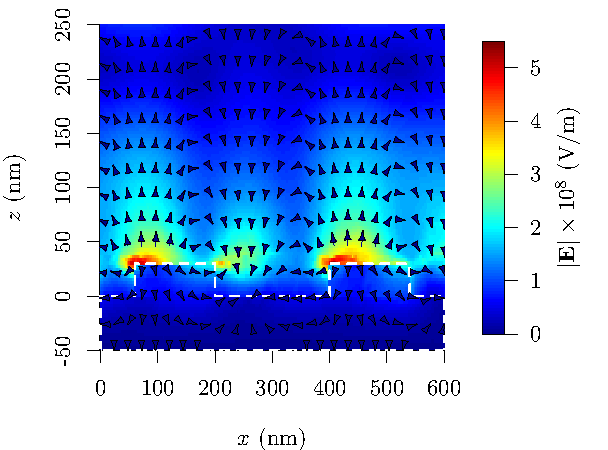
\includegraphics[]{figure-fieldplot-SPPonZigzag.pdf}
\centering \caption[The $\mathbf{E}$ field plot of a SPP excited by TE radiation.]{The $\mathbf{E}$ field plot of a SPP excited by TE radiation found in figure \ref{fig:anglescan}, obtained by FEM. The colour scale shows the magnitude of the electric vector, $\mathbf{E}$, for a cross section of the zigzag grating, in the plane of SPP propagation ($\parallel$ to $\mathbf{\hat{x}}$). The arrows show the direction of the electric vector over space. The electric field phase chosen for this travelling wave is arbitrary.\label{fig:zzfield-plot-expt}}
\end{figure}

Using the fitted FEM model, the magnitude of the electric field in the $xz$ plane is plotted for this SPP mode in figure \ref{fig:zzfield-plot-expt}. The electric field is evanescently confined to the surface with the field maximum occurring near the top, flat surface of the zigzags at $z=d=29.9\: \nano\metre$ and exponentially decaying away into both the air and the metal. The SPP for this wavelength and angle propagates along the zigzag with a wavevector given by $k_{SPP}=nk_0 \sin \theta - k_{gx}=1.67k_{gx}$, corresponding to a SPP wavelength of $\lambda_{SPP}=358\:\nano\metre$. The plane of intersection and temporal phase of the wave is arbitrarily and chosen for the figure as $y=70\:\nano\metre$ and $0^\circ$ phase, respectively. The propagation of the SPP along the zigzag, rather than over the grooves, has important consequences for the band structure for SPPs on this type of surface, and will be discussed in section \ref{sec:bandgap-character}.

It is desirable to fully confirm the coupling conditions outlined in equation \ref{eq:zz-tecoupling} for other odd-order diffracted modes, rather than just the $\pm\mathbf{k}_{gx}$ scattered SPP. By embedding a zigzag grating in a higher refractive index, such as glass, we are able to access the $+3\mathbf{k}_{gx}$ scattered SPP using visible frequency radiation.
The experimentally obtained dispersion of the SPPs on the glass/metal interface is mapped as a function of in plane wavevector, $\mathbf{k}_{gx}$, by varying the polar angle $\theta$ and angular frequency, $\omega$, using a polarised, collimated, monochromatic beam, produced by a white light source together with a spectrometer, in the wavelength range $400 < \lambda_0 < 850$ nm.
The reflectivity of incident TE polarised light at $\phi = 0^\circ$ is shown in figure \ref{fig:shallowzz-dispersion-expt}. 
\begin{figure}
\begin{center}
\subfigure[]{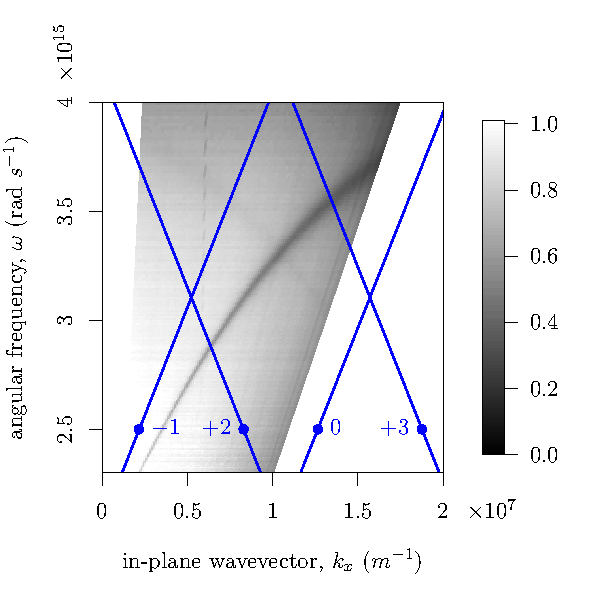
\includegraphics[width=0.49\linewidth]{figure-TEdispersion-symZZ-Exp}\label{fig:shallowzz-dispersion-expt}}
\subfigure[]{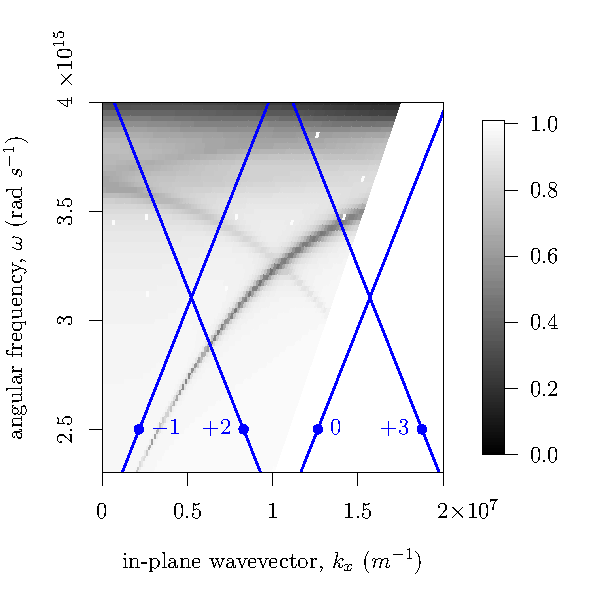
\includegraphics[width=0.49\linewidth]{figure-TEdispersion-symZZ-HFSS}\label{fig:shallowzz-dispersion-theory}}
\caption[SPP dispersion on a zigzag grating in glass measured using TE polarised light.]{(a) Experimental data and (b) numerically modelled results of the TE polarised reflectivity as a function of in-plane wavevector and angular frequency, mapping the SPP dispersion on a zigzag grating in glass. \color{blue}Blue \color{black} lines show the positions of diffracted light lines scattered by $m\mathbf{k}_{gx}$, where $m = −1, +2, 0, +3$.}
\end{center}
\end{figure}

With the grating embedded in glass two Bragg-scattered SPP dispersion curves are observed for this polarisation case. One originates at $-\mathbf{k}_{gx}$ and the other at $+3\mathbf{k}_{gx}$. These odd-order diffracted SPPs are excited by TE polarised light. There is no evidence of a SPP dispersion curve from a $+2\mathbf{k}_{gx}$ scattering event as, on a zigzag grating, it is not excited by TE polarised light as predicted by equation \ref{eq:zz-tecoupling}. Using the fitted parameters from figure \ref{fig:anglescan}, the dispersion plots were reproduced from FEM modelling and found to be in good agreement and are shown in figure \ref{fig:shallowzz-dispersion-theory}. The small difference between the model asymptotic limits of the SPPs and experiment may be attributed to the differences between the dielectric function of silver used for the model \cite{Nash1996} and our experimental sample. 

In summary, the SPPs are shown to be excited on the zigzag grating, with TE polarised light coupling to the odd-order Bragg scattered SPPs. The dispersion of the SPPs has been mapped for the two cases of the grating in air and in glass, and agrees well with a numerical model. No even-order modes are observed when the sample is illuminated with TE polarised light. There is no excitation of odd-order modes with TM polarised light.

\subsection{Transverse Magnetic Coupling\label{sec:TMexciatation}}

The observation of even-order Bragg scattered SPP modes coupled to by TM radiation is expected from the allowed charge distributions examined in section \ref{sec:zztheory}. For our sample, the experimental observation of this mode is difficult, as the zigzag grating is not optimally coupled to the SPP due to shallowing of the grating during fabrication, and the even-ordered diffraction is also very weak, only mediated by multiple scattering processes of $\pm \mathbf{k}_{gx}$.

To investigate the weak coupling of TM polarised light to the $+2\mathbf{k}_{gx}$ SPP, spectral plots are analysed for a range of angles for which, theoretically, only the  $2\mathbf{k}_{gx}$ SPP can be present. A zigzag grating in air was investigated over an angle range of ($39^\circ<\theta<55^\circ$), to remove the ambiguity of which SPP mode is under observation. Comparison to the TE reflectivity, which should not couple to the SPP, further helps identify the mode. An example spectrum for both TE and TM polarised illumination at $\theta=53^\circ$ is shown in figure \ref{fig:zz2ndordermodesSpectraAt53Degrees}. There is a clear broad absorption of the light in the TM case which is missing from the TE case, reducing the reflectivity by approximately 7\%. 

\begin{figure}
\begin{center}
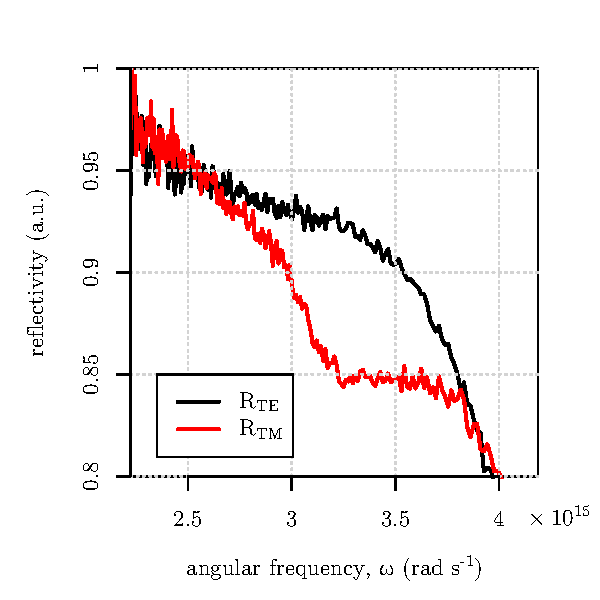
\includegraphics{2nd-order-mode/figure-TM-2ndorder-mode-spectra-exp.pdf}
\caption[An example experimental reflectivity plot for TE and TM polarised light in the visible range at a fixed polar angle of $\theta=53^\circ$.]{An example experimental reflectivity plot for TE and TM polarised light in the visible range at a fixed polar angle of $\theta=53^\circ$. The broad absorption in the TM case is attributed to the weak excitation of a $+2\mathbf{k}_{gx}$ scattered SPP. \label{fig:zz2ndordermodesSpectraAt53Degrees}}
\end{center}
\end{figure}

\begin{figure}
\begin{center}
\subfigure[]{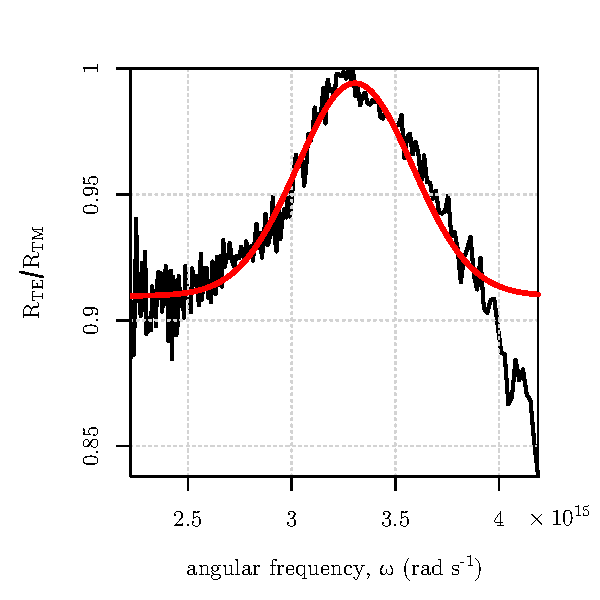
\includegraphics[width=0.49\linewidth]{2nd-order-mode/figure-TM-2ndorder-mode-RssDivRpp-exp}\label{fig:RppDivRss}}
\subfigure[]{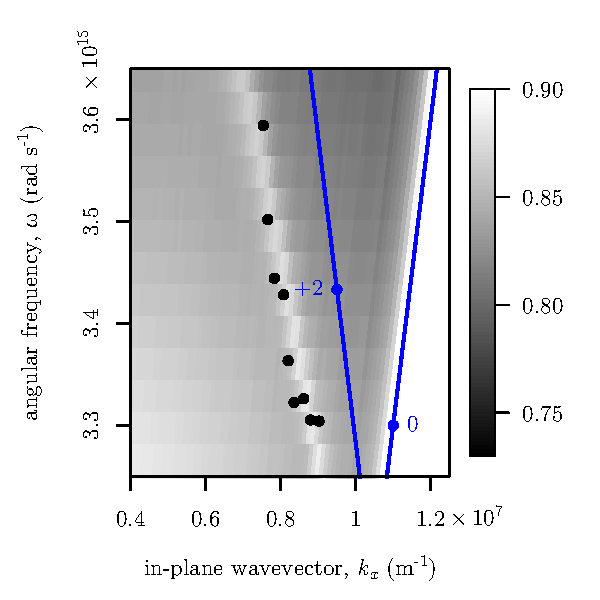
\includegraphics[width=0.49\linewidth]{2nd-order-mode/figure-zigzag-air-secondordermode-theoryAndExperiment-Rpp}\label{fig:Plot2ndOrderDispersionComparison}}
\caption[An example spectral plot and fit at $\theta=53^\circ$ for the TM reflectivity normalised to the TE reflectivity, and comparison to theory.]{(a) An example spectral plot and fit at $\theta=53^\circ$ for the TM reflectivity normalised to the TE reflectivity. (b) comparison between theory (greyscale) and experiment (black points) for a range of angles ($39^\circ<\theta<55^\circ$).}
\end{center}
\end{figure}

Both the TE and TM reflectivity drop at higher frequencies due to the UV absorption inherent in the optical response of silver. To remove this high frequency absorption and better judge the position of the broad reflectivity discontinuity associated with a weakly coupled SPP, the TE and TM reflectivity may be normalized with respect to each other. The TE reflectivity spectra, containing no observed SPP modes but containing the higher frequency absorption of silver, may be used to normalize the TM data and remove the high frequency silver absorption. This allows a greater accuracy in the determination of the broad TM coupled SPP mode's position in frequency, which is judged by the fitting of a Gaussian curve to the local maximum of the normalized reflectivity in figure \ref{fig:RppDivRss}.  To further confirm that this reflectivity anomaly is due to the weak excitation of the $+2\mathbf{k}_{gx}$ scattered SPP, the dispersion of this mode in frequency for the angle range $39^\circ<\theta<55^\circ$ is plotted on the modelled dispersion of the 2$^{nd}$ order mode in figure \ref{fig:Plot2ndOrderDispersionComparison}, obtained from the same FEM model that showed excellent agreement for the TE case in figure \ref{fig:TEdiseprsionInAir}. The SPP mode dispersion is found to be in good agreement with the theoretical prediction for the $+2\mathbf{k}_{gx}$ scattered SPP, and we conclude that this 2$^{nd}$ order mode is excited by TM polarised radiation, and is not excited by TE polarised light, in agreement with section \ref{sec:zztheory}.

\begin{figure}
\begin{center}
\subfigure[]{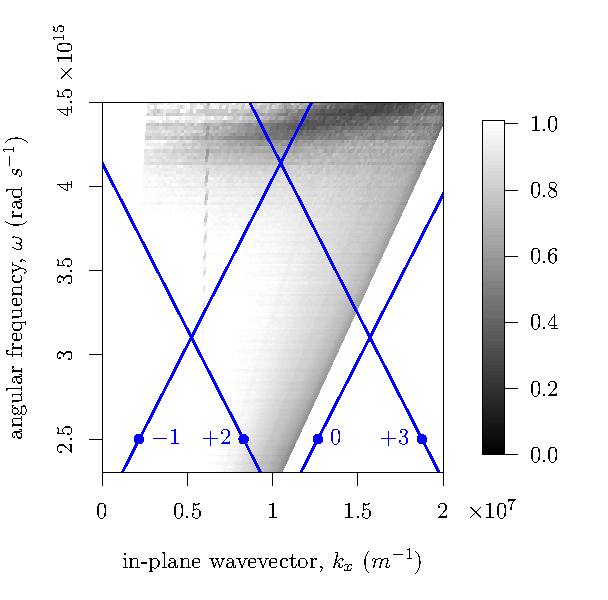
\includegraphics[width=0.45\linewidth]{figure-TMdispersion-symZZ-Exp}\label{fig:shallowzz-dispersion-TM-expt}}
\subfigure[]{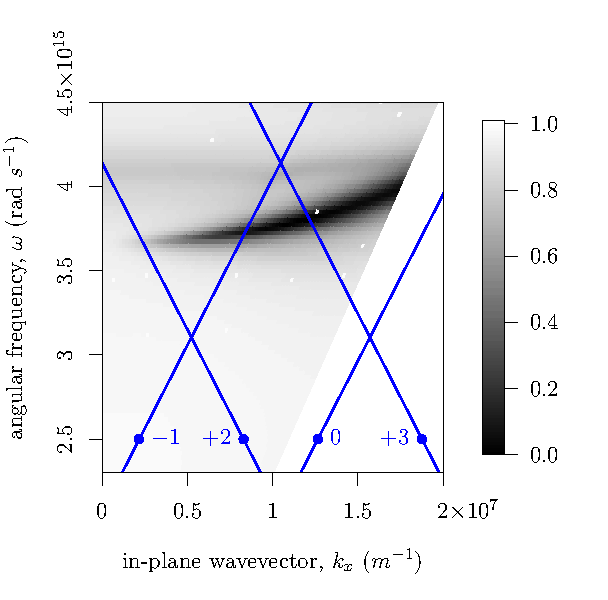
\includegraphics[width=0.45\linewidth]{figure-TMdispersion-symZZ-HFSS}\label{fig:shallowzz-dispersion-TM-theory}}
\caption[SPP dispersion on a zigzag grating in glass measured using TM polarised light.]{Experimental data of TM polarised reflectivity as a function of in-plane wavevector and angular frequency, mapping the SPP dispersion on a zigzag grating in glass. \color{blue}Blue \color{black} lines show the positions of diffracted light lines scattered by $m\mathbf{k}_{gx}$, where $m = −1, +2, 0, +3$. \label{fig:shallowzz-dispersion-TM-both}}
\end{center}
\end{figure}

Figure \ref{fig:shallowzz-dispersion-TM-both} shows the dispersion of the SPPs on the zigzag grating embedded in glass and mapped by using TM polarised light, obtained both experimentally and using FEM modelling. The only noticeable feature is a band of low reflectivity at high frequency, which does not appear to be associated with any of the in-plane diffracted light lines. This absorption of light is due to the excitation of a SPP that has been scattered by an out-of-plane grating vector, ($\mathbf{k}_{gy}$), and is observed as a flat parabolic curve. The explanation of this SPP band's shape for out-of-plane scattered SPPs intersecting the plane of incidence can be found previously in chapter \ref{c:backgroundtheory}. Both the experimental and theoretical figures show this band, although the experimental band lies at a higher frequency compared to the theoretical curve, due to the difference in the metal's dielectric function between that of the experimental sample and the values used for FEM. In the experimental case, this frequency is at the limit of the monochromator's spectral resolution, and so the signal to noise ratio is lower than for previous plots.

This out-of-plane SPP mode lies significantly removed from the diffracted light line for the $\pm \mathbf{k}_{gy}$ light cone, which is not plotted as it occurs at a higher frequency than the displayed spectral range. Comparing this difference, $\Delta k_{x}$, for in-plane modes observed under TE illumination, the observation of a $\mathbf{k}_{gy}$ scattered SPP mode with a large enough $\Delta k_{y}$ to be observed suggests a high level of anisotropic dispersion of the SPP in the $\mathbf{k}_x$ and $\mathbf{k}_y$ directions. This will be discussed further in section \ref{sec:anisotropic}.

In summary, the observation of weak even-scattered SPPs excited by TM polarised light has been demonstrated experimentally. To facilitate stronger coupling by even-order scattered SPPs and TM polarised light, an even $\mathbf{k}_{gx}$ component may to be added to the zigzag profile, but this would remove the mirror symmetry of the grating and the polarisation selectivity would be destroyed. This will be discussed further in chapter \ref{c:azigzag}. An out-of-plane SPP associated with $\pm \mathbf{k}_{gy}$ has also been observed, indicating that the SPP dispersion in the $\hat{\mathbf{y}}$ direction is significantly perturbed  from the in-plane ($\hat{\mathbf{y}}$) dispersion case. This anisotropic propagation of SPPs will be discussed further in section \ref{sec:anisotropic}.

\section{Band Structure of SPPs on a Zigzag Grating\label{sec:bandgap-character}}
The formation of SPP band-gaps relies on the ability for a propagating SPP mode to Bragg scatter  and interfere with its counter-propagating self \cite{Barnes1995,Barnes1996}. This interference forms two possible SPP standing waves on the surface of the grating, which will typically have two possible field solutions, with the fields of one solution spatially shifted by $\lambda_{gx}/4$ with respect to the other. Since only diffracted SPPs are observed in the light-cone, the minimum momentum by which a SPP must scatter to intersect an equivalent counter-propagating mode, and still be able to couple to light and be observed, is a total of $2\mathbf{k}_{gx}$.

On traditional surface-relief gratings, the positions of the standing wave anti-nodes correspond to induced surface charge on the grating grooves. The two possible standing waves will cause the surface charge density to sit in different arrangements per solution which will, in general, sit charge in different potentials. This means that the energy of the two standing wave solutions will differ, with no propagating SPPs between the two energies due to destructive inference. This is the essence of plasmonic band-gap formation.

On a zigzag grating, the SPPs propagating along the $\mathbf{k}_{gx}$ direction do not run over surface relief grooves, but follow the zigzag shape along the surface. The two possible standing waves which form when counter-propagating SPPs interact will differ in energy by an amount determined by the zigzag structure of the surface and not the shape or depth of the grooves. The positions of the standing wave anti-nodes correspond to induced surface charge along the zigzag, and by consideration of these charge arrangements, the band-gap character of zigzag gratings may be inferred.

\subsection{Band-Gaps at $k_x=0$}
For a zigzag grating with a periodicity of $\lambda_g= 600$ nm in air, the $\pm\mathbf{k}_{gx}$ scattered SPPs meet at $k_x=0$ within the visible frequency range. An experimentally obtained iso-frequency contour for these modes is displayed in figure \ref{fig:no-interacting-scattergram}. The dark bands of low reflectivity map the SPP mode positions. At $k_x=0$ the $+1\mathbf{k}_{gx}$ and $-1\mathbf{k}_{gx}$ SPP contours cross, and no significant perturbation of these contours is observed. No band-gap is detected at the mode intersections. 
\begin{figure}
\begin{center}
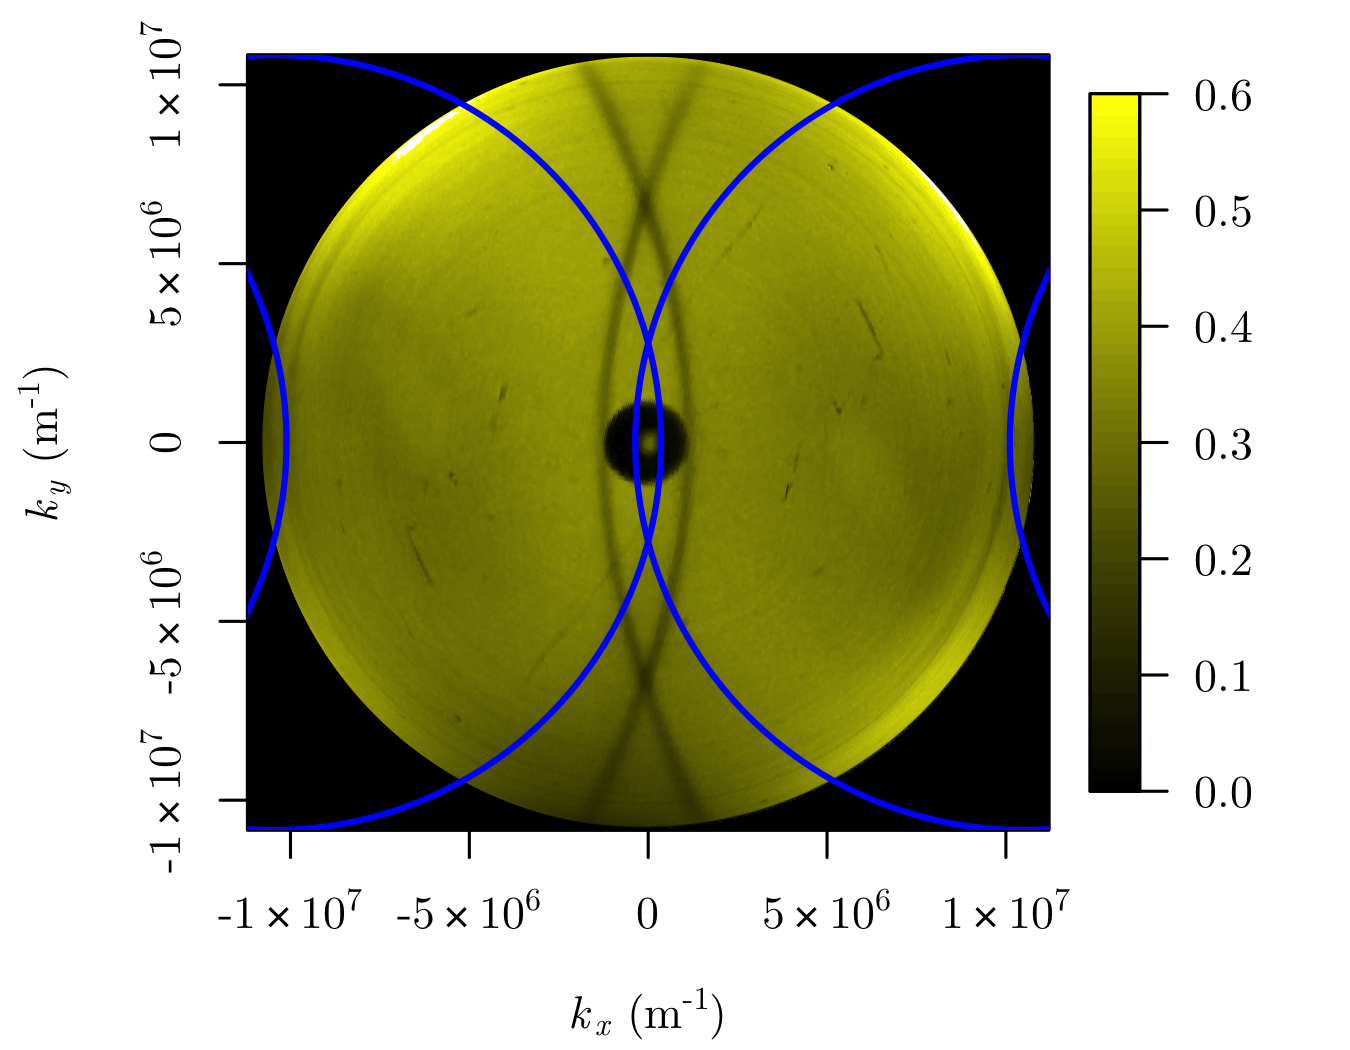
\includegraphics[width=0.7\linewidth]{scattergrams/figure-580nm-scattergram-withaxes.png}
\end{center}
\caption[An iso-frequency scattergram mapping $k$-space contours for a 600 nm zigzag grating for an energy of 2.14 eV]{An iso-frequency scattergram mapping $k$-space contours for a 600 nm zigzag grating for an energy of 2.14 eV ($\lambda_0=580$ nm). The blue circles indicate the $\pm k_{gx}$ scattered light circles.\label{fig:no-interacting-scattergram}}
\end{figure}
The lack of interaction of these modes along $k_x=0$ is consistent with the known scattering properties of a zigzag grating. The grating profile, being totally described by odd functions, contain no significant $2k_{gx}$ components. The result of which is that a SPP must undergo multiple scattering processes of $\pm n \mathbf{k}_{gx}$, where $n$ is odd, in order to diffract and intersect other SPP modes. These multiple scattering processes are very weak, and result in such a small perturbation of the modes as they intersect in $k$-space that no band-gap is observed experimentally. 

While no band-gap is measured, the existence of a band-gap in this case is not forbidden. Figure \ref{fig:zzbandgapcartoon-kx0} shows a diagrammatic representation of the expected locations of nodes and anti-nodes at $k_x=0$ for the $xy$ plane. As previously mentioned, the SPPs on zigzag gratings run along the zigzag, not over the grooves. For two SPP standing waves to be energetically dissimilar, the pertinent consideration is the field arrangements along the zigzag structure itself, which is why we consider the $xy$ plane. The wavevector of this standing wave is half that of the Bragg vector by which the SPPs have scattered, in this case $2\mathbf{k}_{gx}/2$, leading to a standing wave with the periodicity of $\lambda_{gx}$. 
\begin{figure}
\begin{center}
\subfigure[]{% Created by tikzDevice version 0.6.2-92-0ad2792 on 2012-12-18 15:43:19
% !TEX encoding = UTF-8 Unicode
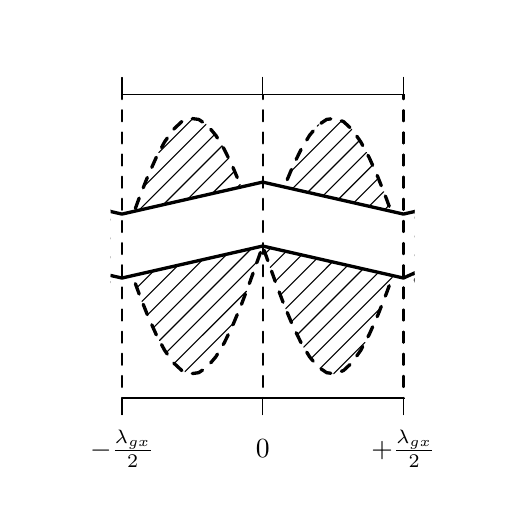
\begin{tikzpicture}[x=1pt,y=1pt]
\definecolor[named]{fillColor}{rgb}{1.00,1.00,1.00}
\path[use as bounding box,fill=fillColor,fill opacity=0.00] (0,0) rectangle (169.83,169.83);
\begin{scope}
\path[clip] ( 30.00, 36.00) rectangle (139.83,145.83);
\definecolor[named]{drawColor}{rgb}{0.00,0.00,0.00}

\path[draw=drawColor,line width= 1.2pt,dash pattern=on 4pt off 4pt ,line join=round,line cap=round] (  0.00, 51.16) --
	(  0.17, 50.88) --
	(  3.25, 47.23) --
	(  6.33, 45.16) --
	(  9.41, 44.74) --
	( 12.50, 45.99) --
	( 15.58, 48.87) --
	( 18.66, 53.26) --
	( 21.74, 59.02) --
	( 24.82, 65.93) --
	( 27.90, 73.74) --
	( 30.99, 82.17) --
	( 34.07, 90.92) --
	( 37.15, 99.67) --
	( 40.23,108.10) --
	( 43.31,115.91) --
	( 46.40,122.82) --
	( 49.48,128.57) --
	( 52.56,132.97) --
	( 55.64,135.84) --
	( 58.72,137.09) --
	( 61.80,136.67) --
	( 64.89,134.60) --
	( 67.97,130.95) --
	( 71.05,125.85) --
	( 74.13,119.49) --
	( 77.21,112.10) --
	( 80.29,103.94) --
	( 83.38, 95.31) --
	( 86.46, 86.52) --
	( 89.54, 77.89) --
	( 92.62, 69.73) --
	( 95.70, 62.34) --
	( 98.79, 55.98) --
	(101.87, 50.88) --
	(104.95, 47.23) --
	(108.03, 45.16) --
	(111.11, 44.74) --
	(114.19, 45.99) --
	(117.28, 48.87) --
	(120.36, 53.26) --
	(123.44, 59.02) --
	(126.52, 65.93) --
	(129.60, 73.74) --
	(132.68, 82.17) --
	(135.77, 90.92) --
	(138.85, 99.67) --
	(141.93,108.10) --
	(145.01,115.91) --
	(148.09,122.82) --
	(151.18,128.57) --
	(154.26,132.97) --
	(157.34,135.84) --
	(160.42,137.09) --
	(163.50,136.67) --
	(166.58,134.60) --
	(169.67,130.95) --
	(169.83,130.67);
\end{scope}
\begin{scope}
\path[clip] ( 30.00, 36.00) rectangle (139.83,145.83);
\definecolor[named]{drawColor}{rgb}{0.00,0.00,0.00}

\path[draw=drawColor,line width= 1.2pt,dash pattern=on 4pt off 4pt ,line join=round,line cap=round] (  0.00,130.67) --
	(  0.17,130.95) --
	(  3.25,134.60) --
	(  6.33,136.67) --
	(  9.41,137.09) --
	( 12.50,135.84) --
	( 15.58,132.97) --
	( 18.66,128.57) --
	( 21.74,122.82) --
	( 24.82,115.91) --
	( 27.90,108.10) --
	( 30.99, 99.67) --
	( 34.07, 90.92) --
	( 37.15, 82.17) --
	( 40.23, 73.74) --
	( 43.31, 65.93) --
	( 46.40, 59.02) --
	( 49.48, 53.26) --
	( 52.56, 48.87) --
	( 55.64, 45.99) --
	( 58.72, 44.74) --
	( 61.80, 45.16) --
	( 64.89, 47.23) --
	( 67.97, 50.88) --
	( 71.05, 55.98) --
	( 74.13, 62.34) --
	( 77.21, 69.73) --
	( 80.29, 77.89) --
	( 83.38, 86.52) --
	( 86.46, 95.31) --
	( 89.54,103.94) --
	( 92.62,112.10) --
	( 95.70,119.49) --
	( 98.79,125.85) --
	(101.87,130.95) --
	(104.95,134.60) --
	(108.03,136.67) --
	(111.11,137.09) --
	(114.19,135.84) --
	(117.28,132.97) --
	(120.36,128.57) --
	(123.44,122.82) --
	(126.52,115.91) --
	(129.60,108.10) --
	(132.68, 99.67) --
	(135.77, 90.92) --
	(138.85, 82.17) --
	(141.93, 73.74) --
	(145.01, 65.93) --
	(148.09, 59.02) --
	(151.18, 53.26) --
	(154.26, 48.87) --
	(157.34, 45.99) --
	(160.42, 44.74) --
	(163.50, 45.16) --
	(166.58, 47.23) --
	(169.67, 50.88) --
	(169.83, 51.16);

\path[draw=drawColor,line width= 0.4pt,line join=round,line cap=round] (  0.00,124.99) -- ( 11.33,136.31);

\path[draw=drawColor,line width= 0.4pt,line join=round,line cap=round] (  0.00,118.17) -- ( 15.17,133.34);

\path[draw=drawColor,line width= 0.4pt,line join=round,line cap=round] (  0.00,111.36) -- ( 18.06,129.42);

\path[draw=drawColor,line width= 0.4pt,line join=round,line cap=round] (  0.00,104.55) -- ( 20.53,125.08);

\path[draw=drawColor,line width= 0.4pt,line join=round,line cap=round] (  0.00, 97.73) -- ( 22.77,120.50);

\path[draw=drawColor,line width= 0.4pt,line join=round,line cap=round] (  0.00, 90.92) -- ( 24.87,115.79);

\path[draw=drawColor,line width= 0.4pt,line join=round,line cap=round] (  0.00, 84.10) -- (  6.81, 90.92);

\path[draw=drawColor,line width= 0.4pt,line join=round,line cap=round] (  6.81, 90.92) -- ( 26.80,110.90);

\path[draw=drawColor,line width= 0.4pt,line join=round,line cap=round] (  0.00, 77.29) -- ( 13.63, 90.92);

\path[draw=drawColor,line width= 0.4pt,line join=round,line cap=round] ( 13.63, 90.92) -- ( 28.68,105.97);

\path[draw=drawColor,line width= 0.4pt,line join=round,line cap=round] ( 47.40,124.69) -- ( 59.67,136.96);

\path[draw=drawColor,line width= 0.4pt,line join=round,line cap=round] (  0.00, 70.48) -- ( 20.44, 90.92);

\path[draw=drawColor,line width= 0.4pt,line join=round,line cap=round] ( 20.44, 90.92) -- ( 30.51,100.98);

\path[draw=drawColor,line width= 0.4pt,line join=round,line cap=round] ( 41.93,112.41) -- ( 64.43,134.91);

\path[draw=drawColor,line width= 0.4pt,line join=round,line cap=round] (  0.00, 63.66) -- ( 27.25, 90.92);

\path[draw=drawColor,line width= 0.4pt,line join=round,line cap=round] ( 27.25, 90.92) -- ( 32.29, 95.96);

\path[draw=drawColor,line width= 0.4pt,line join=round,line cap=round] ( 37.81,101.47) -- ( 67.66,131.32);

\path[draw=drawColor,line width= 0.4pt,line join=round,line cap=round] (  0.00, 56.85) -- ( 34.07, 90.92);

\path[draw=drawColor,line width= 0.4pt,line join=round,line cap=round] ( 34.07, 90.92) -- ( 34.07, 90.92);

\path[draw=drawColor,line width= 0.4pt,line join=round,line cap=round] ( 34.07, 90.92) -- ( 70.28,127.13);

\path[draw=drawColor,line width= 0.4pt,line join=round,line cap=round] (  0.48, 50.52) -- ( 30.33, 80.36);

\path[draw=drawColor,line width= 0.4pt,line join=round,line cap=round] ( 35.84, 85.88) -- ( 40.88, 90.92);

\path[draw=drawColor,line width= 0.4pt,line join=round,line cap=round] ( 40.88, 90.92) -- ( 72.61,122.64);

\path[draw=drawColor,line width= 0.4pt,line join=round,line cap=round] (  3.71, 46.93) -- ( 26.20, 69.43);

\path[draw=drawColor,line width= 0.4pt,line join=round,line cap=round] ( 37.63, 80.85) -- ( 47.70, 90.92);

\path[draw=drawColor,line width= 0.4pt,line join=round,line cap=round] ( 47.70, 90.92) -- ( 74.76,117.98);

\path[draw=drawColor,line width= 0.4pt,line join=round,line cap=round] (  8.46, 44.87) -- ( 20.74, 57.15);

\path[draw=drawColor,line width= 0.4pt,line join=round,line cap=round] ( 39.45, 75.86) -- ( 54.51, 90.92);

\path[draw=drawColor,line width= 0.4pt,line join=round,line cap=round] ( 54.51, 90.92) -- ( 76.77,113.17);

\path[draw=drawColor,line width= 0.4pt,line join=round,line cap=round] ( 41.34, 70.93) -- ( 61.32, 90.92);

\path[draw=drawColor,line width= 0.4pt,line join=round,line cap=round] ( 61.32, 90.92) -- ( 78.66,108.26);

\path[draw=drawColor,line width= 0.4pt,line join=round,line cap=round] (104.63,134.23) -- (105.13,134.72);

\path[draw=drawColor,line width= 0.4pt,line join=round,line cap=round] ( 43.27, 66.05) -- ( 68.14, 90.92);

\path[draw=drawColor,line width= 0.4pt,line join=round,line cap=round] ( 68.14, 90.92) -- ( 80.52,103.30);

\path[draw=drawColor,line width= 0.4pt,line join=round,line cap=round] ( 94.98,117.76) -- (113.39,136.17);

\path[draw=drawColor,line width= 0.4pt,line join=round,line cap=round] ( 45.36, 61.33) -- ( 74.95, 90.92);

\path[draw=drawColor,line width= 0.4pt,line join=round,line cap=round] ( 74.95, 90.92) -- ( 82.32, 98.28);

\path[draw=drawColor,line width= 0.4pt,line join=round,line cap=round] ( 90.49,106.46) -- (117.13,133.10);

\path[draw=drawColor,line width= 0.4pt,line join=round,line cap=round] ( 47.60, 56.76) -- ( 81.76, 90.92);

\path[draw=drawColor,line width= 0.4pt,line join=round,line cap=round] ( 81.76, 90.92) -- ( 84.10, 93.25);

\path[draw=drawColor,line width= 0.4pt,line join=round,line cap=round] ( 86.62, 95.78) -- (119.97,129.12);

\path[draw=drawColor,line width= 0.4pt,line join=round,line cap=round] ( 50.07, 52.41) -- ( 82.93, 85.27);

\path[draw=drawColor,line width= 0.4pt,line join=round,line cap=round] ( 85.87, 88.21) -- ( 88.58, 90.92);

\path[draw=drawColor,line width= 0.4pt,line join=round,line cap=round] ( 88.58, 90.92) -- (122.41,124.75);

\path[draw=drawColor,line width= 0.4pt,line join=round,line cap=round] ( 52.96, 48.49) -- ( 79.04, 74.56);

\path[draw=drawColor,line width= 0.4pt,line join=round,line cap=round] ( 87.65, 83.18) -- ( 95.39, 90.92);

\path[draw=drawColor,line width= 0.4pt,line join=round,line cap=round] ( 95.39, 90.92) -- (124.63,120.15);

\path[draw=drawColor,line width= 0.4pt,line join=round,line cap=round] ( 56.81, 45.52) -- ( 74.49, 63.20);

\path[draw=drawColor,line width= 0.4pt,line join=round,line cap=round] ( 89.45, 78.16) -- (102.20, 90.92);

\path[draw=drawColor,line width= 0.4pt,line join=round,line cap=round] (102.20, 90.92) -- (126.71,115.42);

\path[draw=drawColor,line width= 0.4pt,line join=round,line cap=round] ( 91.31, 73.21) -- (109.02, 90.92);

\path[draw=drawColor,line width= 0.4pt,line join=round,line cap=round] (109.02, 90.92) -- (128.64,110.54);

\path[draw=drawColor,line width= 0.4pt,line join=round,line cap=round] ( 93.22, 68.30) -- (115.83, 90.92);

\path[draw=drawColor,line width= 0.4pt,line join=round,line cap=round] (115.83, 90.92) -- (130.52,105.60);

\path[draw=drawColor,line width= 0.4pt,line join=round,line cap=round] (148.51,123.60) -- (161.82,136.90);

\path[draw=drawColor,line width= 0.4pt,line join=round,line cap=round] ( 95.22, 63.49) -- (122.65, 90.92);

\path[draw=drawColor,line width= 0.4pt,line join=round,line cap=round] (122.65, 90.92) -- (132.34,100.61);

\path[draw=drawColor,line width= 0.4pt,line join=round,line cap=round] (143.30,111.57) -- (166.43,134.70);

\path[draw=drawColor,line width= 0.4pt,line join=round,line cap=round] ( 97.39, 58.85) -- (129.46, 90.92);

\path[draw=drawColor,line width= 0.4pt,line join=round,line cap=round] (129.46, 90.92) -- (134.12, 95.58);

\path[draw=drawColor,line width= 0.4pt,line join=round,line cap=round] (139.22,100.67) -- (169.59,131.04);

\path[draw=drawColor,line width= 0.4pt,line join=round,line cap=round] ( 99.75, 54.39) -- (135.49, 90.14);

\path[draw=drawColor,line width= 0.4pt,line join=round,line cap=round] (135.90, 90.54) -- (136.27, 90.92);

\path[draw=drawColor,line width= 0.4pt,line join=round,line cap=round] (136.27, 90.92) -- (169.83,124.48);

\path[draw=drawColor,line width= 0.4pt,line join=round,line cap=round] (102.41, 50.24) -- (131.73, 79.56);

\path[draw=drawColor,line width= 0.4pt,line join=round,line cap=round] (137.67, 85.50) -- (143.09, 90.92);

\path[draw=drawColor,line width= 0.4pt,line join=round,line cap=round] (143.09, 90.92) -- (169.83,117.66);

\path[draw=drawColor,line width= 0.4pt,line join=round,line cap=round] (105.71, 46.72) -- (127.57, 68.59);

\path[draw=drawColor,line width= 0.4pt,line join=round,line cap=round] (139.46, 80.48) -- (149.90, 90.92);

\path[draw=drawColor,line width= 0.4pt,line join=round,line cap=round] (149.90, 90.92) -- (169.83,110.85);

\path[draw=drawColor,line width= 0.4pt,line join=round,line cap=round] (110.61, 44.81) -- (121.85, 56.06);

\path[draw=drawColor,line width= 0.4pt,line join=round,line cap=round] (141.29, 75.49) -- (156.71, 90.92);

\path[draw=drawColor,line width= 0.4pt,line join=round,line cap=round] (156.71, 90.92) -- (169.83,104.04);

\path[draw=drawColor,line width= 0.4pt,line join=round,line cap=round] (143.18, 70.57) -- (163.53, 90.92);

\path[draw=drawColor,line width= 0.4pt,line join=round,line cap=round] (163.53, 90.92) -- (169.83, 97.22);

\path[draw=drawColor,line width= 0.4pt,line join=round,line cap=round] (145.12, 65.69) -- (169.83, 90.41);

\path[draw=drawColor,line width= 0.4pt,line join=round,line cap=round] (147.22, 60.98) -- (169.83, 83.60);

\path[draw=drawColor,line width= 0.4pt,line join=round,line cap=round] (149.48, 56.43) -- (169.83, 76.78);

\path[draw=drawColor,line width= 0.4pt,line join=round,line cap=round] (151.98, 52.11) -- (169.83, 69.97);

\path[draw=drawColor,line width= 0.4pt,line join=round,line cap=round] (154.92, 48.25) -- (169.83, 63.16);

\path[draw=drawColor,line width= 0.4pt,line join=round,line cap=round] (158.87, 45.37) -- (169.83, 56.34);

\path[] (  0.00, 51.16) --
	(  0.17, 50.88) --
	(  3.25, 47.23) --
	(  6.33, 45.16) --
	(  9.41, 44.74) --
	( 12.50, 45.99) --
	( 15.58, 48.87) --
	( 18.66, 53.26) --
	( 21.74, 59.02) --
	( 24.82, 65.93) --
	( 27.90, 73.74) --
	( 30.99, 82.17) --
	( 34.07, 90.92) --
	( 37.15, 99.67) --
	( 40.23,108.10) --
	( 43.31,115.91) --
	( 46.40,122.82) --
	( 49.48,128.57) --
	( 52.56,132.97) --
	( 55.64,135.84) --
	( 58.72,137.09) --
	( 61.80,136.67) --
	( 64.89,134.60) --
	( 67.97,130.95) --
	( 71.05,125.85) --
	( 74.13,119.49) --
	( 77.21,112.10) --
	( 80.29,103.94) --
	( 83.38, 95.31) --
	( 86.46, 86.52) --
	( 89.54, 77.89) --
	( 92.62, 69.73) --
	( 95.70, 62.34) --
	( 98.79, 55.98) --
	(101.87, 50.88) --
	(104.95, 47.23) --
	(108.03, 45.16) --
	(111.11, 44.74) --
	(114.19, 45.99) --
	(117.28, 48.87) --
	(120.36, 53.26) --
	(123.44, 59.02) --
	(126.52, 65.93) --
	(129.60, 73.74) --
	(132.68, 82.17) --
	(135.77, 90.92) --
	(138.85, 99.67) --
	(141.93,108.10) --
	(145.01,115.91) --
	(148.09,122.82) --
	(151.18,128.57) --
	(154.26,132.97) --
	(157.34,135.84) --
	(160.42,137.09) --
	(163.50,136.67) --
	(166.58,134.60) --
	(169.67,130.95) --
	(169.83,130.67);

\path[] (169.83, 90.92) --
	(  0.00, 90.92);

\path[] (  0.00,130.67) --
	(  0.17,130.95) --
	(  3.25,134.60) --
	(  6.33,136.67) --
	(  9.41,137.09) --
	( 12.50,135.84) --
	( 15.58,132.97) --
	( 18.66,128.57) --
	( 21.74,122.82) --
	( 24.82,115.91) --
	( 27.90,108.10) --
	( 30.99, 99.67) --
	( 34.07, 90.92) --
	( 37.15, 82.17) --
	( 40.23, 73.74) --
	( 43.31, 65.93) --
	( 46.40, 59.02) --
	( 49.48, 53.26) --
	( 52.56, 48.87) --
	( 55.64, 45.99) --
	( 58.72, 44.74) --
	( 61.80, 45.16) --
	( 64.89, 47.23) --
	( 67.97, 50.88) --
	( 71.05, 55.98) --
	( 74.13, 62.34) --
	( 77.21, 69.73) --
	( 80.29, 77.89) --
	( 83.38, 86.52) --
	( 86.46, 95.31) --
	( 89.54,103.94) --
	( 92.62,112.10) --
	( 95.70,119.49) --
	( 98.79,125.85) --
	(101.87,130.95) --
	(104.95,134.60) --
	(108.03,136.67) --
	(111.11,137.09) --
	(114.19,135.84) --
	(117.28,132.97) --
	(120.36,128.57) --
	(123.44,122.82) --
	(126.52,115.91) --
	(129.60,108.10) --
	(132.68, 99.67) --
	(135.77, 90.92) --
	(138.85, 82.17) --
	(141.93, 73.74) --
	(145.01, 65.93) --
	(148.09, 59.02) --
	(151.18, 53.26) --
	(154.26, 48.87) --
	(157.34, 45.99) --
	(160.42, 44.74) --
	(163.50, 45.16) --
	(166.58, 47.23) --
	(169.67, 50.88) --
	(169.83, 51.16);

\path[] (169.83, 90.92) --
	(  0.00, 90.92);
\definecolor[named]{fillColor}{rgb}{1.00,1.00,1.00}

\path[draw=drawColor,line width= 1.2pt,line join=round,line cap=round,fill=fillColor] ( 34.07, 79.36) --
	(  0.00, 87.10) --
	(  0.00,110.22) --
	( 34.07,102.47) --
	( 84.92,114.03) --
	(135.77,102.47) --
	(169.83,110.22) --
	(169.83, 94.85) --
	(135.77, 79.36) --
	( 84.92, 90.92) --
	cycle;
\end{scope}
\begin{scope}
\path[clip] (  0.00,  0.00) rectangle (169.83,169.83);
\definecolor[named]{drawColor}{rgb}{0.00,0.00,0.00}

\path[draw=drawColor,line width= 0.4pt,line join=round,line cap=round] ( 34.07, 36.00) -- (135.77, 36.00);

\path[draw=drawColor,line width= 0.4pt,line join=round,line cap=round] ( 34.07, 36.00) -- ( 34.07, 30.00);

\path[draw=drawColor,line width= 0.4pt,line join=round,line cap=round] ( 84.92, 36.00) -- ( 84.92, 30.00);

\path[draw=drawColor,line width= 0.4pt,line join=round,line cap=round] (135.77, 36.00) -- (135.77, 30.00);

\node[text=drawColor,anchor=base,inner sep=0pt, outer sep=0pt, scale=  1.00] at ( 34.07, 14.40) {$-\frac{\lambda_{gx}}{2}$};

\node[text=drawColor,anchor=base,inner sep=0pt, outer sep=0pt, scale=  1.00] at ( 84.92, 14.40) {$0$};

\node[text=drawColor,anchor=base,inner sep=0pt, outer sep=0pt, scale=  1.00] at (135.77, 14.40) {$+\frac{\lambda_{gx}}{2}$};

\path[draw=drawColor,line width= 0.4pt,line join=round,line cap=round] ( 34.07,145.83) -- (135.77,145.83);

\path[draw=drawColor,line width= 0.4pt,line join=round,line cap=round] ( 34.07,145.83) -- ( 34.07,151.83);

\path[draw=drawColor,line width= 0.4pt,line join=round,line cap=round] ( 84.92,145.83) -- ( 84.92,151.83);

\path[draw=drawColor,line width= 0.4pt,line join=round,line cap=round] (135.77,145.83) -- (135.77,151.83);
\end{scope}
\begin{scope}
\path[clip] ( 30.00, 36.00) rectangle (139.83,145.83);
\definecolor[named]{drawColor}{rgb}{0.00,0.00,0.00}

\path[draw=drawColor,line width= 0.8pt,dash pattern=on 4pt off 4pt ,line join=round,line cap=round] ( 34.07,  0.00) --
	( 34.07,169.83);

\path[draw=drawColor,line width= 0.8pt,dash pattern=on 4pt off 4pt ,line join=round,line cap=round] (135.77,  0.00) --
	(135.77,169.83);

\path[draw=drawColor,line width= 0.8pt,dash pattern=on 4pt off 4pt ,line join=round,line cap=round] ( 84.92,  0.00) --
	( 84.92,169.83);
\end{scope}
\end{tikzpicture}
\label{fig:zzbandgapcartoon-kx0A}}
\subfigure[]{% Created by tikzDevice version 0.6.2-92-0ad2792 on 2012-12-18 15:43:19
% !TEX encoding = UTF-8 Unicode
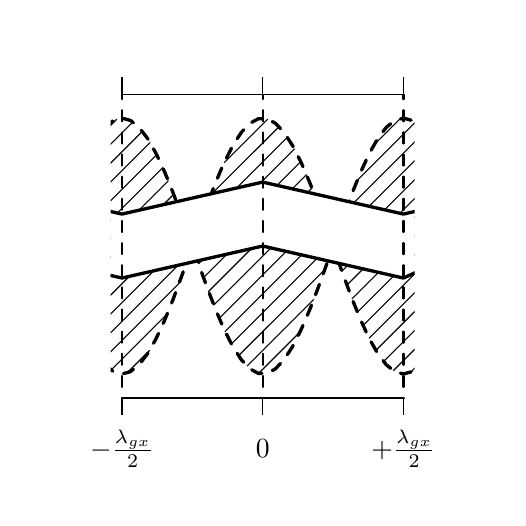
\begin{tikzpicture}[x=1pt,y=1pt]
\definecolor[named]{fillColor}{rgb}{1.00,1.00,1.00}
\path[use as bounding box,fill=fillColor,fill opacity=0.00] (0,0) rectangle (169.83,169.83);
\begin{scope}
\path[clip] ( 30.00, 36.00) rectangle (139.83,145.83);
\definecolor[named]{drawColor}{rgb}{0.00,0.00,0.00}

\path[draw=drawColor,line width= 1.2pt,dash pattern=on 4pt off 4pt ,line join=round,line cap=round] (  0.00, 67.41) --
	(  0.17, 67.80) --
	(  3.25, 75.80) --
	(  6.33, 84.34) --
	(  9.41, 93.12) --
	( 12.50,101.82) --
	( 15.58,110.12) --
	( 18.66,117.73) --
	( 21.74,124.37) --
	( 24.82,129.81) --
	( 27.90,133.83) --
	( 30.99,136.31) --
	( 34.07,137.14) --
	( 37.15,136.31) --
	( 40.23,133.83) --
	( 43.31,129.81) --
	( 46.40,124.37) --
	( 49.48,117.73) --
	( 52.56,110.12) --
	( 55.64,101.82) --
	( 58.72, 93.12) --
	( 61.80, 84.34) --
	( 64.89, 75.80) --
	( 67.97, 67.80) --
	( 71.05, 60.65) --
	( 74.13, 54.58) --
	( 77.21, 49.83) --
	( 80.29, 46.56) --
	( 83.38, 44.90) --
	( 86.46, 44.90) --
	( 89.54, 46.56) --
	( 92.62, 49.83) --
	( 95.70, 54.58) --
	( 98.79, 60.65) --
	(101.87, 67.80) --
	(104.95, 75.80) --
	(108.03, 84.34) --
	(111.11, 93.12) --
	(114.19,101.82) --
	(117.28,110.12) --
	(120.36,117.73) --
	(123.44,124.37) --
	(126.52,129.81) --
	(129.60,133.83) --
	(132.68,136.31) --
	(135.77,137.14) --
	(138.85,136.31) --
	(141.93,133.83) --
	(145.01,129.81) --
	(148.09,124.37) --
	(151.18,117.73) --
	(154.26,110.12) --
	(157.34,101.82) --
	(160.42, 93.12) --
	(163.50, 84.34) --
	(166.58, 75.80) --
	(169.67, 67.80) --
	(169.83, 67.41);
\end{scope}
\begin{scope}
\path[clip] ( 30.00, 36.00) rectangle (139.83,145.83);
\definecolor[named]{drawColor}{rgb}{0.00,0.00,0.00}

\path[draw=drawColor,line width= 1.2pt,dash pattern=on 4pt off 4pt ,line join=round,line cap=round] (  0.00,114.42) --
	(  0.17,114.03) --
	(  3.25,106.04) --
	(  6.33, 97.50) --
	(  9.41, 88.72) --
	( 12.50, 80.02) --
	( 15.58, 71.71) --
	( 18.66, 64.10) --
	( 21.74, 57.46) --
	( 24.82, 52.03) --
	( 27.90, 48.00) --
	( 30.99, 45.53) --
	( 34.07, 44.69) --
	( 37.15, 45.53) --
	( 40.23, 48.00) --
	( 43.31, 52.03) --
	( 46.40, 57.46) --
	( 49.48, 64.10) --
	( 52.56, 71.71) --
	( 55.64, 80.02) --
	( 58.72, 88.72) --
	( 61.80, 97.50) --
	( 64.89,106.04) --
	( 67.97,114.03) --
	( 71.05,121.19) --
	( 74.13,127.25) --
	( 77.21,132.01) --
	( 80.29,135.27) --
	( 83.38,136.93) --
	( 86.46,136.93) --
	( 89.54,135.27) --
	( 92.62,132.01) --
	( 95.70,127.25) --
	( 98.79,121.19) --
	(101.87,114.03) --
	(104.95,106.04) --
	(108.03, 97.50) --
	(111.11, 88.72) --
	(114.19, 80.02) --
	(117.28, 71.71) --
	(120.36, 64.10) --
	(123.44, 57.46) --
	(126.52, 52.03) --
	(129.60, 48.00) --
	(132.68, 45.53) --
	(135.77, 44.69) --
	(138.85, 45.53) --
	(141.93, 48.00) --
	(145.01, 52.03) --
	(148.09, 57.46) --
	(151.18, 64.10) --
	(154.26, 71.71) --
	(157.34, 80.02) --
	(160.42, 88.72) --
	(163.50, 97.50) --
	(166.58,106.04) --
	(169.67,114.03) --
	(169.83,114.42);

\path[draw=drawColor,line width= 0.4pt,line join=round,line cap=round] (  0.00,111.36) -- (  0.88,112.24);

\path[draw=drawColor,line width= 0.4pt,line join=round,line cap=round] (  0.00,104.55) -- (  2.75,107.30);

\path[draw=drawColor,line width= 0.4pt,line join=round,line cap=round] ( 24.35,128.90) -- ( 32.19,136.73);

\path[draw=drawColor,line width= 0.4pt,line join=round,line cap=round] (  0.00, 97.73) -- (  4.60,102.33);

\path[draw=drawColor,line width= 0.4pt,line join=round,line cap=round] ( 17.76,115.49) -- ( 38.02,135.75);

\path[draw=drawColor,line width= 0.4pt,line join=round,line cap=round] (  0.00, 90.92) -- (  6.39, 97.31);

\path[draw=drawColor,line width= 0.4pt,line join=round,line cap=round] ( 13.41,104.33) -- ( 41.43,132.35);

\path[draw=drawColor,line width= 0.4pt,line join=round,line cap=round] (  0.00, 84.10) -- (  6.81, 90.92);

\path[draw=drawColor,line width= 0.4pt,line join=round,line cap=round] (  6.81, 90.92) -- (  8.17, 92.27);

\path[draw=drawColor,line width= 0.4pt,line join=round,line cap=round] (  9.63, 93.74) -- ( 44.22,128.32);

\path[draw=drawColor,line width= 0.4pt,line join=round,line cap=round] (  0.00, 77.29) -- (  5.92, 83.21);

\path[draw=drawColor,line width= 0.4pt,line join=round,line cap=round] (  9.94, 87.23) -- ( 13.63, 90.92);

\path[draw=drawColor,line width= 0.4pt,line join=round,line cap=round] ( 13.63, 90.92) -- ( 46.59,123.88);

\path[draw=drawColor,line width= 0.4pt,line join=round,line cap=round] (  0.00, 70.48) -- (  1.96, 72.44);

\path[draw=drawColor,line width= 0.4pt,line join=round,line cap=round] ( 11.73, 82.20) -- ( 20.44, 90.92);

\path[draw=drawColor,line width= 0.4pt,line join=round,line cap=round] ( 20.44, 90.92) -- ( 48.76,119.24);

\path[draw=drawColor,line width= 0.4pt,line join=round,line cap=round] ( 13.53, 77.19) -- ( 27.25, 90.92);

\path[draw=drawColor,line width= 0.4pt,line join=round,line cap=round] ( 27.25, 90.92) -- ( 50.81,114.48);

\path[draw=drawColor,line width= 0.4pt,line join=round,line cap=round] ( 15.40, 72.25) -- ( 34.07, 90.92);

\path[draw=drawColor,line width= 0.4pt,line join=round,line cap=round] ( 34.07, 90.92) -- ( 52.74,109.59);

\path[draw=drawColor,line width= 0.4pt,line join=round,line cap=round] ( 17.33, 67.37) -- ( 40.88, 90.92);

\path[draw=drawColor,line width= 0.4pt,line join=round,line cap=round] ( 40.88, 90.92) -- ( 54.60,104.63);

\path[draw=drawColor,line width= 0.4pt,line join=round,line cap=round] ( 71.04,121.08) -- ( 86.71,136.74);

\path[draw=drawColor,line width= 0.4pt,line join=round,line cap=round] ( 19.34, 62.56) -- ( 47.70, 90.92);

\path[draw=drawColor,line width= 0.4pt,line join=round,line cap=round] ( 47.70, 90.92) -- ( 56.42, 99.64);

\path[draw=drawColor,line width= 0.4pt,line join=round,line cap=round] ( 66.16,109.39) -- ( 90.80,134.02);

\path[draw=drawColor,line width= 0.4pt,line join=round,line cap=round] ( 21.55, 57.96) -- ( 54.51, 90.92);

\path[draw=drawColor,line width= 0.4pt,line join=round,line cap=round] ( 54.51, 90.92) -- ( 58.19, 94.60);

\path[draw=drawColor,line width= 0.4pt,line join=round,line cap=round] ( 62.20, 98.61) -- ( 93.83,130.23);

\path[draw=drawColor,line width= 0.4pt,line join=round,line cap=round] ( 23.97, 53.57) -- ( 58.50, 88.09);

\path[draw=drawColor,line width= 0.4pt,line join=round,line cap=round] ( 59.97, 89.56) -- ( 61.32, 90.92);

\path[draw=drawColor,line width= 0.4pt,line join=round,line cap=round] ( 61.32, 90.92) -- ( 96.39,125.99);

\path[draw=drawColor,line width= 0.4pt,line join=round,line cap=round] ( 26.74, 49.52) -- ( 54.70, 77.48);

\path[draw=drawColor,line width= 0.4pt,line join=round,line cap=round] ( 61.74, 84.53) -- ( 68.14, 90.92);

\path[draw=drawColor,line width= 0.4pt,line join=round,line cap=round] ( 68.14, 90.92) -- ( 98.63,121.41);

\path[draw=drawColor,line width= 0.4pt,line join=round,line cap=round] ( 30.22, 46.19) -- ( 50.44, 66.40);

\path[draw=drawColor,line width= 0.4pt,line join=round,line cap=round] ( 63.55, 79.51) -- ( 74.95, 90.92);

\path[draw=drawColor,line width= 0.4pt,line join=round,line cap=round] ( 74.95, 90.92) -- (100.72,116.69);

\path[draw=drawColor,line width= 0.4pt,line join=round,line cap=round] ( 36.10, 45.26) -- ( 44.03, 53.18);

\path[draw=drawColor,line width= 0.4pt,line join=round,line cap=round] ( 65.37, 74.52) -- ( 81.76, 90.92);

\path[draw=drawColor,line width= 0.4pt,line join=round,line cap=round] ( 81.76, 90.92) -- (102.72,111.88);

\path[draw=drawColor,line width= 0.4pt,line join=round,line cap=round] ( 67.28, 69.62) -- ( 88.58, 90.92);

\path[draw=drawColor,line width= 0.4pt,line join=round,line cap=round] ( 88.58, 90.92) -- (104.59,106.93);

\path[draw=drawColor,line width= 0.4pt,line join=round,line cap=round] (125.28,127.61) -- (134.47,136.81);

\path[draw=drawColor,line width= 0.4pt,line join=round,line cap=round] ( 69.25, 64.78) -- ( 95.39, 90.92);

\path[draw=drawColor,line width= 0.4pt,line join=round,line cap=round] ( 95.39, 90.92) -- (106.43,101.95);

\path[draw=drawColor,line width= 0.4pt,line join=round,line cap=round] (119.10,114.63) -- (139.98,135.51);

\path[draw=drawColor,line width= 0.4pt,line join=round,line cap=round] ( 71.35, 60.06) -- (102.20, 90.92);

\path[draw=drawColor,line width= 0.4pt,line join=round,line cap=round] (102.20, 90.92) -- (108.22, 96.93);

\path[draw=drawColor,line width= 0.4pt,line join=round,line cap=round] (114.82,103.53) -- (143.34,132.05);

\path[draw=drawColor,line width= 0.4pt,line join=round,line cap=round] ( 73.67, 55.57) -- (109.02, 90.92);

\path[draw=drawColor,line width= 0.4pt,line join=round,line cap=round] (109.02, 90.92) -- (110.00, 91.90);

\path[draw=drawColor,line width= 0.4pt,line join=round,line cap=round] (111.06, 92.96) -- (146.09,127.99);

\path[draw=drawColor,line width= 0.4pt,line join=round,line cap=round] ( 76.25, 51.34) -- (107.34, 82.42);

\path[draw=drawColor,line width= 0.4pt,line join=round,line cap=round] (111.77, 86.85) -- (115.83, 90.92);

\path[draw=drawColor,line width= 0.4pt,line join=round,line cap=round] (115.83, 90.92) -- (148.47,123.55);

\path[draw=drawColor,line width= 0.4pt,line join=round,line cap=round] ( 79.34, 47.61) -- (103.35, 71.62);

\path[draw=drawColor,line width= 0.4pt,line join=round,line cap=round] (113.56, 81.83) -- (122.65, 90.92);

\path[draw=drawColor,line width= 0.4pt,line join=round,line cap=round] (122.65, 90.92) -- (150.62,118.89);

\path[draw=drawColor,line width= 0.4pt,line join=round,line cap=round] ( 83.53, 44.99) -- ( 98.31, 59.76);

\path[draw=drawColor,line width= 0.4pt,line join=round,line cap=round] (115.37, 76.83) -- (129.46, 90.92);

\path[draw=drawColor,line width= 0.4pt,line join=round,line cap=round] (129.46, 90.92) -- (152.65,114.11);

\path[draw=drawColor,line width= 0.4pt,line join=round,line cap=round] (117.24, 71.88) -- (136.27, 90.92);

\path[draw=drawColor,line width= 0.4pt,line join=round,line cap=round] (136.27, 90.92) -- (154.58,109.23);

\path[draw=drawColor,line width= 0.4pt,line join=round,line cap=round] (119.18, 67.01) -- (143.09, 90.92);

\path[draw=drawColor,line width= 0.4pt,line join=round,line cap=round] (143.09, 90.92) -- (156.43,104.26);

\path[draw=drawColor,line width= 0.4pt,line join=round,line cap=round] (121.19, 62.21) -- (149.90, 90.92);

\path[draw=drawColor,line width= 0.4pt,line join=round,line cap=round] (149.90, 90.92) -- (158.25, 99.27);

\path[draw=drawColor,line width= 0.4pt,line join=round,line cap=round] (167.53,108.55) -- (169.83,110.85);

\path[draw=drawColor,line width= 0.4pt,line join=round,line cap=round] (123.42, 57.62) -- (156.71, 90.92);

\path[draw=drawColor,line width= 0.4pt,line join=round,line cap=round] (156.71, 90.92) -- (160.02, 94.23);

\path[draw=drawColor,line width= 0.4pt,line join=round,line cap=round] (163.63, 97.83) -- (169.83,104.04);

\path[draw=drawColor,line width= 0.4pt,line join=round,line cap=round] (125.86, 53.25) -- (159.92, 87.31);

\path[draw=drawColor,line width= 0.4pt,line join=round,line cap=round] (161.80, 89.19) -- (163.53, 90.92);

\path[draw=drawColor,line width= 0.4pt,line join=round,line cap=round] (163.53, 90.92) -- (169.83, 97.22);

\path[draw=drawColor,line width= 0.4pt,line join=round,line cap=round] (128.67, 49.25) -- (156.10, 76.68);

\path[draw=drawColor,line width= 0.4pt,line join=round,line cap=round] (163.57, 84.15) -- (169.83, 90.41);

\path[draw=drawColor,line width= 0.4pt,line join=round,line cap=round] (132.23, 45.99) -- (151.77, 65.53);

\path[draw=drawColor,line width= 0.4pt,line join=round,line cap=round] (165.38, 79.14) -- (169.83, 83.60);

\path[draw=drawColor,line width= 0.4pt,line join=round,line cap=round] (138.65, 45.60) -- (144.53, 51.48);

\path[draw=drawColor,line width= 0.4pt,line join=round,line cap=round] (167.20, 74.15) -- (169.83, 76.78);

\path[draw=drawColor,line width= 0.4pt,line join=round,line cap=round] (169.12, 69.26) -- (169.83, 69.97);

\path[] (  0.00,114.35) --
	(  0.94,112.10) --
	(  4.02,103.94) --
	(  7.10, 95.31) --
	( 10.18, 86.52) --
	( 13.27, 77.89) --
	( 16.35, 69.73) --
	( 19.43, 62.34) --
	( 22.51, 55.98) --
	( 25.59, 50.88) --
	( 28.67, 47.23) --
	( 31.76, 45.16) --
	( 34.84, 44.74) --
	( 37.92, 45.99) --
	( 41.00, 48.87) --
	( 44.08, 53.26) --
	( 47.17, 59.02) --
	( 50.25, 65.93) --
	( 53.33, 73.74) --
	( 56.41, 82.17) --
	( 59.49, 90.92) --
	( 62.57, 99.67) --
	( 65.66,108.10) --
	( 68.74,115.91) --
	( 71.82,122.82) --
	( 74.90,128.57) --
	( 77.98,132.97) --
	( 81.07,135.84) --
	( 84.15,137.09) --
	( 87.23,136.67) --
	( 90.31,134.60) --
	( 93.39,130.95) --
	( 96.47,125.85) --
	( 99.56,119.49) --
	(102.64,112.10) --
	(105.72,103.94) --
	(108.80, 95.31) --
	(111.88, 86.52) --
	(114.96, 77.89) --
	(118.05, 69.73) --
	(121.13, 62.34) --
	(124.21, 55.98) --
	(127.29, 50.88) --
	(130.37, 47.23) --
	(133.46, 45.16) --
	(136.54, 44.74) --
	(139.62, 45.99) --
	(142.70, 48.87) --
	(145.78, 53.26) --
	(148.86, 59.02) --
	(151.95, 65.93) --
	(155.03, 73.74) --
	(158.11, 82.17) --
	(161.19, 90.92) --
	(164.27, 99.67) --
	(167.35,108.10) --
	(169.83,114.38);

\path[] (169.83, 90.92) --
	(  0.00, 90.92);

\path[] (  0.00, 67.48) --
	(  0.94, 69.73) --
	(  4.02, 77.89) --
	(  7.10, 86.52) --
	( 10.18, 95.31) --
	( 13.27,103.94) --
	( 16.35,112.10) --
	( 19.43,119.49) --
	( 22.51,125.85) --
	( 25.59,130.95) --
	( 28.67,134.60) --
	( 31.76,136.67) --
	( 34.84,137.09) --
	( 37.92,135.84) --
	( 41.00,132.97) --
	( 44.08,128.57) --
	( 47.17,122.82) --
	( 50.25,115.91) --
	( 53.33,108.10) --
	( 56.41, 99.67) --
	( 59.49, 90.92) --
	( 62.57, 82.17) --
	( 65.66, 73.74) --
	( 68.74, 65.93) --
	( 71.82, 59.02) --
	( 74.90, 53.26) --
	( 77.98, 48.87) --
	( 81.07, 45.99) --
	( 84.15, 44.74) --
	( 87.23, 45.16) --
	( 90.31, 47.23) --
	( 93.39, 50.88) --
	( 96.47, 55.98) --
	( 99.56, 62.34) --
	(102.64, 69.73) --
	(105.72, 77.89) --
	(108.80, 86.52) --
	(111.88, 95.31) --
	(114.96,103.94) --
	(118.05,112.10) --
	(121.13,119.49) --
	(124.21,125.85) --
	(127.29,130.95) --
	(130.37,134.60) --
	(133.46,136.67) --
	(136.54,137.09) --
	(139.62,135.84) --
	(142.70,132.97) --
	(145.78,128.57) --
	(148.86,122.82) --
	(151.95,115.91) --
	(155.03,108.10) --
	(158.11, 99.67) --
	(161.19, 90.92) --
	(164.27, 82.17) --
	(167.35, 73.74) --
	(169.83, 67.45);

\path[] (169.83, 90.92) --
	(  0.00, 90.92);
\definecolor[named]{fillColor}{rgb}{1.00,1.00,1.00}

\path[draw=drawColor,line width= 1.2pt,line join=round,line cap=round,fill=fillColor] ( 34.07, 79.36) --
	(  0.00, 87.10) --
	(  0.00,110.22) --
	( 34.07,102.47) --
	( 84.92,114.03) --
	(135.77,102.47) --
	(169.83,110.22) --
	(169.83, 94.85) --
	(135.77, 79.36) --
	( 84.92, 90.92) --
	cycle;
\end{scope}
\begin{scope}
\path[clip] (  0.00,  0.00) rectangle (169.83,169.83);
\definecolor[named]{drawColor}{rgb}{0.00,0.00,0.00}

\path[draw=drawColor,line width= 0.4pt,line join=round,line cap=round] ( 34.07, 36.00) -- (135.77, 36.00);

\path[draw=drawColor,line width= 0.4pt,line join=round,line cap=round] ( 34.07, 36.00) -- ( 34.07, 30.00);

\path[draw=drawColor,line width= 0.4pt,line join=round,line cap=round] ( 84.92, 36.00) -- ( 84.92, 30.00);

\path[draw=drawColor,line width= 0.4pt,line join=round,line cap=round] (135.77, 36.00) -- (135.77, 30.00);

\node[text=drawColor,anchor=base,inner sep=0pt, outer sep=0pt, scale=  1.00] at ( 34.07, 14.40) {$-\frac{\lambda_{gx}}{2}$};

\node[text=drawColor,anchor=base,inner sep=0pt, outer sep=0pt, scale=  1.00] at ( 84.92, 14.40) {$0$};

\node[text=drawColor,anchor=base,inner sep=0pt, outer sep=0pt, scale=  1.00] at (135.77, 14.40) {$+\frac{\lambda_{gx}}{2}$};

\path[draw=drawColor,line width= 0.4pt,line join=round,line cap=round] ( 34.07,145.83) -- (135.77,145.83);

\path[draw=drawColor,line width= 0.4pt,line join=round,line cap=round] ( 34.07,145.83) -- ( 34.07,151.83);

\path[draw=drawColor,line width= 0.4pt,line join=round,line cap=round] ( 84.92,145.83) -- ( 84.92,151.83);

\path[draw=drawColor,line width= 0.4pt,line join=round,line cap=round] (135.77,145.83) -- (135.77,151.83);
\end{scope}
\begin{scope}
\path[clip] ( 30.00, 36.00) rectangle (139.83,145.83);
\definecolor[named]{drawColor}{rgb}{0.00,0.00,0.00}

\path[draw=drawColor,line width= 0.8pt,dash pattern=on 4pt off 4pt ,line join=round,line cap=round] ( 34.07,  0.00) --
	( 34.07,169.83);

\path[draw=drawColor,line width= 0.8pt,dash pattern=on 4pt off 4pt ,line join=round,line cap=round] (135.77,  0.00) --
	(135.77,169.83);

\path[draw=drawColor,line width= 0.8pt,dash pattern=on 4pt off 4pt ,line join=round,line cap=round] ( 84.92,  0.00) --
	( 84.92,169.83);
\end{scope}
\end{tikzpicture}
\label{fig:zzbandgapcartoon-kx0B}}		
	\end{center}	
\caption[Cartoon of the two standing wave solutions for SPPs at $k_x=0$, projected onto the zigzag surface.]{Cartoon of the two standing wave solutions for SPPs at $k_x=0$, projected onto the zigzag surface. Since the anti-nodes of the SPP standing waves lie on the zigzag midsections in one case (a) and at the apexes in the other case (b), the standing waves exist in different electromagnetic environments and a band-gap may form. \label{fig:zzbandgapcartoon-kx0}}
\end{figure}
It is seen in the figure that the areas on which the surface charge is induced are at the zigzag apexes in one case (figure \ref{fig:zzbandgapcartoon-kx0A}), and at their midsection in the other case (\ref{fig:zzbandgapcartoon-kx0B}).  Using a FEM model, the electric field for these two possible standing waves at $k_x=0$ are calculated plotted in figure \ref{fig:zzbandgapfieldskgkg}. 

\begin{figure}
	\begin{center}
		\subfigure[]{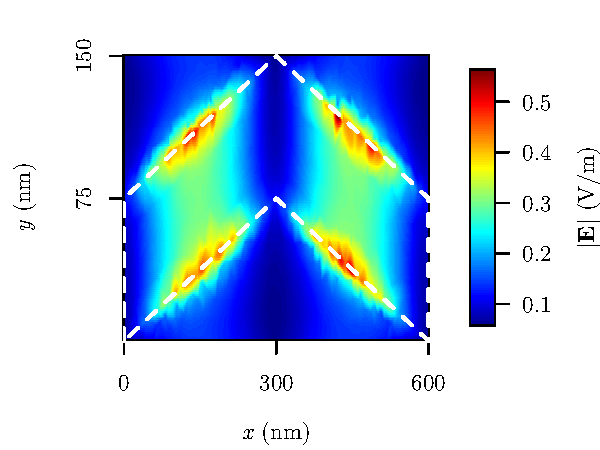
\includegraphics[width=0.49\linewidth]{band-gap-figures/kg-kg-mode1-zEq41nm.pdf}\label{fig:zzbandgapfieldskgkgA}}
		\subfigure[]{\includegraphics[page=2,width=0.49\linewidth]{band-gap-figures/kg-kg-mode1.pdf}\label{fig:zzbandgapfieldskgkgB}}\\	
		\subfigure[]{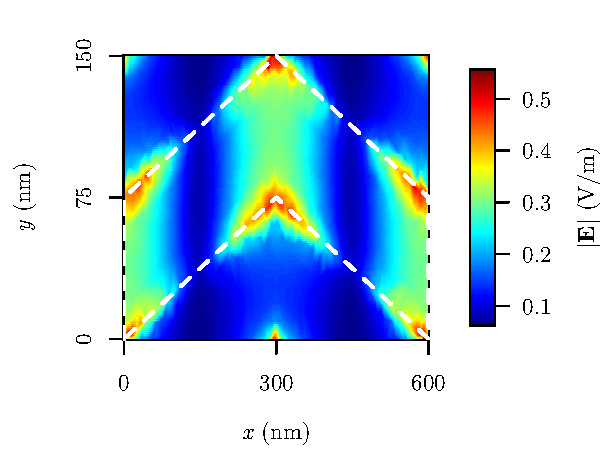
\includegraphics[width=0.49\linewidth]{band-gap-figures/kg-kg-mode2-zEq41nm.pdf}\label{fig:zzbandgapfieldskgkgC}}
		\subfigure[]{\includegraphics[page=2,width=0.49\linewidth]{band-gap-figures/kg-kg-mode2.pdf}\label{fig:zzbandgapfieldskgkgD}}		
	\end{center}	
\caption[The magnitude of electric field for the SPP standing waves at $k_x=0$.]{The magnitude of electric field for the SPP standing waves at $k_x=0$. (a-b) The high-energy solution for (a) the $xy$ plane at $z=41\:\nano\metre$ and (b) the $xz$ plane, for $y=75\:\nano\metre$. (c-d) The low-energy solution for (c) the $xy$ plane at $z=41\:\nano\metre$ and (d) the $xz$ plane, for $y=75\:\nano\metre.$ \label{fig:zzbandgapfieldskgkg}}
\end{figure}

The grating is modelled with the following parameters: $\lambda_{gx}=600\:\nano\metre, \lambda_{gy}=150\:\nano\metre, d=40\:\nano\metre$, with a mark-to-space ratio of 1 and a frequency-dependent silver dielectric function \cite{Nash1996}. We may identify if these standing waves differ in energy, and which of these two is higher in energy relative to the other, by the field decay length into the two media. The higher-energy solution, having been shifted higher in frequency and therefore towards the diffracted light line, will be more photon-like than the lower energy solution, its fields extending further into the dielectric than the low-energy solution. The lower-energy solution will have been shifted lower in frequency, away from the light line and so will be more plasmon-like, constrained closer to the surface. These deductions can be applied in the comparison between the fields of the high energy standing wave in figure \ref{fig:zzbandgapfieldskgkgB} and the lower energy standing wave in figure \ref{fig:zzbandgapfieldskgkgD}. Subfigures \ref{fig:zzbandgapfieldskgkgA} and \ref{fig:zzbandgapfieldskgkgC} show the magnitude of electric field for an arbitrary phase in a plane placed $1\:\nano\metre$ above the zigzag surface at $z=41 \:\nano\metre$. The two field distributions have the expected period of $\lambda_{gx}$. The higher-energy standing wave (figure \ref{fig:zzbandgapfieldskgkgA}) has the field maxima along the edges of the zigzag grooves, while the lower energy standing wave has the field hotspots on the zigzag apexes. It is this energy difference between the two possible standing waves which leads to the plasmonic band-gap.   

Analogous to the case of surface relief gratings, whereby the charge sits at the maxima or minima of the grooves (outlined in the background theory chapter \ref{c:backgroundtheory}), we expect the dependence of this band-gap size to vary as some function of zigzag (in the surface plane) amplitude. 

\begin{figure}
	\begin{center}
	\subfigure[]{
		\begin{minipage}{0.4\linewidth}
		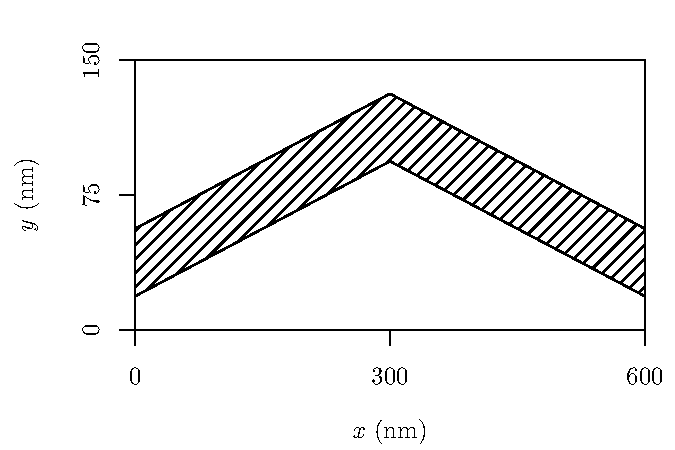
\includegraphics[width=\linewidth]{./band-gap-figures/figure-symmetric-unitcell}	\\
			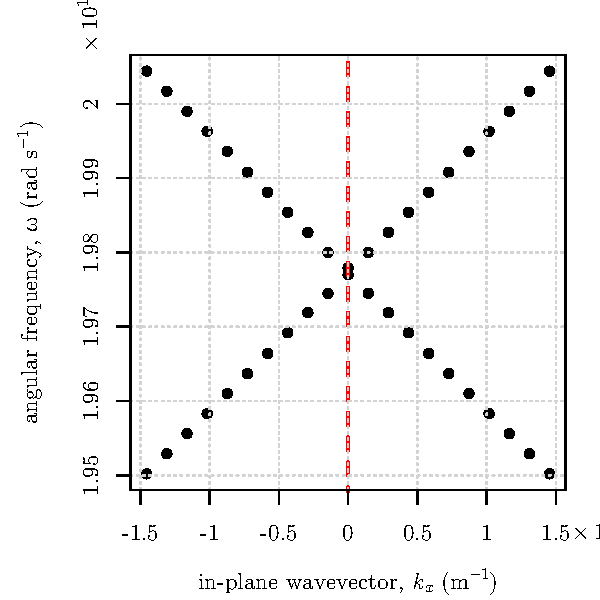
\includegraphics[width=\linewidth]{./band-gap-figures/figure-kgkgbandgap-0offset-dispersion.pdf}
		\end{minipage}
		}
		\subfigure[]{
				\begin{minipage}{0.4\linewidth}
		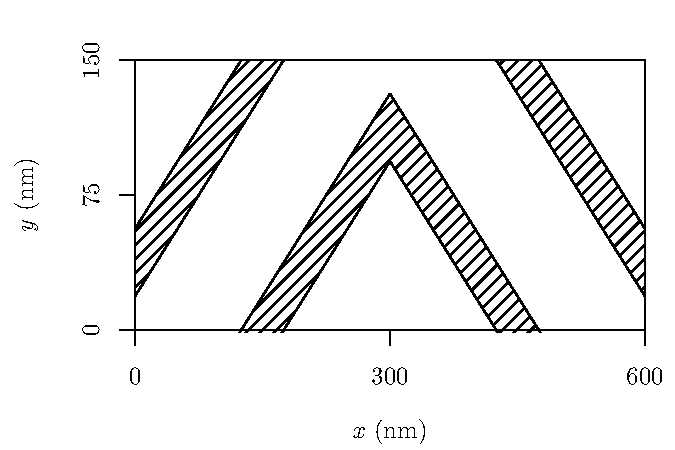
\includegraphics[width=\linewidth]{./band-gap-figures/figure-symmetric-highamp-unitcell}	\\
			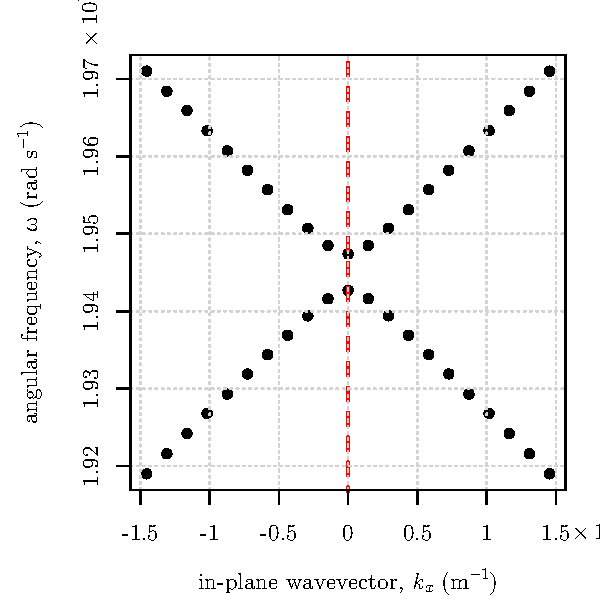
\includegraphics[width=\linewidth]{./band-gap-figures/figure-kgkgbandgap-150yoffset-dispersion.pdf}
		\end{minipage}
		}
	\end{center}
	\caption[Manipulation of the band-gap observed at $k_x=0$ through the increasing of zigzag amplitude.]{Manipulation of the band-gap observed at $k_x=0$ through the increasing of zigzag amplitude.  The unit cell and corresponding SPP dispersion around the intersection of the $+1\mathbf{k}_{gx}$ and $-1\mathbf{k}_{gx}$ scattered SPPs are shown for (a) The zigzag grating presented in this chapter and (b) a theoretical zigzag with a larger zigzag amplitude.  \label{fig:0kx-bandgap-amplitude-dependence}}
\end{figure}

An eigenmode solution is found for two possible unit-cells using FEM modelling, the results of which are shown in figure \ref{fig:0kx-bandgap-amplitude-dependence}.
The parameters for this model used the unit cells shown, with depths of 40 nm, silver parameters from literature \cite{Nash1996} and with the global environment refractive index $n=1.518$. The large-amplitude zig-zag was produced by shifting the central apex in the $y$ direction by 150 nm. This causes multiple zigzags to overlap in a single unit cell, in order to maintain the sub-wavelength period of $\lambda_{gy}=150\:\nano\metre$. It is clearly shown that with an increase of zigzag amplitude, a band-gap is opened at $k_x=0$. This gap is small, as the SPPs must still rely on multiple scattering processes to diffract and interact. This is the first example in this thesis of using the zigzag structure and symmetry to manipulate the band structure of the SPPs, a topic which will be examined further in chapter \ref{c:azigzag}.

\subsection{Band-Gaps at the First Brillouin Zone Boundary}

\begin{figure}
	\begin{center}
	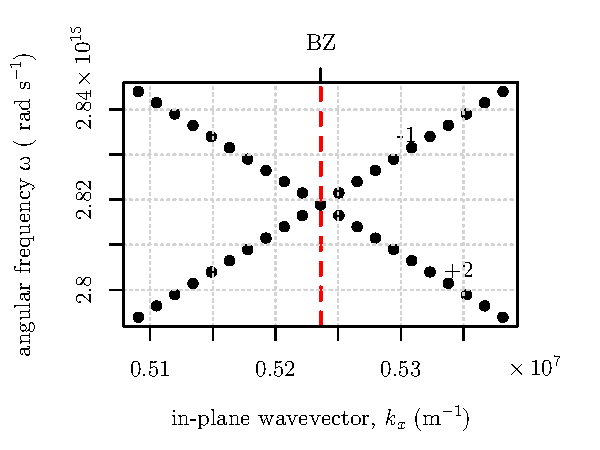
\includegraphics[]{band-gap-figures/2kg-kg-dispersion.pdf}
	\end{center}	
\caption[Modelled SPP dispersion around the intersection point of the $-1\mathbf{k}_{gx}$ and $+2\mathbf{k}_{gx}$ scattered SPPs meeting at the first BZ boundary.]{Modelled SPP dispersion around the intersection point of the $-1\mathbf{k}_{gx}$ and $+2\mathbf{k}_{gx}$ scattered SPPs meeting at the first BZ boundary (red dashed line). \label{fig:zzeigen1stBZ}}
\end{figure}

Normally at Brillouin zone (BZ) boundaries, diffractive coupling results in two counter propagating SPPs, which establish a standing wave \cite{Barnes1996}. The two standing wave solutions correspond to different field distributions with respect to the grating profile, and between these two energy solutions no surface modes propagate: a SPP band-gap forms. However, the experimentally mapped dispersion shown in figures \ref{fig:TEdiseprsionInAir} and \ref{fig:shallowzz-dispersion-expt}, and also the predictions from FEM modelling (figures \ref{fig:TEdiseprsionInAir} and \ref{fig:shallowzz-dispersion-theory}) shows no measurable SPP band-gaps at the first BZ boundaries for this zigzag grating. 

There are two considerations to be made here to determine the possibility of a band-gap between the $-\mathbf{k}_{gx}$ and $+2\mathbf{k}_{gx}$ scattered SPPs: (1) is there a sufficient scattering amplitude present for these modes to Bragg scatter and interact with one another?, and (2) how do the possible standing wave states differ in energy to produce a frequency band of disallowed SPP propagation, if at all? 

Firstly, for the $-\mathbf{k}_{gx}$ and $+2\mathbf{k}_{gx}$ SPPs modes to scatter and interact strongly, they require a total momentum of $3\mathbf{k}_{gx}$. If the grating were to contain a $3\mathbf{k}_{gx}$ component in it's surface profile, this would be a simple direct-scattering event and a strong interaction can occur. Since we observe the $3\mathbf{k}_{gx}$ scattered SPP in the reflectivity mapped in figure \ref{fig:shallowzz-dispersion-expt} (interacting with zero-order light), we can safely assume that the grating provides a strong $3\mathbf{k}_{gx}$ scattering mechanism. However, despite the ability for the grating to scatter SPP modes with a reasonable $3\mathbf{k}_{gx}$ component, there is still no observable band-gap between the $-\mathbf{k}_{gx}$ and $+2\mathbf{k}_{gx}$ at the first BZ boundary. A numerical model of these modes crossing at the BZ is shown in figure \ref{fig:zzeigen1stBZ}. The numerical model is used to extract the possible eigenmodes of the SPPs at the 1st BZ boundary, with modelling parameters of $\lambda_{gx}=600\:\nano\metre, \lambda_{gy}=150\: \nano\metre , d=40\:\nano\metre ,$ a mark-to-space ratio of 1 and $\varepsilon(\omega)$ from literature \cite{Nash1996}. No band-gap is observed, to within the accuracy of the numerical model.

The lack of band-gap at the first BZ boundary is explained considering the allowed standing-wave symmetries on a zigzag grating. Generally, the in-plane wavevector of a standing SPP wave is half that of the total Bragg vector by which the two counter propagating SPPs have been scattered. For the $-\mathbf{k}_{gx}$ and $+2\mathbf{k}_{gx}$ scattered SPPs, crossing at the first BZ boundary, the SPP wavevector is $3\mathbf{k}_{gx}/2$. Through symmetry, there are two possible solutions for this standing wave on a zigzag grating, with the areas of high field of one solution shifted spatially by $\lambda_{gx}/4$ with respect to the other solution. These two solutions are drawn in figure \ref{fig:zzbandgapcartoon}, illustrating the node and anti-node positions of a standing wave along the zigzag. 
\begin{figure}
\begin{center}
\subfigure[]{% Created by tikzDevice version 0.6.2-92-0ad2792 on 2012-12-18 15:38:44
% !TEX encoding = UTF-8 Unicode
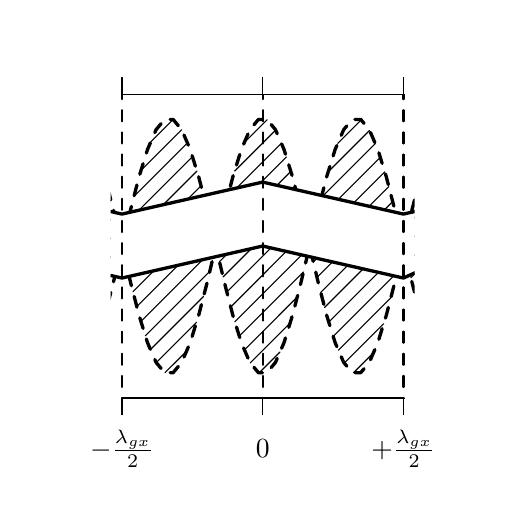
\begin{tikzpicture}[x=1pt,y=1pt]
\definecolor[named]{fillColor}{rgb}{1.00,1.00,1.00}
\path[use as bounding box,fill=fillColor,fill opacity=0.00] (0,0) rectangle (169.83,169.83);
\begin{scope}
\path[clip] ( 30.00, 36.00) rectangle (139.83,145.83);
\definecolor[named]{drawColor}{rgb}{0.00,0.00,0.00}

\path[draw=drawColor,line width= 1.2pt,dash pattern=on 4pt off 4pt ,line join=round,line cap=round] (  0.00, 91.63) --
	(  0.17, 90.92) --
	(  3.25, 77.89) --
	(  6.33, 65.93) --
	(  9.41, 55.98) --
	( 12.50, 48.87) --
	( 15.58, 45.16) --
	( 18.66, 45.16) --
	( 21.74, 48.87) --
	( 24.82, 55.98) --
	( 27.90, 65.93) --
	( 30.99, 77.89) --
	( 34.07, 90.92) --
	( 37.15,103.94) --
	( 40.23,115.91) --
	( 43.31,125.85) --
	( 46.40,132.97) --
	( 49.48,136.67) --
	( 52.56,136.67) --
	( 55.64,132.97) --
	( 58.72,125.85) --
	( 61.80,115.91) --
	( 64.89,103.94) --
	( 67.97, 90.92) --
	( 71.05, 77.89) --
	( 74.13, 65.93) --
	( 77.21, 55.98) --
	( 80.29, 48.87) --
	( 83.38, 45.16) --
	( 86.46, 45.16) --
	( 89.54, 48.87) --
	( 92.62, 55.98) --
	( 95.70, 65.93) --
	( 98.79, 77.89) --
	(101.87, 90.92) --
	(104.95,103.94) --
	(108.03,115.91) --
	(111.11,125.85) --
	(114.19,132.97) --
	(117.28,136.67) --
	(120.36,136.67) --
	(123.44,132.97) --
	(126.52,125.85) --
	(129.60,115.91) --
	(132.68,103.94) --
	(135.77, 90.92) --
	(138.85, 77.89) --
	(141.93, 65.93) --
	(145.01, 55.98) --
	(148.09, 48.87) --
	(151.18, 45.16) --
	(154.26, 45.16) --
	(157.34, 48.87) --
	(160.42, 55.98) --
	(163.50, 65.93) --
	(166.58, 77.89) --
	(169.67, 90.92) --
	(169.83, 91.63);
\end{scope}
\begin{scope}
\path[clip] ( 30.00, 36.00) rectangle (139.83,145.83);
\definecolor[named]{drawColor}{rgb}{0.00,0.00,0.00}

\path[draw=drawColor,line width= 1.2pt,dash pattern=on 4pt off 4pt ,line join=round,line cap=round] (  0.00, 90.21) --
	(  0.17, 90.92) --
	(  3.25,103.94) --
	(  6.33,115.91) --
	(  9.41,125.85) --
	( 12.50,132.97) --
	( 15.58,136.67) --
	( 18.66,136.67) --
	( 21.74,132.97) --
	( 24.82,125.85) --
	( 27.90,115.91) --
	( 30.99,103.94) --
	( 34.07, 90.92) --
	( 37.15, 77.89) --
	( 40.23, 65.93) --
	( 43.31, 55.98) --
	( 46.40, 48.87) --
	( 49.48, 45.16) --
	( 52.56, 45.16) --
	( 55.64, 48.87) --
	( 58.72, 55.98) --
	( 61.80, 65.93) --
	( 64.89, 77.89) --
	( 67.97, 90.92) --
	( 71.05,103.94) --
	( 74.13,115.91) --
	( 77.21,125.85) --
	( 80.29,132.97) --
	( 83.38,136.67) --
	( 86.46,136.67) --
	( 89.54,132.97) --
	( 92.62,125.85) --
	( 95.70,115.91) --
	( 98.79,103.94) --
	(101.87, 90.92) --
	(104.95, 77.89) --
	(108.03, 65.93) --
	(111.11, 55.98) --
	(114.19, 48.87) --
	(117.28, 45.16) --
	(120.36, 45.16) --
	(123.44, 48.87) --
	(126.52, 55.98) --
	(129.60, 65.93) --
	(132.68, 77.89) --
	(135.77, 90.92) --
	(138.85,103.94) --
	(141.93,115.91) --
	(145.01,125.85) --
	(148.09,132.97) --
	(151.18,136.67) --
	(154.26,136.67) --
	(157.34,132.97) --
	(160.42,125.85) --
	(163.50,115.91) --
	(166.58,103.94) --
	(169.67, 90.92) --
	(169.83, 90.21);

\path[draw=drawColor,line width= 0.4pt,line join=round,line cap=round] ( 10.74,128.91) -- ( 18.50,136.67);

\path[draw=drawColor,line width= 0.4pt,line join=round,line cap=round] (  7.13,118.49) -- ( 21.68,133.04);

\path[draw=drawColor,line width= 0.4pt,line join=round,line cap=round] (  4.59,109.13) -- ( 23.76,128.31);

\path[draw=drawColor,line width= 0.4pt,line join=round,line cap=round] (  2.33,100.06) -- ( 25.60,123.33);

\path[draw=drawColor,line width= 0.4pt,line join=round,line cap=round] (  0.00, 90.92) -- (  0.14, 91.05);

\path[draw=drawColor,line width= 0.4pt,line join=round,line cap=round] (  0.22, 91.14) -- ( 27.22,118.13);

\path[draw=drawColor,line width= 0.4pt,line join=round,line cap=round] (  1.44, 85.54) -- (  6.81, 90.92);

\path[draw=drawColor,line width= 0.4pt,line join=round,line cap=round] (  6.81, 90.92) -- ( 28.70,112.81);

\path[draw=drawColor,line width= 0.4pt,line join=round,line cap=round] ( 44.51,128.61) -- ( 52.56,136.67);

\path[draw=drawColor,line width= 0.4pt,line join=round,line cap=round] (  2.74, 80.03) -- ( 13.63, 90.92);

\path[draw=drawColor,line width= 0.4pt,line join=round,line cap=round] ( 13.63, 90.92) -- ( 30.10,107.39);

\path[draw=drawColor,line width= 0.4pt,line join=round,line cap=round] ( 40.96,118.25) -- ( 55.65,132.94);

\path[draw=drawColor,line width= 0.4pt,line join=round,line cap=round] (  4.10, 74.58) -- ( 20.44, 90.92);

\path[draw=drawColor,line width= 0.4pt,line join=round,line cap=round] ( 20.44, 90.92) -- ( 31.46,101.94);

\path[draw=drawColor,line width= 0.4pt,line join=round,line cap=round] ( 38.43,108.90) -- ( 57.71,128.19);

\path[draw=drawColor,line width= 0.4pt,line join=round,line cap=round] (  5.50, 69.16) -- ( 27.25, 90.92);

\path[draw=drawColor,line width= 0.4pt,line join=round,line cap=round] ( 27.25, 90.92) -- ( 32.76, 96.43);

\path[draw=drawColor,line width= 0.4pt,line join=round,line cap=round] ( 36.18, 99.84) -- ( 59.54,123.21);

\path[draw=drawColor,line width= 0.4pt,line join=round,line cap=round] (  6.98, 63.83) -- ( 34.07, 90.92);

\path[draw=drawColor,line width= 0.4pt,line join=round,line cap=round] ( 34.07, 90.92) -- ( 34.07, 90.92);

\path[draw=drawColor,line width= 0.4pt,line join=round,line cap=round] ( 34.07, 90.92) -- ( 61.15,118.00);

\path[draw=drawColor,line width= 0.4pt,line join=round,line cap=round] (  8.59, 58.63) -- ( 31.96, 81.99);

\path[draw=drawColor,line width= 0.4pt,line join=round,line cap=round] ( 35.37, 85.41) -- ( 40.88, 90.92);

\path[draw=drawColor,line width= 0.4pt,line join=round,line cap=round] ( 40.88, 90.92) -- ( 62.64,112.67);

\path[draw=drawColor,line width= 0.4pt,line join=round,line cap=round] ( 78.28,128.32) -- ( 86.54,136.58);

\path[draw=drawColor,line width= 0.4pt,line join=round,line cap=round] ( 10.43, 53.65) -- ( 29.71, 72.93);

\path[draw=drawColor,line width= 0.4pt,line join=round,line cap=round] ( 36.68, 79.90) -- ( 47.70, 90.92);

\path[draw=drawColor,line width= 0.4pt,line join=round,line cap=round] ( 47.70, 90.92) -- ( 64.03,107.25);

\path[draw=drawColor,line width= 0.4pt,line join=round,line cap=round] ( 74.78,118.00) -- ( 89.60,132.82);

\path[draw=drawColor,line width= 0.4pt,line join=round,line cap=round] ( 12.48, 48.89) -- ( 27.18, 63.59);

\path[draw=drawColor,line width= 0.4pt,line join=round,line cap=round] ( 38.04, 74.45) -- ( 54.51, 90.92);

\path[draw=drawColor,line width= 0.4pt,line join=round,line cap=round] ( 54.51, 90.92) -- ( 65.39,101.80);

\path[draw=drawColor,line width= 0.4pt,line join=round,line cap=round] ( 72.27,108.68) -- ( 91.66,128.07);

\path[draw=drawColor,line width= 0.4pt,line join=round,line cap=round] ( 15.57, 45.17) -- ( 23.63, 53.22);

\path[draw=drawColor,line width= 0.4pt,line join=round,line cap=round] ( 39.43, 69.03) -- ( 61.32, 90.92);

\path[draw=drawColor,line width= 0.4pt,line join=round,line cap=round] ( 61.32, 90.92) -- ( 66.70, 96.29);

\path[draw=drawColor,line width= 0.4pt,line join=round,line cap=round] ( 70.03, 99.62) -- ( 93.48,123.08);

\path[draw=drawColor,line width= 0.4pt,line join=round,line cap=round] ( 40.92, 63.70) -- ( 67.92, 90.70);

\path[draw=drawColor,line width= 0.4pt,line join=round,line cap=round] ( 68.00, 90.78) -- ( 68.14, 90.92);

\path[draw=drawColor,line width= 0.4pt,line join=round,line cap=round] ( 68.14, 90.92) -- ( 95.09,117.88);

\path[draw=drawColor,line width= 0.4pt,line join=round,line cap=round] ( 42.53, 58.50) -- ( 65.80, 81.77);

\path[draw=drawColor,line width= 0.4pt,line join=round,line cap=round] ( 69.30, 85.27) -- ( 74.95, 90.92);

\path[draw=drawColor,line width= 0.4pt,line join=round,line cap=round] ( 74.95, 90.92) -- ( 96.57,112.54);

\path[draw=drawColor,line width= 0.4pt,line join=round,line cap=round] (112.05,128.02) -- (120.52,136.48);

\path[draw=drawColor,line width= 0.4pt,line join=round,line cap=round] ( 44.38, 53.53) -- ( 63.55, 72.70);

\path[draw=drawColor,line width= 0.4pt,line join=round,line cap=round] ( 70.61, 79.76) -- ( 81.76, 90.92);

\path[draw=drawColor,line width= 0.4pt,line join=round,line cap=round] ( 81.76, 90.92) -- ( 97.97,107.12);

\path[draw=drawColor,line width= 0.4pt,line join=round,line cap=round] (108.60,117.76) -- (123.55,132.71);

\path[draw=drawColor,line width= 0.4pt,line join=round,line cap=round] ( 46.46, 48.80) -- ( 61.00, 63.34);

\path[draw=drawColor,line width= 0.4pt,line join=round,line cap=round] ( 71.97, 74.31) -- ( 88.58, 90.92);

\path[draw=drawColor,line width= 0.4pt,line join=round,line cap=round] ( 88.58, 90.92) -- ( 99.32,101.66);

\path[draw=drawColor,line width= 0.4pt,line join=round,line cap=round] (106.11,108.45) -- (125.61,127.95);

\path[draw=drawColor,line width= 0.4pt,line join=round,line cap=round] ( 49.63, 45.16) -- ( 57.40, 52.92);

\path[draw=drawColor,line width= 0.4pt,line join=round,line cap=round] ( 73.37, 68.89) -- ( 95.39, 90.92);

\path[draw=drawColor,line width= 0.4pt,line join=round,line cap=round] ( 95.39, 90.92) -- (100.63, 96.15);

\path[draw=drawColor,line width= 0.4pt,line join=round,line cap=round] (103.87, 99.40) -- (127.42,122.95);

\path[draw=drawColor,line width= 0.4pt,line join=round,line cap=round] ( 74.86, 63.57) -- (101.76, 90.47);

\path[draw=drawColor,line width= 0.4pt,line join=round,line cap=round] (101.93, 90.64) -- (102.20, 90.92);

\path[draw=drawColor,line width= 0.4pt,line join=round,line cap=round] (102.20, 90.92) -- (129.03,117.75);

\path[draw=drawColor,line width= 0.4pt,line join=round,line cap=round] ( 76.47, 58.37) -- ( 99.65, 81.55);

\path[draw=drawColor,line width= 0.4pt,line join=round,line cap=round] (103.24, 85.13) -- (109.02, 90.92);

\path[draw=drawColor,line width= 0.4pt,line join=round,line cap=round] (109.02, 90.92) -- (130.51,112.40);

\path[draw=drawColor,line width= 0.4pt,line join=round,line cap=round] (145.82,127.72) -- (154.49,136.39);

\path[draw=drawColor,line width= 0.4pt,line join=round,line cap=round] ( 78.33, 53.41) -- ( 97.39, 72.48);

\path[draw=drawColor,line width= 0.4pt,line join=round,line cap=round] (104.54, 79.62) -- (115.83, 90.92);

\path[draw=drawColor,line width= 0.4pt,line join=round,line cap=round] (115.83, 90.92) -- (131.90,106.99);

\path[draw=drawColor,line width= 0.4pt,line join=round,line cap=round] (142.43,117.51) -- (157.50,132.59);

\path[draw=drawColor,line width= 0.4pt,line join=round,line cap=round] ( 80.43, 48.70) -- ( 94.83, 63.10);

\path[draw=drawColor,line width= 0.4pt,line join=round,line cap=round] (105.91, 74.18) -- (122.65, 90.92);

\path[draw=drawColor,line width= 0.4pt,line join=round,line cap=round] (122.65, 90.92) -- (133.26,101.53);

\path[draw=drawColor,line width= 0.4pt,line join=round,line cap=round] (139.95,108.22) -- (159.56,127.83);

\path[draw=drawColor,line width= 0.4pt,line join=round,line cap=round] ( 83.70, 45.16) -- ( 91.17, 52.63);

\path[draw=drawColor,line width= 0.4pt,line join=round,line cap=round] (107.30, 68.76) -- (129.46, 90.92);

\path[draw=drawColor,line width= 0.4pt,line join=round,line cap=round] (129.46, 90.92) -- (134.56, 96.02);

\path[draw=drawColor,line width= 0.4pt,line join=round,line cap=round] (137.72, 99.18) -- (161.36,122.82);

\path[draw=drawColor,line width= 0.4pt,line join=round,line cap=round] (108.80, 63.44) -- (135.61, 90.25);

\path[draw=drawColor,line width= 0.4pt,line join=round,line cap=round] (135.86, 90.51) -- (136.27, 90.92);

\path[draw=drawColor,line width= 0.4pt,line join=round,line cap=round] (136.27, 90.92) -- (162.97,117.62);

\path[draw=drawColor,line width= 0.4pt,line join=round,line cap=round] (110.41, 58.24) -- (133.50, 81.33);

\path[draw=drawColor,line width= 0.4pt,line join=round,line cap=round] (137.17, 85.00) -- (143.09, 90.92);

\path[draw=drawColor,line width= 0.4pt,line join=round,line cap=round] (143.09, 90.92) -- (164.44,112.27);

\path[draw=drawColor,line width= 0.4pt,line join=round,line cap=round] (112.28, 53.29) -- (131.23, 72.25);

\path[draw=drawColor,line width= 0.4pt,line join=round,line cap=round] (138.47, 79.49) -- (149.90, 90.92);

\path[draw=drawColor,line width= 0.4pt,line join=round,line cap=round] (149.90, 90.92) -- (165.83,106.85);

\path[draw=drawColor,line width= 0.4pt,line join=round,line cap=round] (114.41, 48.61) -- (128.65, 62.85);

\path[draw=drawColor,line width= 0.4pt,line join=round,line cap=round] (139.84, 74.04) -- (156.71, 90.92);

\path[draw=drawColor,line width= 0.4pt,line join=round,line cap=round] (156.71, 90.92) -- (167.19,101.39);

\path[draw=drawColor,line width= 0.4pt,line join=round,line cap=round] (117.77, 45.16) -- (124.94, 52.33);

\path[draw=drawColor,line width= 0.4pt,line join=round,line cap=round] (141.24, 68.62) -- (163.53, 90.92);

\path[draw=drawColor,line width= 0.4pt,line join=round,line cap=round] (163.53, 90.92) -- (168.49, 95.88);

\path[draw=drawColor,line width= 0.4pt,line join=round,line cap=round] (142.74, 63.31) -- (169.46, 90.03);

\path[draw=drawColor,line width= 0.4pt,line join=round,line cap=round] (169.80, 90.37) -- (169.83, 90.41);

\path[draw=drawColor,line width= 0.4pt,line join=round,line cap=round] (144.35, 58.11) -- (167.34, 81.11);

\path[draw=drawColor,line width= 0.4pt,line join=round,line cap=round] (146.23, 53.18) -- (165.07, 72.02);

\path[draw=drawColor,line width= 0.4pt,line join=round,line cap=round] (148.38, 48.52) -- (162.47, 62.61);

\path[draw=drawColor,line width= 0.4pt,line join=round,line cap=round] (151.84, 45.16) -- (158.71, 52.03);

\path[] (  0.00, 91.63) --
	(  0.17, 90.92) --
	(  3.25, 77.89) --
	(  6.33, 65.93) --
	(  9.41, 55.98) --
	( 12.50, 48.87) --
	( 15.58, 45.16) --
	( 18.66, 45.16) --
	( 21.74, 48.87) --
	( 24.82, 55.98) --
	( 27.90, 65.93) --
	( 30.99, 77.89) --
	( 34.07, 90.92) --
	( 37.15,103.94) --
	( 40.23,115.91) --
	( 43.31,125.85) --
	( 46.40,132.97) --
	( 49.48,136.67) --
	( 52.56,136.67) --
	( 55.64,132.97) --
	( 58.72,125.85) --
	( 61.80,115.91) --
	( 64.89,103.94) --
	( 67.97, 90.92) --
	( 71.05, 77.89) --
	( 74.13, 65.93) --
	( 77.21, 55.98) --
	( 80.29, 48.87) --
	( 83.38, 45.16) --
	( 86.46, 45.16) --
	( 89.54, 48.87) --
	( 92.62, 55.98) --
	( 95.70, 65.93) --
	( 98.79, 77.89) --
	(101.87, 90.92) --
	(104.95,103.94) --
	(108.03,115.91) --
	(111.11,125.85) --
	(114.19,132.97) --
	(117.28,136.67) --
	(120.36,136.67) --
	(123.44,132.97) --
	(126.52,125.85) --
	(129.60,115.91) --
	(132.68,103.94) --
	(135.77, 90.92) --
	(138.85, 77.89) --
	(141.93, 65.93) --
	(145.01, 55.98) --
	(148.09, 48.87) --
	(151.18, 45.16) --
	(154.26, 45.16) --
	(157.34, 48.87) --
	(160.42, 55.98) --
	(163.50, 65.93) --
	(166.58, 77.89) --
	(169.67, 90.92) --
	(169.83, 91.63);

\path[] (169.83, 90.92) --
	(  0.00, 90.92);

\path[] (  0.00, 90.21) --
	(  0.17, 90.92) --
	(  3.25,103.94) --
	(  6.33,115.91) --
	(  9.41,125.85) --
	( 12.50,132.97) --
	( 15.58,136.67) --
	( 18.66,136.67) --
	( 21.74,132.97) --
	( 24.82,125.85) --
	( 27.90,115.91) --
	( 30.99,103.94) --
	( 34.07, 90.92) --
	( 37.15, 77.89) --
	( 40.23, 65.93) --
	( 43.31, 55.98) --
	( 46.40, 48.87) --
	( 49.48, 45.16) --
	( 52.56, 45.16) --
	( 55.64, 48.87) --
	( 58.72, 55.98) --
	( 61.80, 65.93) --
	( 64.89, 77.89) --
	( 67.97, 90.92) --
	( 71.05,103.94) --
	( 74.13,115.91) --
	( 77.21,125.85) --
	( 80.29,132.97) --
	( 83.38,136.67) --
	( 86.46,136.67) --
	( 89.54,132.97) --
	( 92.62,125.85) --
	( 95.70,115.91) --
	( 98.79,103.94) --
	(101.87, 90.92) --
	(104.95, 77.89) --
	(108.03, 65.93) --
	(111.11, 55.98) --
	(114.19, 48.87) --
	(117.28, 45.16) --
	(120.36, 45.16) --
	(123.44, 48.87) --
	(126.52, 55.98) --
	(129.60, 65.93) --
	(132.68, 77.89) --
	(135.77, 90.92) --
	(138.85,103.94) --
	(141.93,115.91) --
	(145.01,125.85) --
	(148.09,132.97) --
	(151.18,136.67) --
	(154.26,136.67) --
	(157.34,132.97) --
	(160.42,125.85) --
	(163.50,115.91) --
	(166.58,103.94) --
	(169.67, 90.92) --
	(169.83, 90.21);

\path[] (169.83, 90.92) --
	(  0.00, 90.92);
\definecolor[named]{fillColor}{rgb}{1.00,1.00,1.00}

\path[draw=drawColor,line width= 1.2pt,line join=round,line cap=round,fill=fillColor] ( 34.07, 79.36) --
	(  0.00, 87.10) --
	(  0.00,110.22) --
	( 34.07,102.47) --
	( 84.92,114.03) --
	(135.77,102.47) --
	(169.83,110.22) --
	(169.83, 94.85) --
	(135.77, 79.36) --
	( 84.92, 90.92) --
	cycle;
\end{scope}
\begin{scope}
\path[clip] (  0.00,  0.00) rectangle (169.83,169.83);
\definecolor[named]{drawColor}{rgb}{0.00,0.00,0.00}

\path[draw=drawColor,line width= 0.4pt,line join=round,line cap=round] ( 34.07, 36.00) -- (135.77, 36.00);

\path[draw=drawColor,line width= 0.4pt,line join=round,line cap=round] ( 34.07, 36.00) -- ( 34.07, 30.00);

\path[draw=drawColor,line width= 0.4pt,line join=round,line cap=round] ( 84.92, 36.00) -- ( 84.92, 30.00);

\path[draw=drawColor,line width= 0.4pt,line join=round,line cap=round] (135.77, 36.00) -- (135.77, 30.00);

\node[text=drawColor,anchor=base,inner sep=0pt, outer sep=0pt, scale=  1.00] at ( 34.07, 14.40) {$-\frac{\lambda_{gx}}{2}$};

\node[text=drawColor,anchor=base,inner sep=0pt, outer sep=0pt, scale=  1.00] at ( 84.92, 14.40) {$0$};

\node[text=drawColor,anchor=base,inner sep=0pt, outer sep=0pt, scale=  1.00] at (135.77, 14.40) {$+\frac{\lambda_{gx}}{2}$};

\path[draw=drawColor,line width= 0.4pt,line join=round,line cap=round] ( 34.07,145.83) -- (135.77,145.83);

\path[draw=drawColor,line width= 0.4pt,line join=round,line cap=round] ( 34.07,145.83) -- ( 34.07,151.83);

\path[draw=drawColor,line width= 0.4pt,line join=round,line cap=round] ( 84.92,145.83) -- ( 84.92,151.83);

\path[draw=drawColor,line width= 0.4pt,line join=round,line cap=round] (135.77,145.83) -- (135.77,151.83);
\end{scope}
\begin{scope}
\path[clip] ( 30.00, 36.00) rectangle (139.83,145.83);
\definecolor[named]{drawColor}{rgb}{0.00,0.00,0.00}

\path[draw=drawColor,line width= 0.8pt,dash pattern=on 4pt off 4pt ,line join=round,line cap=round] ( 34.07,  0.00) --
	( 34.07,169.83);

\path[draw=drawColor,line width= 0.8pt,dash pattern=on 4pt off 4pt ,line join=round,line cap=round] (135.77,  0.00) --
	(135.77,169.83);

\path[draw=drawColor,line width= 0.8pt,dash pattern=on 4pt off 4pt ,line join=round,line cap=round] ( 84.92,  0.00) --
	( 84.92,169.83);
\end{scope}
\end{tikzpicture}
}
\subfigure[]{% Created by tikzDevice version 0.6.2-92-0ad2792 on 2012-12-18 15:38:44
% !TEX encoding = UTF-8 Unicode
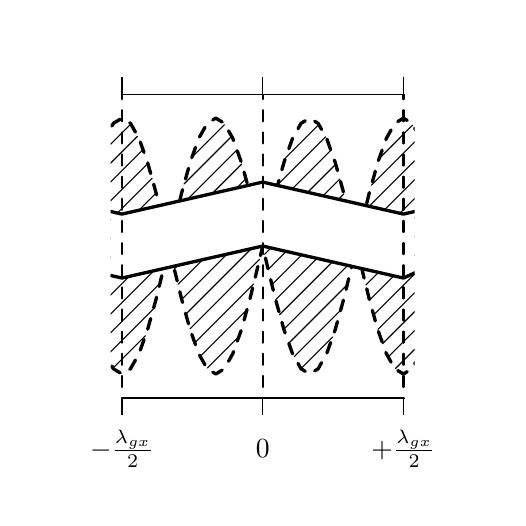
\begin{tikzpicture}[x=1pt,y=1pt]
\definecolor[named]{fillColor}{rgb}{1.00,1.00,1.00}
\path[use as bounding box,fill=fillColor,fill opacity=0.00] (0,0) rectangle (169.83,169.83);
\begin{scope}
\path[clip] ( 30.00, 36.00) rectangle (139.83,145.83);
\definecolor[named]{drawColor}{rgb}{0.00,0.00,0.00}

\path[draw=drawColor,line width= 1.2pt,dash pattern=on 4pt off 4pt ,line join=round,line cap=round] (  0.00, 44.79) --
	(  0.17, 44.69) --
	(  3.25, 46.56) --
	(  6.33, 52.03) --
	(  9.41, 60.65) --
	( 12.50, 71.71) --
	( 15.58, 84.34) --
	( 18.66, 97.50) --
	( 21.74,110.12) --
	( 24.82,121.19) --
	( 27.90,129.81) --
	( 30.99,135.27) --
	( 34.07,137.14) --
	( 37.15,135.27) --
	( 40.23,129.81) --
	( 43.31,121.19) --
	( 46.40,110.12) --
	( 49.48, 97.50) --
	( 52.56, 84.34) --
	( 55.64, 71.71) --
	( 58.72, 60.65) --
	( 61.80, 52.03) --
	( 64.89, 46.56) --
	( 67.97, 44.69) --
	( 71.05, 46.56) --
	( 74.13, 52.03) --
	( 77.21, 60.65) --
	( 80.29, 71.71) --
	( 83.38, 84.34) --
	( 86.46, 97.50) --
	( 89.54,110.12) --
	( 92.62,121.19) --
	( 95.70,129.81) --
	( 98.79,135.27) --
	(101.87,137.14) --
	(104.95,135.27) --
	(108.03,129.81) --
	(111.11,121.19) --
	(114.19,110.12) --
	(117.28, 97.50) --
	(120.36, 84.34) --
	(123.44, 71.71) --
	(126.52, 60.65) --
	(129.60, 52.03) --
	(132.68, 46.56) --
	(135.77, 44.69) --
	(138.85, 46.56) --
	(141.93, 52.03) --
	(145.01, 60.65) --
	(148.09, 71.71) --
	(151.18, 84.34) --
	(154.26, 97.50) --
	(157.34,110.12) --
	(160.42,121.19) --
	(163.50,129.81) --
	(166.58,135.27) --
	(169.67,137.14) --
	(169.83,137.04);
\end{scope}
\begin{scope}
\path[clip] ( 30.00, 36.00) rectangle (139.83,145.83);
\definecolor[named]{drawColor}{rgb}{0.00,0.00,0.00}

\path[draw=drawColor,line width= 1.2pt,dash pattern=on 4pt off 4pt ,line join=round,line cap=round] (  0.00,137.04) --
	(  0.17,137.14) --
	(  3.25,135.27) --
	(  6.33,129.81) --
	(  9.41,121.19) --
	( 12.50,110.12) --
	( 15.58, 97.50) --
	( 18.66, 84.34) --
	( 21.74, 71.71) --
	( 24.82, 60.65) --
	( 27.90, 52.03) --
	( 30.99, 46.56) --
	( 34.07, 44.69) --
	( 37.15, 46.56) --
	( 40.23, 52.03) --
	( 43.31, 60.65) --
	( 46.40, 71.71) --
	( 49.48, 84.34) --
	( 52.56, 97.50) --
	( 55.64,110.12) --
	( 58.72,121.19) --
	( 61.80,129.81) --
	( 64.89,135.27) --
	( 67.97,137.14) --
	( 71.05,135.27) --
	( 74.13,129.81) --
	( 77.21,121.19) --
	( 80.29,110.12) --
	( 83.38, 97.50) --
	( 86.46, 84.34) --
	( 89.54, 71.71) --
	( 92.62, 60.65) --
	( 95.70, 52.03) --
	( 98.79, 46.56) --
	(101.87, 44.69) --
	(104.95, 46.56) --
	(108.03, 52.03) --
	(111.11, 60.65) --
	(114.19, 71.71) --
	(117.28, 84.34) --
	(120.36, 97.50) --
	(123.44,110.12) --
	(126.52,121.19) --
	(129.60,129.81) --
	(132.68,135.27) --
	(135.77,137.14) --
	(138.85,135.27) --
	(141.93,129.81) --
	(145.01,121.19) --
	(148.09,110.12) --
	(151.18, 97.50) --
	(154.26, 84.34) --
	(157.34, 71.71) --
	(160.42, 60.65) --
	(163.50, 52.03) --
	(166.58, 46.56) --
	(169.67, 44.69) --
	(169.83, 44.79);

\path[draw=drawColor,line width= 0.4pt,line join=round,line cap=round] (  0.00,131.80) -- (  3.15,134.95);

\path[draw=drawColor,line width= 0.4pt,line join=round,line cap=round] (  0.00,124.99) -- (  5.76,130.74);

\path[draw=drawColor,line width= 0.4pt,line join=round,line cap=round] (  0.00,118.17) -- (  7.81,125.99);

\path[draw=drawColor,line width= 0.4pt,line join=round,line cap=round] (  0.00,111.36) -- (  9.44,120.80);

\path[draw=drawColor,line width= 0.4pt,line join=round,line cap=round] (  0.00,104.55) -- ( 11.04,115.58);

\path[draw=drawColor,line width= 0.4pt,line join=round,line cap=round] (  0.00, 97.73) -- ( 12.43,110.17);

\path[draw=drawColor,line width= 0.4pt,line join=round,line cap=round] ( 25.57,123.31) -- ( 37.12,134.85);

\path[draw=drawColor,line width= 0.4pt,line join=round,line cap=round] (  0.00, 90.92) -- ( 13.83,104.75);

\path[draw=drawColor,line width= 0.4pt,line join=round,line cap=round] ( 22.69,113.61) -- ( 39.71,130.62);

\path[draw=drawColor,line width= 0.4pt,line join=round,line cap=round] (  0.00, 84.10) -- (  6.81, 90.92);

\path[draw=drawColor,line width= 0.4pt,line join=round,line cap=round] (  6.81, 90.92) -- ( 15.15, 99.25);

\path[draw=drawColor,line width= 0.4pt,line join=round,line cap=round] ( 20.33,104.43) -- ( 41.77,125.87);

\path[draw=drawColor,line width= 0.4pt,line join=round,line cap=round] (  0.00, 77.29) -- ( 13.63, 90.92);

\path[draw=drawColor,line width= 0.4pt,line join=round,line cap=round] ( 13.63, 90.92) -- ( 16.45, 93.74);

\path[draw=drawColor,line width= 0.4pt,line join=round,line cap=round] ( 18.20, 95.49) -- ( 43.38,120.67);

\path[draw=drawColor,line width= 0.4pt,line join=round,line cap=round] (  0.00, 70.48) -- ( 16.09, 86.56);

\path[draw=drawColor,line width= 0.4pt,line join=round,line cap=round] ( 17.75, 88.23) -- ( 20.44, 90.92);

\path[draw=drawColor,line width= 0.4pt,line join=round,line cap=round] ( 20.44, 90.92) -- ( 44.97,115.45);

\path[draw=drawColor,line width= 0.4pt,line join=round,line cap=round] (  0.00, 63.66) -- ( 13.97, 77.63);

\path[draw=drawColor,line width= 0.4pt,line join=round,line cap=round] ( 19.06, 82.72) -- ( 27.25, 90.92);

\path[draw=drawColor,line width= 0.4pt,line join=round,line cap=round] ( 27.25, 90.92) -- ( 46.37,110.03);

\path[draw=drawColor,line width= 0.4pt,line join=round,line cap=round] ( 59.40,123.06) -- ( 71.10,134.76);

\path[draw=drawColor,line width= 0.4pt,line join=round,line cap=round] (  0.00, 56.85) -- ( 11.61, 68.46);

\path[draw=drawColor,line width= 0.4pt,line join=round,line cap=round] ( 20.37, 77.22) -- ( 34.07, 90.92);

\path[draw=drawColor,line width= 0.4pt,line join=round,line cap=round] ( 34.07, 90.92) -- ( 47.76,104.61);

\path[draw=drawColor,line width= 0.4pt,line join=round,line cap=round] ( 56.53,113.38) -- ( 73.66,130.51);

\path[draw=drawColor,line width= 0.4pt,line join=round,line cap=round] (  0.00, 50.04) -- (  8.74, 58.77);

\path[draw=drawColor,line width= 0.4pt,line join=round,line cap=round] ( 21.77, 71.80) -- ( 40.88, 90.92);

\path[draw=drawColor,line width= 0.4pt,line join=round,line cap=round] ( 40.88, 90.92) -- ( 49.08, 99.11);

\path[draw=drawColor,line width= 0.4pt,line join=round,line cap=round] ( 54.17,104.20) -- ( 75.71,125.74);

\path[draw=drawColor,line width= 0.4pt,line join=round,line cap=round] ( 23.16, 66.39) -- ( 47.70, 90.92);

\path[draw=drawColor,line width= 0.4pt,line join=round,line cap=round] ( 47.70, 90.92) -- ( 50.38, 93.60);

\path[draw=drawColor,line width= 0.4pt,line join=round,line cap=round] ( 52.05, 95.27) -- ( 77.32,120.54);

\path[draw=drawColor,line width= 0.4pt,line join=round,line cap=round] ( 24.76, 61.17) -- ( 49.94, 86.34);

\path[draw=drawColor,line width= 0.4pt,line join=round,line cap=round] ( 51.69, 88.09) -- ( 54.51, 90.92);

\path[draw=drawColor,line width= 0.4pt,line join=round,line cap=round] ( 54.51, 90.92) -- ( 78.91,115.31);

\path[draw=drawColor,line width= 0.4pt,line join=round,line cap=round] ( 26.37, 55.97) -- ( 47.81, 77.40);

\path[draw=drawColor,line width= 0.4pt,line join=round,line cap=round] ( 52.99, 82.58) -- ( 61.32, 90.92);

\path[draw=drawColor,line width= 0.4pt,line join=round,line cap=round] ( 61.32, 90.92) -- ( 80.30,109.90);

\path[draw=drawColor,line width= 0.4pt,line join=round,line cap=round] ( 93.22,122.82) -- (105.07,134.67);

\path[draw=drawColor,line width= 0.4pt,line join=round,line cap=round] ( 28.43, 51.21) -- ( 45.45, 68.23);

\path[draw=drawColor,line width= 0.4pt,line join=round,line cap=round] ( 54.31, 77.09) -- ( 68.14, 90.92);

\path[draw=drawColor,line width= 0.4pt,line join=round,line cap=round] ( 68.14, 90.92) -- ( 81.70,104.48);

\path[draw=drawColor,line width= 0.4pt,line join=round,line cap=round] ( 90.37,113.15) -- (107.61,130.39);

\path[draw=drawColor,line width= 0.4pt,line join=round,line cap=round] ( 31.01, 46.98) -- ( 42.56, 58.53);

\path[draw=drawColor,line width= 0.4pt,line join=round,line cap=round] ( 55.70, 71.67) -- ( 74.95, 90.92);

\path[draw=drawColor,line width= 0.4pt,line join=round,line cap=round] ( 74.95, 90.92) -- ( 83.01, 98.98);

\path[draw=drawColor,line width= 0.4pt,line join=round,line cap=round] ( 88.01,103.98) -- (109.65,125.61);

\path[draw=drawColor,line width= 0.4pt,line join=round,line cap=round] ( 57.10, 66.25) -- ( 81.76, 90.92);

\path[draw=drawColor,line width= 0.4pt,line join=round,line cap=round] ( 81.76, 90.92) -- ( 84.31, 93.47);

\path[draw=drawColor,line width= 0.4pt,line join=round,line cap=round] ( 85.89, 95.05) -- (111.26,120.41);

\path[draw=drawColor,line width= 0.4pt,line join=round,line cap=round] ( 58.70, 61.04) -- ( 83.78, 86.12);

\path[draw=drawColor,line width= 0.4pt,line join=round,line cap=round] ( 85.62, 87.96) -- ( 88.58, 90.92);

\path[draw=drawColor,line width= 0.4pt,line join=round,line cap=round] ( 88.58, 90.92) -- (112.84,115.18);

\path[draw=drawColor,line width= 0.4pt,line join=round,line cap=round] (133.69,136.03) -- (134.33,136.67);

\path[draw=drawColor,line width= 0.4pt,line join=round,line cap=round] ( 60.32, 55.85) -- ( 81.65, 77.18);

\path[draw=drawColor,line width= 0.4pt,line join=round,line cap=round] ( 86.92, 82.45) -- ( 95.39, 90.92);

\path[draw=drawColor,line width= 0.4pt,line join=round,line cap=round] ( 95.39, 90.92) -- (114.24,109.76);

\path[draw=drawColor,line width= 0.4pt,line join=round,line cap=round] (127.05,122.57) -- (139.05,134.58);

\path[draw=drawColor,line width= 0.4pt,line join=round,line cap=round] ( 62.38, 51.09) -- ( 79.29, 68.00);

\path[draw=drawColor,line width= 0.4pt,line join=round,line cap=round] ( 88.24, 76.95) -- (102.20, 90.92);

\path[draw=drawColor,line width= 0.4pt,line join=round,line cap=round] (102.20, 90.92) -- (115.63,104.34);

\path[draw=drawColor,line width= 0.4pt,line join=round,line cap=round] (124.21,112.92) -- (141.56,130.27);

\path[draw=drawColor,line width= 0.4pt,line join=round,line cap=round] ( 64.99, 46.89) -- ( 76.39, 58.28);

\path[draw=drawColor,line width= 0.4pt,line join=round,line cap=round] ( 89.64, 71.54) -- (109.02, 90.92);

\path[draw=drawColor,line width= 0.4pt,line join=round,line cap=round] (109.02, 90.92) -- (116.94, 98.84);

\path[draw=drawColor,line width= 0.4pt,line join=round,line cap=round] (121.85,103.75) -- (143.59,125.48);

\path[draw=drawColor,line width= 0.4pt,line join=round,line cap=round] ( 91.03, 66.12) -- (115.83, 90.92);

\path[draw=drawColor,line width= 0.4pt,line join=round,line cap=round] (115.83, 90.92) -- (118.25, 93.33);

\path[draw=drawColor,line width= 0.4pt,line join=round,line cap=round] (119.74, 94.83) -- (145.20,120.28);

\path[draw=drawColor,line width= 0.4pt,line join=round,line cap=round] ( 92.64, 60.91) -- (117.63, 85.90);

\path[draw=drawColor,line width= 0.4pt,line join=round,line cap=round] (119.55, 87.82) -- (122.65, 90.92);

\path[draw=drawColor,line width= 0.4pt,line join=round,line cap=round] (122.65, 90.92) -- (146.77,115.05);

\path[draw=drawColor,line width= 0.4pt,line join=round,line cap=round] (166.76,135.03) -- (168.40,136.67);

\path[draw=drawColor,line width= 0.4pt,line join=round,line cap=round] ( 94.27, 55.73) -- (115.49, 76.95);

\path[draw=drawColor,line width= 0.4pt,line join=round,line cap=round] (120.85, 82.31) -- (129.46, 90.92);

\path[draw=drawColor,line width= 0.4pt,line join=round,line cap=round] (129.46, 90.92) -- (148.17,109.63);

\path[draw=drawColor,line width= 0.4pt,line join=round,line cap=round] (160.87,122.33) -- (169.83,131.29);

\path[draw=drawColor,line width= 0.4pt,line join=round,line cap=round] ( 96.33, 50.98) -- (113.13, 67.77);

\path[draw=drawColor,line width= 0.4pt,line join=round,line cap=round] (122.18, 76.82) -- (136.27, 90.92);

\path[draw=drawColor,line width= 0.4pt,line join=round,line cap=round] (136.27, 90.92) -- (149.57,104.21);

\path[draw=drawColor,line width= 0.4pt,line join=round,line cap=round] (158.05,112.70) -- (169.83,124.48);

\path[draw=drawColor,line width= 0.4pt,line join=round,line cap=round] ( 98.97, 46.80) -- (110.21, 58.04);

\path[draw=drawColor,line width= 0.4pt,line join=round,line cap=round] (123.57, 71.40) -- (143.09, 90.92);

\path[draw=drawColor,line width= 0.4pt,line join=round,line cap=round] (143.09, 90.92) -- (150.87, 98.70);

\path[draw=drawColor,line width= 0.4pt,line join=round,line cap=round] (155.70,103.53) -- (169.83,117.66);

\path[draw=drawColor,line width= 0.4pt,line join=round,line cap=round] (124.97, 65.98) -- (149.90, 90.92);

\path[draw=drawColor,line width= 0.4pt,line join=round,line cap=round] (149.90, 90.92) -- (152.18, 93.19);

\path[draw=drawColor,line width= 0.4pt,line join=round,line cap=round] (153.59, 94.61) -- (169.83,110.85);

\path[draw=drawColor,line width= 0.4pt,line join=round,line cap=round] (126.58, 60.78) -- (151.48, 85.68);

\path[draw=drawColor,line width= 0.4pt,line join=round,line cap=round] (153.48, 87.68) -- (156.71, 90.92);

\path[draw=drawColor,line width= 0.4pt,line join=round,line cap=round] (156.71, 90.92) -- (169.83,104.04);

\path[draw=drawColor,line width= 0.4pt,line join=round,line cap=round] (128.22, 55.61) -- (149.33, 76.72);

\path[draw=drawColor,line width= 0.4pt,line join=round,line cap=round] (154.79, 82.17) -- (163.53, 90.92);

\path[draw=drawColor,line width= 0.4pt,line join=round,line cap=round] (163.53, 90.92) -- (169.83, 97.22);

\path[draw=drawColor,line width= 0.4pt,line join=round,line cap=round] (130.28, 50.86) -- (146.97, 67.55);

\path[draw=drawColor,line width= 0.4pt,line join=round,line cap=round] (156.11, 76.69) -- (169.83, 90.41);

\path[draw=drawColor,line width= 0.4pt,line join=round,line cap=round] (132.94, 46.70) -- (144.03, 57.80);

\path[draw=drawColor,line width= 0.4pt,line join=round,line cap=round] (157.50, 71.27) -- (169.83, 83.60);

\path[draw=drawColor,line width= 0.4pt,line join=round,line cap=round] (158.90, 65.85) -- (169.83, 76.78);

\path[draw=drawColor,line width= 0.4pt,line join=round,line cap=round] (160.51, 60.65) -- (169.83, 69.97);

\path[draw=drawColor,line width= 0.4pt,line join=round,line cap=round] (162.17, 55.49) -- (169.83, 63.16);

\path[draw=drawColor,line width= 0.4pt,line join=round,line cap=round] (164.23, 50.74) -- (169.83, 56.34);

\path[draw=drawColor,line width= 0.4pt,line join=round,line cap=round] (166.92, 46.61) -- (169.83, 49.53);

\path[] (  0.00, 45.16) --
	(  1.71, 45.16) --
	(  4.79, 48.87) --
	(  7.87, 55.98) --
	( 10.95, 65.93) --
	( 14.04, 77.89) --
	( 17.12, 90.92) --
	( 20.20,103.94) --
	( 23.28,115.91) --
	( 26.36,125.85) --
	( 29.45,132.97) --
	( 32.53,136.67) --
	( 35.61,136.67) --
	( 38.69,132.97) --
	( 41.77,125.85) --
	( 44.85,115.91) --
	( 47.94,103.94) --
	( 51.02, 90.92) --
	( 54.10, 77.89) --
	( 57.18, 65.93) --
	( 60.26, 55.98) --
	( 63.34, 48.87) --
	( 66.43, 45.16) --
	( 69.51, 45.16) --
	( 72.59, 48.87) --
	( 75.67, 55.98) --
	( 78.75, 65.93) --
	( 81.84, 77.89) --
	( 84.92, 90.92) --
	( 88.00,103.94) --
	( 91.08,115.91) --
	( 94.16,125.85) --
	( 97.24,132.97) --
	(100.33,136.67) --
	(103.41,136.67) --
	(106.49,132.97) --
	(109.57,125.85) --
	(112.65,115.91) --
	(115.74,103.94) --
	(118.82, 90.92) --
	(121.90, 77.89) --
	(124.98, 65.93) --
	(128.06, 55.98) --
	(131.14, 48.87) --
	(134.23, 45.16) --
	(137.31, 45.16) --
	(140.39, 48.87) --
	(143.47, 55.98) --
	(146.55, 65.93) --
	(149.63, 77.89) --
	(152.72, 90.92) --
	(155.80,103.94) --
	(158.88,115.91) --
	(161.96,125.85) --
	(165.04,132.97) --
	(168.13,136.67) --
	(169.83,136.67);

\path[] (169.83, 90.92) --
	(  0.00, 90.92);

\path[] (  0.00,136.67) --
	(  1.71,136.67) --
	(  4.79,132.97) --
	(  7.87,125.85) --
	( 10.95,115.91) --
	( 14.04,103.94) --
	( 17.12, 90.92) --
	( 20.20, 77.89) --
	( 23.28, 65.93) --
	( 26.36, 55.98) --
	( 29.45, 48.87) --
	( 32.53, 45.16) --
	( 35.61, 45.16) --
	( 38.69, 48.87) --
	( 41.77, 55.98) --
	( 44.85, 65.93) --
	( 47.94, 77.89) --
	( 51.02, 90.92) --
	( 54.10,103.94) --
	( 57.18,115.91) --
	( 60.26,125.85) --
	( 63.34,132.97) --
	( 66.43,136.67) --
	( 69.51,136.67) --
	( 72.59,132.97) --
	( 75.67,125.85) --
	( 78.75,115.91) --
	( 81.84,103.94) --
	( 84.92, 90.92) --
	( 88.00, 77.89) --
	( 91.08, 65.93) --
	( 94.16, 55.98) --
	( 97.24, 48.87) --
	(100.33, 45.16) --
	(103.41, 45.16) --
	(106.49, 48.87) --
	(109.57, 55.98) --
	(112.65, 65.93) --
	(115.74, 77.89) --
	(118.82, 90.92) --
	(121.90,103.94) --
	(124.98,115.91) --
	(128.06,125.85) --
	(131.14,132.97) --
	(134.23,136.67) --
	(137.31,136.67) --
	(140.39,132.97) --
	(143.47,125.85) --
	(146.55,115.91) --
	(149.63,103.94) --
	(152.72, 90.92) --
	(155.80, 77.89) --
	(158.88, 65.93) --
	(161.96, 55.98) --
	(165.04, 48.87) --
	(168.13, 45.16) --
	(169.83, 45.16);

\path[] (169.83, 90.92) --
	(  0.00, 90.92);
\definecolor[named]{fillColor}{rgb}{1.00,1.00,1.00}

\path[draw=drawColor,line width= 1.2pt,line join=round,line cap=round,fill=fillColor] ( 34.07, 79.36) --
	(  0.00, 87.10) --
	(  0.00,110.22) --
	( 34.07,102.47) --
	( 84.92,114.03) --
	(135.77,102.47) --
	(169.83,110.22) --
	(169.83, 94.85) --
	(135.77, 79.36) --
	( 84.92, 90.92) --
	cycle;
\end{scope}
\begin{scope}
\path[clip] (  0.00,  0.00) rectangle (169.83,169.83);
\definecolor[named]{drawColor}{rgb}{0.00,0.00,0.00}

\path[draw=drawColor,line width= 0.4pt,line join=round,line cap=round] ( 34.07, 36.00) -- (135.77, 36.00);

\path[draw=drawColor,line width= 0.4pt,line join=round,line cap=round] ( 34.07, 36.00) -- ( 34.07, 30.00);

\path[draw=drawColor,line width= 0.4pt,line join=round,line cap=round] ( 84.92, 36.00) -- ( 84.92, 30.00);

\path[draw=drawColor,line width= 0.4pt,line join=round,line cap=round] (135.77, 36.00) -- (135.77, 30.00);

\node[text=drawColor,anchor=base,inner sep=0pt, outer sep=0pt, scale=  1.00] at ( 34.07, 14.40) {$-\frac{\lambda_{gx}}{2}$};

\node[text=drawColor,anchor=base,inner sep=0pt, outer sep=0pt, scale=  1.00] at ( 84.92, 14.40) {$0$};

\node[text=drawColor,anchor=base,inner sep=0pt, outer sep=0pt, scale=  1.00] at (135.77, 14.40) {$+\frac{\lambda_{gx}}{2}$};

\path[draw=drawColor,line width= 0.4pt,line join=round,line cap=round] ( 34.07,145.83) -- (135.77,145.83);

\path[draw=drawColor,line width= 0.4pt,line join=round,line cap=round] ( 34.07,145.83) -- ( 34.07,151.83);

\path[draw=drawColor,line width= 0.4pt,line join=round,line cap=round] ( 84.92,145.83) -- ( 84.92,151.83);

\path[draw=drawColor,line width= 0.4pt,line join=round,line cap=round] (135.77,145.83) -- (135.77,151.83);
\end{scope}
\begin{scope}
\path[clip] ( 30.00, 36.00) rectangle (139.83,145.83);
\definecolor[named]{drawColor}{rgb}{0.00,0.00,0.00}

\path[draw=drawColor,line width= 0.8pt,dash pattern=on 4pt off 4pt ,line join=round,line cap=round] ( 34.07,  0.00) --
	( 34.07,169.83);

\path[draw=drawColor,line width= 0.8pt,dash pattern=on 4pt off 4pt ,line join=round,line cap=round] (135.77,  0.00) --
	(135.77,169.83);

\path[draw=drawColor,line width= 0.8pt,dash pattern=on 4pt off 4pt ,line join=round,line cap=round] ( 84.92,  0.00) --
	( 84.92,169.83);
\end{scope}
\end{tikzpicture}
}		
	\end{center}	
\caption[Cartoon of the two standing wave solutions for SPPs at the $1^{st}$ BZ.]{Cartoon of the two standing wave solutions for SPPs at the $1^{st}$ BZ. Since the peaks and troughs of the zigzag exist in equivalent electromagnetic environments, the solutions are degenerate in energy, and no band-gap forms. \label{fig:zzbandgapcartoon}}
\end{figure}
Since SPPs run along the zigzag pattern, (rather than over the grooves), the only possible manner by which to organise charge in dissimilar energetic arrangements is to consider how the charge may accumulate on the zigzag groove sides. Comparing this simple cartoon with the magnitude of electric field in the $xy$ plane, $1\:\nano\metre$ above the grating surface, shown in figure \ref{fig:zzbandgapfields2}, we see that the unit cell contains three hotspots, corresponding to the expected period of $\lambda_{SPP}=2\pi/|\mathbf{k}_{SPP}|=2\lambda_{gx}/3$, with the field arrangements sitting in the locations predicted by the cartoon. These field plots are extracted from the same numerical model that mapped the dispersion in figure \ref{fig:zzeigen1stBZ}. In both cases, one hotspot sits on a zigzag apex, and the other two sit symmetrically either side on the zigzag edges.
\begin{figure}
	\begin{center}
		\subfigure[]{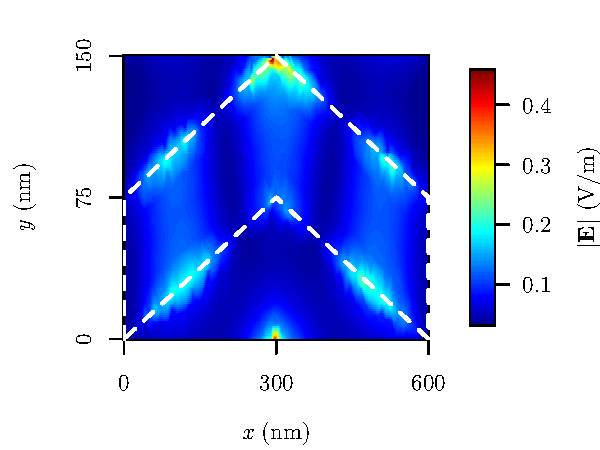
\includegraphics[width=0.49\linewidth]{band-gap-figures/2kg-kg-mode1-zEq41nm.pdf}\label{fig:zzbandgapfields2A}}
	\subfigure[]{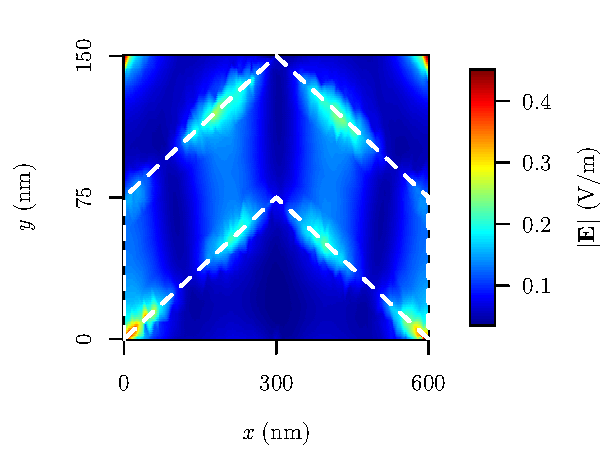
\includegraphics[width=0.49\linewidth]{band-gap-figures/2kg-kg-mode2-zEq41nm.pdf}\label{fig:zzbandgapfields2B}}
	\end{center}	
\caption[The magnitude of electric field, $|\mathbf{E}|$ for the degenerate SPP standing waves at the first BZ. ($xy$ plane)]{The magnitude of electric field, $|\mathbf{E}|$ for the degenerate SPP standing waves at the first BZ. (a) One solution for the $xy$ plane at $z=41\:\nano\metre$ and (b) The second solution for the $xy$ plane at $z=41\:\nano\metre$. \label{fig:zzbandgapfields2}}
\end{figure}

The electric field arrangements for the two possible standing wave modes at the BZ boundary in the grooves (in the $xy$ plane with $z=20 \:\nano\metre$) and in the $xz$ plane (with $y=75\:\nano\metre$), are extracted from the numerical model and plotted in figure \ref{fig:zzbandgapfields}. 
\begin{figure}
	\begin{center}
		\subfigure[]{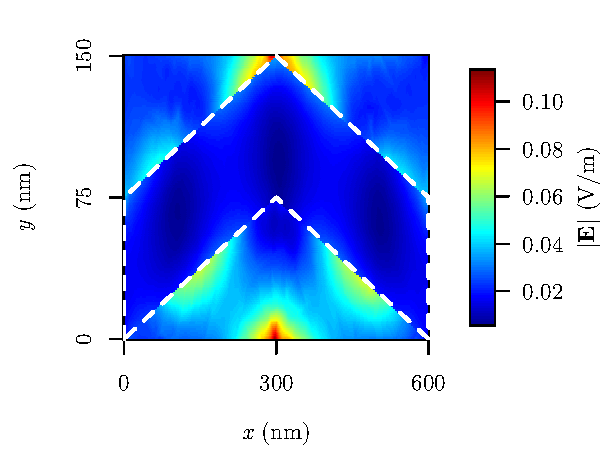
\includegraphics[page=1,width=0.49\linewidth]{band-gap-figures/2kg-kg-mode1.pdf}\label{fig:zzbandgapfieldsA}}
		\subfigure[]{\includegraphics[page=2,width=0.49\linewidth]{band-gap-figures/2kg-kg-mode1.pdf}\label{fig:zzbandgapfieldsB}}\\	
		\subfigure[]{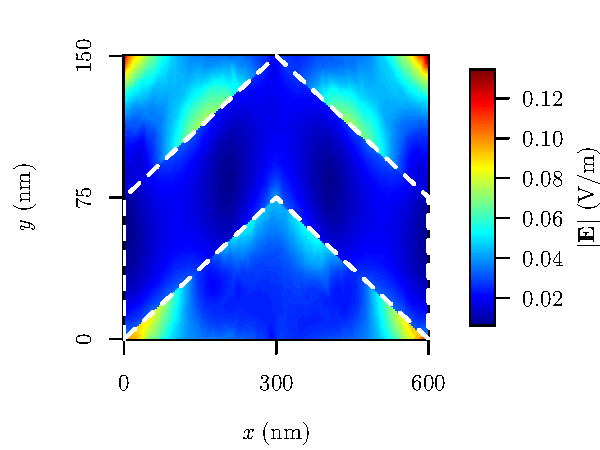
\includegraphics[page=1,width=0.49\linewidth]{band-gap-figures/2kg-kg-mode2.pdf}\label{fig:zzbandgapfieldsC}}
		\subfigure[]{\includegraphics[page=2,width=0.49\linewidth]{band-gap-figures/2kg-kg-mode2.pdf}\label{fig:zzbandgapfieldsD}}		
	\end{center}	
\caption[The magnitude of electric field for the degenerate SPP standing waves at the first BZ. ($xy$ and $xz$ plane)]{The magnitude of electric field for the degenerate SPP standing waves at the first BZ. (a-b) One solution for the (a) $xy$ plane at $z=20\:\nano\metre$ and (b) the $xz$ plane, for $y=75\:\nano\metre$. (c-d) The second solution for the (c) $xy$ plane at $z=20\:\nano\metre$ and (d) the $xz$ plane, for $y=75\:\nano\metre$. \label{fig:zzbandgapfields}}
\end{figure}
These standing waves have three `hotspots' per unit cell, corresponding to a standing wave with the expected period of $\lambda_{SPP}=2\lambda_{gx}/3$. Comparing the magnitude of electric field in the grooves for the $xz$ plane in figures \ref{fig:zzbandgapfieldsB} and \ref{fig:zzbandgapfieldsD}, it is clear that the field arrangements are shifted spatially with respect to each other by $\lambda_{gx}/4$, as one would expect for two standing wave solutions which in general will lie $\pi/2$ degrees out-of-phase with each other. Figures \ref{fig:zzbandgapfieldsA} and \ref{fig:zzbandgapfieldsC} show the calculated field arrangements as figure \ref{fig:zzbandgapcartoon} illustrated. Lying at the same potential, these field arrangements are clearly equivalent, shifted spatially by $\lambda_{gx}$ with respect to each other, yet both occupying a degenerate electromagnetic environment. The magnitude of electric field in the $xz$ plane presented in figures \ref{fig:zzbandgapfieldsB} and \ref{fig:zzbandgapfieldsD} show that the decay of the electric fields into both bounding media are the same for each case, and that neither solution can be labelled more `photon-like' nor `plasmon-like' than the other. This further demonstrates the equivalence in energy of these two standing waves.

The equivalence in energy of these two standing wave solutions can be broken by the removal of the zigzag grating's mirror plane. By making the zigzag asymmetric, the electric field arrangements for both possible standing waves differ in energy and a band-gap may form. This is demonstrated in chapter \ref{c:azigzag}



\section{Anisotropic Propagation of SPP Modes for Self Collimation\label{sec:anisotropic}}

Plasmonic circuits couple and direct SPPs along designed structures to provide a transfer of power and information \cite{Ozbay2006a,Zayats2005}. These optoelectronic devices require the development of SPP optics which behave like their classical optics counterparts.

One of the most crucial roles of these surface-optics is the ability to generate a collimated SPP beam, so that the SPPs may be directed efficiently without any detrimental loss across the device due to divergence. The ideal device should receive incident SPPs over a wide range of angles and the SPPs should then propagate through the component with a narrow angular divergence. This effect has been observed for light in photonic crystals, and was named self-collimation. \cite{Ogawa2005,Kosaka1999}

Recently, such components have been manufactured that use square bi-gratings to manipulate the local curvature of the SPP iso-frequency contour. These gratings have demonstrated self-collimation in the microwave regime \cite{Kim2011} as well as in the visible \cite{Stein2012}. They  have also been designed to achieve all-angle negative refraction of surface waves \cite{Luo2002, Ruan2006}. The work by Stein et al. \cite{Stein2012} showed that the self-collimation effect could be achieved around the M symmetry point in $k$-space due to the mini-gaps formed by band-gapping SPPs over a momentum range of $1\:\micro\metre^{-1}$. It is desirable that this momentum range is large, so as to maximise the angular divergence over which the device could collimate SPPs.

We have found that zigzag gratings possess a mechanism for the collimation of SPPs at a single wavelength. This mechanism is similar to previous work, as it  relies on plasmonic band-gaps to cause anisotropic propagation of SPPs along the surface, which is observed as a deformation of the SPP iso-frequency contours to approximately flat bands with no curvature. However, the azimuthal angle range over which SPPs possess a single direction is far larger than previously reported results, extending over the entire observable region of $k$-space.

Up until now, we have only considered the effects of the $\lambda_{gx}$ periodicity of the zigzag grating with respect to the SPP propagation. With a designed orthogonal pitch of $\lambda_{gy}=150\:\nano\metre$, the diffracted SPPs from a $\mathbf{k}_{gy}$ scattering mechanism have such a large momentum that for the plane of incidence $\phi=0^\circ$, the SPP features will lie well above the visible frequency range. 

However, an important point to note about SPPs travelling along the $\mathbf{k}_{gy}$ direction is that they will be travelling over surface relief grooves and not, like the $\pm\mathbf{k}_{gx}$ surface plasmons, along the zigzag contours. This means that the charge arrangements for standing-waves at the BZ boundaries will differ in energy considerably, as for traditional surface-relief gratings. Plasmonic band-gaps in the $\mathbf{k}_{gy}$ direction are expected, and will be similar to those on typical bigratings. Evidence for these band-gaps are seen in figure \ref{fig:anisotropic-dispersion-diagrams}. The experimental results show the dispersion mapped using the reflectivity of the zigzag grating to indicate the SPP mode positions for a wavelength range of $450<\lambda_0<800\:\nano\metre$ and an angular range $7^\circ<\theta<65^\circ$, for two planes of incidence. One plane of incidence includes the $\mathbf{k}_{gx}$ grating vector ($\phi=0^\circ$) and the orthogonal plane of incidence ($\phi=90^\circ$) contains the $\mathbf{k}_{gy}$ vector. In both cases the $\pm 1\mathbf{k}_{gx}$ scattered SPP is observed. For $\phi=0^\circ$ the SPP dispersion is an asymptotic curve, while for $\phi=90^\circ$ it is seen as a hyperbolic conic intersection, but both map the same SPP in momentum space. For the coupling of light to the SPP in figure \ref{fig:anisotropic-dispersion-diagrams}, the polarisation of the incident light has been rotated $90^\circ$, and so is TM polarised.

\begin{figure}
	\begin{center}
		\subfigure[][$R_{ss}$ at $\phi=0^\circ$]{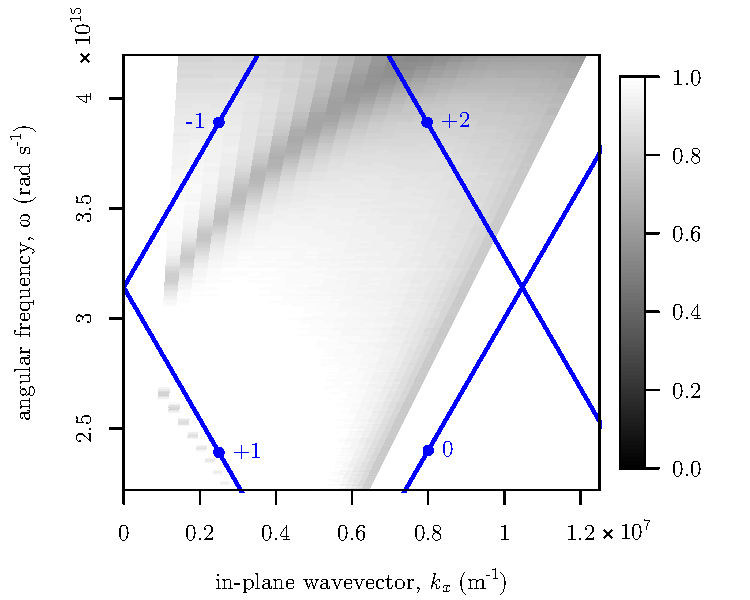
\includegraphics[width=0.45\linewidth]{figure-symzz-AIR-dispersion-rss.pdf}}
		\subfigure[][$R_{pp}$ at $\phi=90^\circ$]{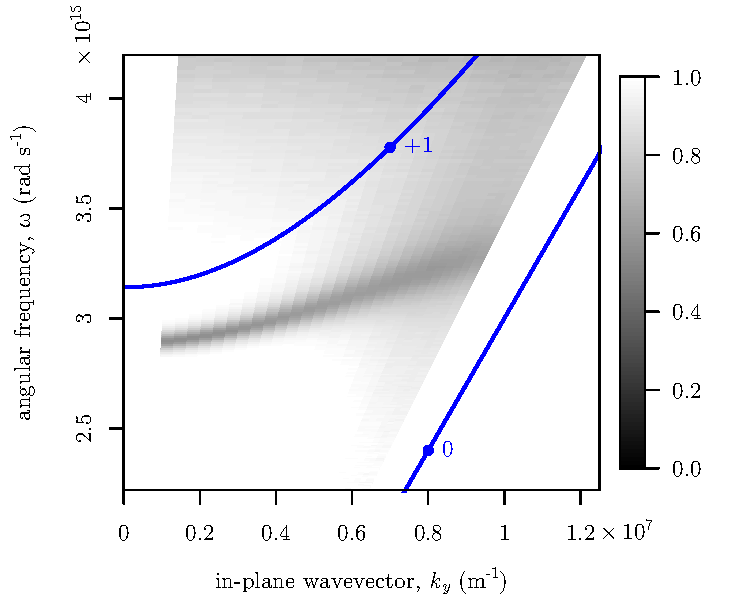
\includegraphics[width=0.45\linewidth]{figure-symzz-AIR-dispersion-rpp-90azi.pdf}}
		\caption{Experimentally obtained dispersion plots for a zigzag grating at $\phi=0^\circ$ and $\phi=90^\circ$\label{fig:anisotropic-dispersion-diagrams}}
	\end{center}
\end{figure}

It is found that in the $\phi=90^\circ$ orientation, the SPP dispersion curve asymptotes far faster than the $\phi=0^\circ$ case. This lower asymptote is evidence of a large band-gap at the first BZ in the $\mathbf{k}_{gy}$ direction, with the mode meeting the BZ boundary with zero group velocity at $2.1\times 10^{7} \metre^{-1}$. This band-gap is the result of the interaction between the $\pm\mathbf{k}_{gx}$ and $\pm\mathbf{k}_{gx}+\mathbf{k}_{gy}$ scattered SPPs which are separated by a single scattering vector that is also a harmonic of the grating surface profile, $\mathbf{k}_{gy}$. Strong interaction is then expected, and the freedom of the charge to organise into energetically dissimilar arrangement in the grooves leads to a large plasmonic band-gap in this direction.

The relevance of this large band-gap to the collimation of SPPs becomes apparent in the evolution in wavelength of the SPP iso-frequency contours mapped using imaging spectrometry, shown in figure \ref{fig:anistropic-zigzag-scattergrams}.

\begin{sidewaysfigure}
	\subfigure[][650 nm]{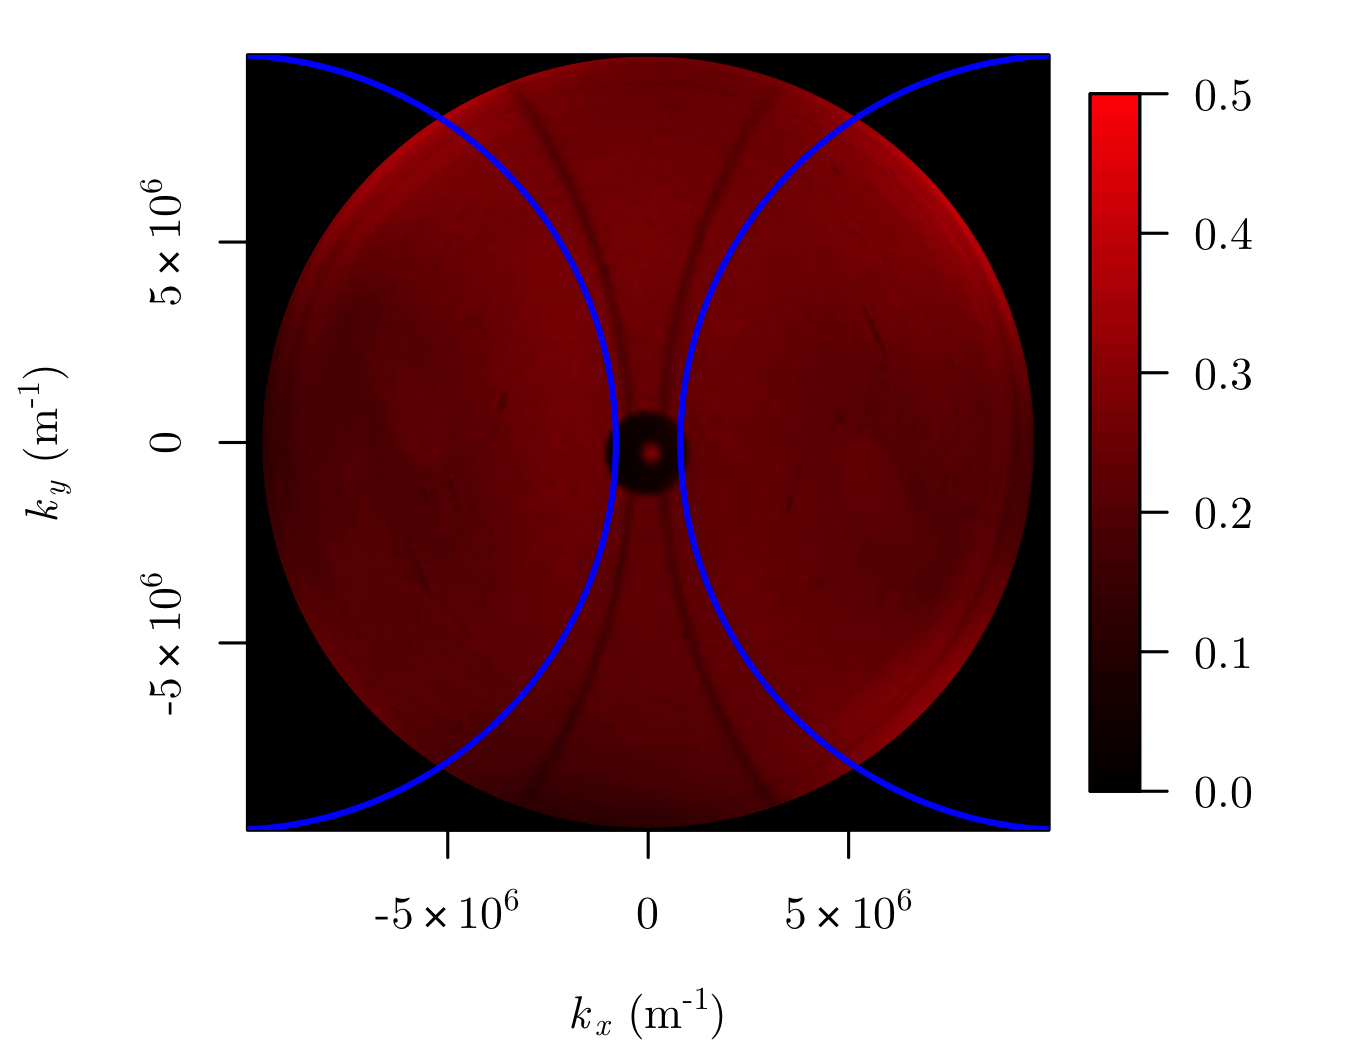
\includegraphics[page=1,width=0.33\textheight]{scattergrams/figure-650nm-scattergram-withaxes.png}}
	\subfigure[][600 nm]{\includegraphics[page=2,width=0.33\textheight]{scattergrams/figure-600nm-scattergram-withaxes.png}}
	\subfigure[][580 nm]{\includegraphics[page=3,width=0.33\textheight]{scattergrams/figure-580nm-scattergram-withaxes.png}}\\
	\subfigure[][550 nm]{\includegraphics[page=4,width=0.33\textheight]{scattergrams/figure-550nm-scattergram-withaxes.png}}
	\subfigure[][500 nm]{\includegraphics[page=5,width=0.33\textheight]{scattergrams/figure-500nm-scattergram-withaxes.png}}
	\subfigure[][450 nm]{\includegraphics[page=6,width=0.33\textheight ]{scattergrams/figure-450nm-scattergram-withaxes.png}}
	\caption[Measured iso-frequency contours of a zigzag grating for a range of wavelengths. ]{Measured iso-frequency contours of a zigzag grating for a range of wavelengths. The blue circles indicate calculated diffraction edges.\label{fig:anistropic-zigzag-scattergrams}}
\end{sidewaysfigure}

The scattergrams map the iso-frequency contours of the $\pm 1\mathbf{k}_{gx}$ scattered SPPs in $k$-space, with the minimum of reflection indicating the SPP mode position as the reflection is suppressed by SPP excitation. The polarisation is set so that the electric field lies orthogonal to the $\mathbf{k}_{gx}$ vector at $k_y=0$, satisfying the TE excitation condition for these SPPs in this plane. As detailed in section \ref{sec:TEexciatation}, the $\pm 2\mathbf{k}_{gx}$ scattered SPPs are not excited with this polarisation, and are not observed. The grating used for these scattergrams is a silver zigzag grating in air as detailed in section \ref{sec:TEexciatation}, with a depth of $d\approx 40 \:\nano\metre$. 

As the frequency increases (the wavelength shifting from red to blue), the $\pm 1\mathbf{k}_{gx}$ scattered SPP contours grow increasingly flat-banded. This is due to the increasing overlap and interaction with the $\pm 1\mathbf{k}_{gx}\pm 1\mathbf{k}_{gy}$ scattered SPPs and the formation of a large band-gap well outside the available momentum space to the free-space light. At $\lambda_0=450\:\nano\metre$, the SPP bands become flat, with essentially no curvature. This scattergram is repeated in figure \ref{fig:450scatter}, with some additional important annotations.

\begin{figure}
\begin{center}
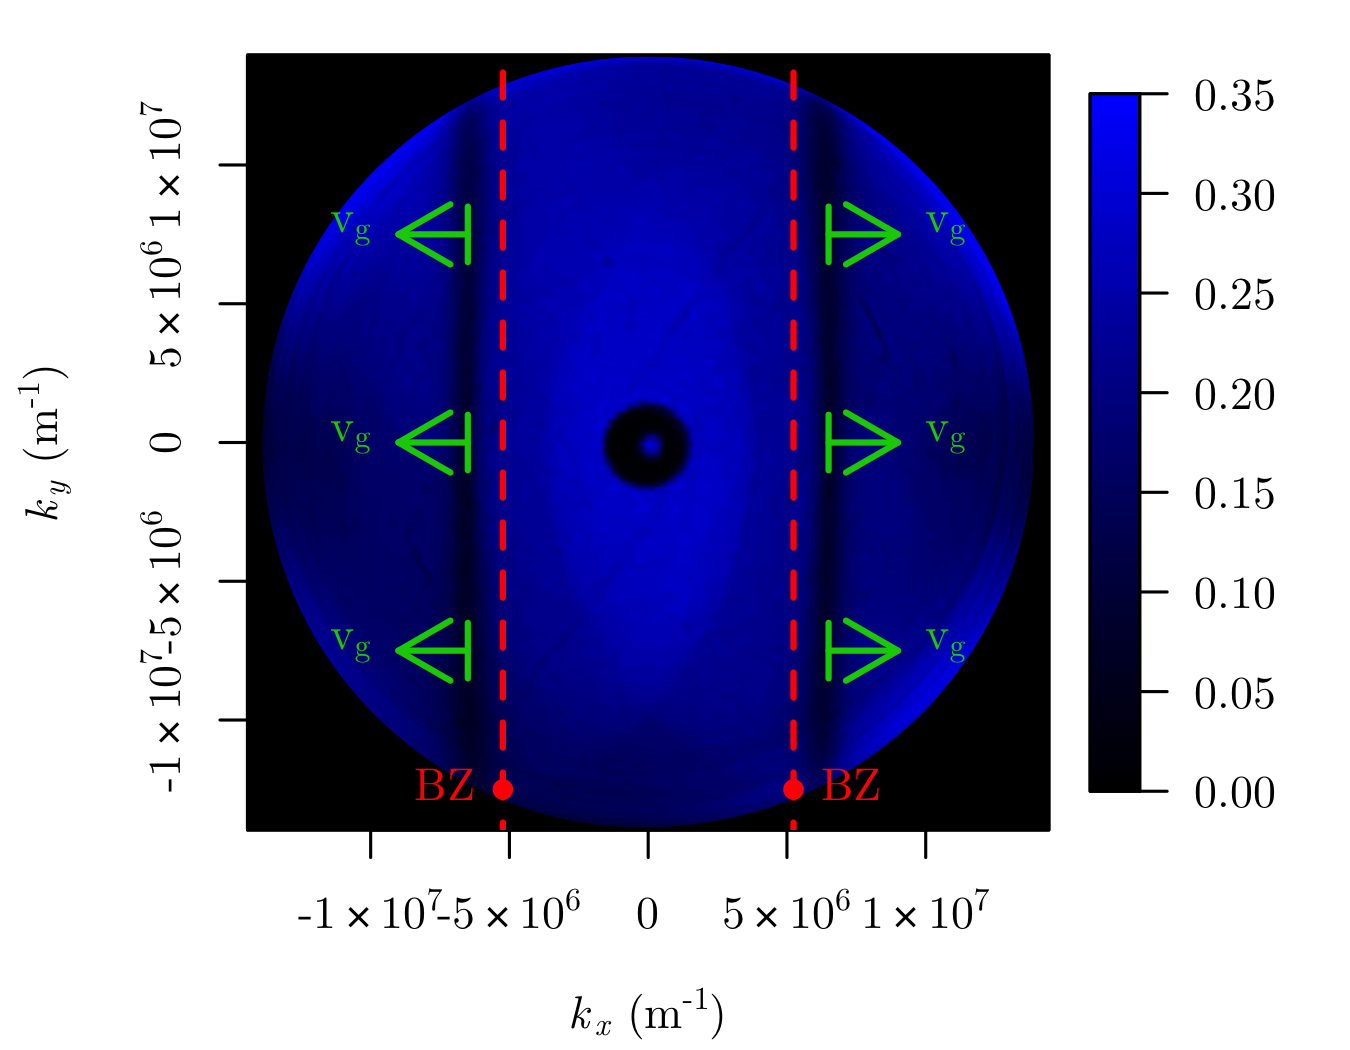
\includegraphics[width=0.6\linewidth]{scattergrams/figure-450nm-collimatedSPPs.png}
\end{center}
\caption[The SPP iso-frequency contours mapped using imaging scatterometery at $\lambda_0=450\:\nano\metre$.]{The SPP iso-frequency contours mapped using imaging scatterometery at $\lambda_0=450\:\nano\metre$. The green arrows show the direction of the SPP group velocity along the contour, indicating that for this wavelength the SPP waves only travel in the $\pm\mathbf{k}_{gx}$ direction. The red dotted lines show the position of the BZ boundary.\label{fig:450scatter}}
\end{figure}

Since the group velocity of the SPP wave is determined from $\mathbf{v}_g=\mathbf{\nabla}\omega(\mathbf{k})$, the direction of the SPP energy flow is in the direction orthogonal to the SPP contour (see chapter \ref{c:oblique} for more details on this inference).  Six example group velocity directions are shown as green arrows in figure \ref{fig:450scatter}, showing that, for a given scattered SPP, the group velocity is only in the $k_x$ direction. This corresponds to a self-collimated SPP wave across a momentum range of at least $2.2\times10^{7} \metre^{-1}$, an order of magnitude higher than previous results \cite{Stein2012}, and successfully collimates SPPs for an incident azimuthal range of $-63.4^\circ<\phi<63.4^\circ$ at $\lambda_0=450\:\nano\metre$. 

An Important observation is to be made of figure \ref{fig:450scatter}; that the $\pm 1\mathbf{k}_{gx}$ scattered SPP contours lie outside of the BZ boundary (red dotted lines). Two comments must be made about this: the first is that the BZ represents the smallest unit cell which, when repeated by translational symmetry operations, reproduces fully the band structure of the system. Clearly, the BZ lying between the two red lines does not replicate the band structure of the grating once translated. This is because the $\pm 2\mathbf{k}_{gx}$ scattered SPPs are not coupled strongly to light in our experiment. The eignestates for the SPPs are still present in the BZ, just not excited by the incident radiation, and so the validity of the BZ holds.
The second point is that the $\pm 1\mathbf{k}_{gx}$ SPPs have passed through the BZ boundary unperturbed. This is important, as if the contours were perturbed at this boundary, the efficiency of the collimation of SPP waves would be impacted. Because band-gaps at the first BZ are forbidden (not just weak) in the $k_x$ direction, unwanted perturbation of the SPP contour at this boundary will not occur. This is a condition due to the mirror symmetry of the zigzag grating surface, and an analogy cannot be found in traditional gratings.


\section{Conclusions}
This chapter has introduced a new type of diffraction grating, a zigzag grating. This grating uses sub-wavelength surface structure to provide a diffractive periodicity to wavelength-scale light. SPPs may be diffractively coupled to using a metallic zigzag grating, and their excitation and band structure are found to depend on the symmetry of the zigzag pattern.

The polarisation of light coupling to SPPs on such a grating is found to be dependent on the diffracted order used. For odd-ordered diffraction, TE polarised light couples to the SPPs, while for even-ordered diffraction, TM polarised light is required. This has been explained using a simple analytical formula which considers the available normal component of electric field to the surface of the grating, and the polarisation selectivity has been demonstrated experimentally on fabricated silver zigzag gratings.

This polarisation selectivity may be found to be of use for plasmonic devices in which polarisation separation is desirable. As an example, the incorporation of zigzag gratings in metal-insulator-metal structures designed for the generation of light could yield a polarisation dispersing light source. These SPP mediated light sources, when incorporated with a zigzag grating, would emit different polarisations of light in to different diffracted orders. Breaking the mirror symmetry of the zigzag pattern provides a route to polarisation-independent absorption of light into SPPs, a topic which is explored in greater detail in chapter \ref{c:azigzag}.

The band structure of SPPs on zigzag gratings is found to be highly dependent on the surface symmetry. Most strikingly, the formation of a band-gap at the first BZ boundary is forbidden by the degeneracy of the allowed standing wave states. 

Using scatterometry, the propagation of SPPs on such surface is shown to be highly anisotropic, due to the large band-gaps which occur orthogonal to the diffraction plane. These highly perturbed SPP contours, combined with the forbidden band-gaps at the first BZ  boundary in the $x$-direction, lead to wide-angle surface wave collimation. The use of zigzag gratings to generate surface-waves with highly directional planar wave-fronts in plasmonic circuits, over a wide range of azimuthal angles, could be of great interest to optoelectronic engineers. Further investigation of this phenomenon is left for future work, with the recommendation of using near-field imaging of SPPs to characterise the surface waves and exploring also the collimating effect of the grating.

